\documentclass[12pt]{report}
\usepackage{rotating}
\usepackage{multirow}
\usepackage{hyperref}
\usepackage{amsfonts}
\usepackage{amssymb}
\usepackage{amstext}
\usepackage{amsmath}
\usepackage{siunitx}
\usepackage{comment}
\usepackage{graphicx}
\usepackage{floatrow}
\usepackage{tikz}
\usepackage{caption}
\usepackage{subcaption}
\usepackage{xcolor} 
\usepackage{longtable} 
\usepackage{tabularx} 
\usepackage{adjustbox} 
\usepackage{diagbox} 
\usepackage{rotating}
% This file contains macros that can be called up from connected TeX files
% It helps to summarise repeated code, e.g. figure insertion (see below).

% insert a centered figure with caption and description
% parameters 1:filename, 2:title, 3:description and label





\newcommand{\figuremacro}[3]{
	\begin{figure}[htbp]
		\centering
		\includegraphics[width=1\textwidth]{#1}
		\caption[#2]{\textbf{#2} - #3}
		\label{#1}
	\end{figure}
}

% insert a centered figure with caption and description AND WIDTH
% parameters 1:filename, 2:title, 3:description and label, 4: textwidth
% textwidth 1 means as text, 0.5 means half the width of the text
\newcommand{\figuremacroW}[5]{
	\begin{figure}[h]
		\centering
		\includegraphics[width=#4\textwidth]{#1}
		\caption[#2]{\textbf{#2} - #3}
		\label{#5}
	\end{figure}
}
%macros for PDFs
\newcommand{\unpolpdf}{$f(x)$}
\newcommand{\longpdf}{$g(x)$}
\newcommand{\transpdf}{$h_{1}^{q}(x)$}

%frgamentations
\newcommand{\IFF}{$H_{1}^{\sphericalangle, q}$}
\newcommand{\CollinsFF}{$H_{1}^{\perp}$}

\newcommand{\Lagr}{\mathcal{L}}
\newcommand{\vy}{\mathbf{y}}
\newcommand{\vx}{\mathbf{x}}
\newcommand{\vxx}{\mathbf{V_{xx}}}
\newcommand{\vyy}{\mathbf{V_{yy}}}
\newcommand{\lag}{\mathcal{L}}
\newcommand{\ma}{\mathbf{A}}
\newcommand{\ptpair}{$p_T^{\pi^+\pi^-} $}
\newcommand{\mpair}{$M_{inv}^{\pi^+\pi^-} $}
\newcommand{\etapair}{$\eta^{\pi^+\pi^-} $}
\newcommand{\dipion}{$\pi^+\pi^-$ }



% inserts a figure with wrapped around text; only suitable for NARROW figs
% o is for outside on a double paged document; others: l, r, i(inside)
% text and figure will each be half of the document width
% note: long captions often crash with adjacent content; take care
% in general: above 2 macro produce more reliable layout
\newcommand{\figuremacroN}[3]{
	\begin{wrapfigure}{o}{0.5\textwidth}
		\centering
		\includegraphics[width=0.48\textwidth]{#1}
		\caption[#2]{{\small\textbf{#2} - #3}}
		\label{#1}
	\end{wrapfigure}
}

% predefined commands by Harish
\newcommand{\PdfPsText}[2]{
  \ifpdf
     #1
  \else
     #2
  \fi
}

\newcommand{\IncludeGraphicsH}[3]{
  \PdfPsText{\includegraphics[height=#2]{#1}}{\includegraphics[bb = #3, height=#2]{#1}}
}

\newcommand{\IncludeGraphicsW}[3]{
  \PdfPsText{\includegraphics[width=#2]{#1}}{\includegraphics[bb = #3, width=#2]{#1}}
}

\newcommand{\InsertFig}[3]{
  \begin{figure}[!htbp]
    \begin{center}
      \leavevmode
      #1
      \caption{#2}
      \label{#3}
    \end{center}
  \end{figure}
}

\newcommand{\drawgraphics}[4]{
    \begin{figure}
		\centering
		\includegraphics[width=#1\textwidth]{#2}
		\caption{#3}
		\label{#4}
    \end{figure}
}

\newcommand{\InsertTable}[4]{
    \begin{table}[htb]
        \centering
        \begin{tabular}{#1}
             #2
        \end{tabular}
        \caption{#3}
        \label{#4}
    \end{table}
}

\newcommand{\pip}{$\pi^+\pi^-$}
\newcommand{\aut}{$A^{sin(\phi_{RS})}_{UT}$}
\newcommand{\etap}{$\eta^{\pi^+\pi^-}$}
\newcommand{\minv}{$M^{\pi^+\pi^-}_{inv}$}
\newcommand{\ptp}{$p^{\pi^+\pi^-}_{T}$}


%%% Local Variables: 
%%% mode: latex
%%% TeX-master: "~/Documents/LaTeX/CUEDThesisPSnPDF/thesis"
%%% End: 

\input{TemplePhD_Packages}


% Change the header; default: Bibliography
\addto{\captionsenglish}{\renewcommand{\bibname}{BIBLIOGRAPHY}}

\captionsetup{belowskip=12pt,aboveskip=4pt}

% Turn off those nasty overfull and underfull hboxes
\hbadness=10000
\hfuzz=50pt

\begin{document}

% Center the chapter titles
\renewcommand{\chaptername}{CHAPTER}
\titleformat{\chapter}[display]{\normalfont\huge\bfseries\centering}{\chaptername\ \thechapter}{20pt}{\Huge}

\newcommand{\mychapter}[2]{
    \setcounter{chapter}{#1}
    \setcounter{section}{0}
    \chapter*{#2}
    \addcontentsline{toc}{chapter}{#2}
}

% Set font parameters
\fontsize{12}{15}
\selectfont

%: ----------------------------------------------------------------------
%: Title page
%: ----------------------------------------------------------------------

\renewcommand\baselinestretch{1.2}
\baselineskip=18pt plus1pt

\setcounter{page}{1}
\begin{titlepage}

\begin{centering} 
{\bf {\Large  MEASUREMENTS OF TRANSVERSE SPIN DEPENDENT $\pi^+\pi^-$ AZIMUTHAL CORRELATION ASYMMETRY AND UNPOLARIZED $\pi^+\pi^-$ CROSS SECTION IN $pp$ COLLISIONS AT $\sqrt s  = 200$ GeV AT STAR}}

\vspace{1cm}
\noindent\makebox[\linewidth]{\rule{16cm}{0.4pt}} \\ 
\vspace{1cm}
A Dissertation                       \\
Submitted to                         \\
the Temple University Graduate Board \\
\vspace{1cm}
\noindent\makebox[\linewidth]{\rule{16cm}{0.4pt}} \\ 
\vspace{1cm} 
In Partial Fulfillment               \\
of the Requirements for the Degree   \\
DOCTOR OF PHILOSOPHY                 \\
\vspace{1cm} 
\noindent\makebox[\linewidth]{\rule{16cm}{0.4pt}} \\ 
\vspace{1cm} 
by                                   \\
Babu R.\ Pokhrel                       \\
\today \\
\end{centering}                      

\vspace{1cm}
\noindent{Examining Committee Members:}\\
\vspace{0.20cm}

\noindent {Bernd Surrow, Department of Physics, Advisory Chair}        \\
{Andreas Metz, Department of Physics}                                        \\
{Jim Napolitano, Department of Physics}                                       \\
{Anslem Vossen, External Reader}

\end{titlepage}

\pagenumbering{roman}

%: ----------------------------------------------------------------------
%: Front matter: dedication and acknowledgments
%: ----------------------------------------------------------------------
\renewcommand\abstractname{\normalfont\huge\bfseries\centering ABSTRACT}
\begin{abstract} 
\thispagestyle{plain}
\addcontentsline{toc}{chapter}{ABSTRACT}
\doublespacing
The transversity distribution function, $h_1^{q}(x)$, where $x$ is the longitudinal momentum fraction of the proton carried by quark $q$, encodes the proton's transverse spin structure at the leading twist. Extraction of it is difficult because of its chiral-odd nature. However, it can be coupled with a spin-dependent interference fragmentation function (FF), $H_1^{\sphericalangle, q}$, in polarized proton-proton ($p^\uparrow p$) collisions. The coupling of $h_1^{q}(x)$ and $H_1^{\sphericalangle, q}$ produces an experimentally measurable azimuthal correlation asymmetry, $A_{UT}$, between the spin of the fragmenting quark and the final state dihadron. A model-independent extraction of transversity from these measurements relies on the knowledge of dihadron FFs, namely the unpolarized dihadron FFs, $D_1^{h_1h_2/q(g)}$ for quarks, \emph{q} (gluons, \emph{g}). Extraction of these FFs requires measurements of the unpolarized dihadron cross section in $pp$ collisions, which are desperately needed. In $pp$ collisions, the unpolarized cross-section measurement provides access to the $D_1^{h_1h_2}$ for both quarks and gluons. This thesis outlines the measurements of the \dipion azimuthal correlation asymmetry in the mid-pseudorapidity ($|\eta|<1$) region using the RHIC run 2015 polarized $pp$ data and the measurement of the unpolarized \dipion cross-section measurement in the invariant mass bins in the forward and backward pseudorapidity regions with respect to the polarized beam using the RHIC run 2012 $pp$ data at $\sqrt{s}=200$ GeV.   
\end{abstract}


\setcounter{page}{2}
\addcontentsline{toc}{chapter}{ACKNOWLEDGEMENTS}
\chapter*{ACKNOWLEDGEMENTS}

Writing this thesis was a challenging endeavor, and I owe its completion to the unwavering support and influence of numerous individuals who have impacted my Ph.D. journey and beyond. I extend my heartfelt gratitude to those who played pivotal roles in my academic success.

First and foremost, I sincerely thank my advisor, Dr. Bernd Surrow, whose continuous guidance and support have been instrumental throughout this journey. I am also deeply grateful to my thesis committee members, Dr. Andreas Metz and Dr. Jim Napolitano, for their invaluable feedback and contributions to my academic growth. The Classical Mechanics and Particle Physics courses with Dr. Metz during my first and fourth semesters and the initial two semesters of Quantum Mechanics with Dr. Napolitano significantly enriched my knowledge and understanding.

I want to thank Dr. Marco Radici, Dr. Metz, and Dr. Christopher Cocuzza for their unwavering support. They have provided theoretical predictions and actively participated in discussions, offering valuable theoretical perspectives that complement the measured experimental results. 

I appreciate the entire Physics department and administration's administrative assistance during this challenging period.

My gratitude also extends to the NUPAX particle physics research group led by Dr. Surrow. Being a part of this group has been an enriching experience, thanks to the dedicated particle physics enthusiasts and experts who provided continuous support and guidance. I am indebted to Dr. Matt Posik, Dr. Jae Nam, Dr. Amilkar Quintaro, Dr. Nicholas Lukow, and Navagyan Ghimire for their motivation and encouragement.

My parents have been my ultimate academic role models, as they never compromised on providing quality education despite financial hardships. Their profound understanding of the value of education, shaped by their personal experiences, has been a driving force in my pursuit of knowledge. I consider myself truly fortunate and blessed to have such incredible parents.

I am deeply grateful to my wife, whose constant support and motivation have been my pillars of strength throughout this journey. Her love and care have made my life more comfortable, and I cannot imagine going through this endeavor without her unwavering presence.

Lastly, I express my heartfelt thanks to all my friends, Navagyan Ghimire, Jay Poudel, Dr. Santosh Neupane, Anoj Aryal, and Biru K.C., who have stood by me and supported me in every step of this journey. Their companionship has made this challenging path more bearable and enjoyable.









%: ----------------------------------------------------------------------
%: Contents
%: ----------------------------------------------------------------------

\setcounter{secnumdepth}{5}
\setcounter{tocdepth}{5}
\renewcommand{\contentsname}{TABLE OF CONTENTS}
\tableofcontents

%: ----------------------------------------------------------------------
%: List of figures and tables
%: ----------------------------------------------------------------------
\begingroup
\renewcommand\addvspace[1]{}
\setlength\parskip{\baselineskip}
\renewcommand{\listfigurename}{LIST OF FIGURES}
\renewcommand{\listtablename}{LIST OF TABLES}

\listoffigures
\addcontentsline{toc}{chapter}{LIST OF FIGURES}

\listoftables
\addcontentsline{toc}{chapter}{LIST OF TABLES}

\endgroup

%: ----------------------------------------------------------------------
%: Glossary: Not used in this version of the template
%: ----------------------------------------------------------------------

% Tie in external source file for definitions: /TOC/glossary.tex
% Glossary entries can also be defined in the main text. See glossary.tex
% \include{TOC/glossary}

% \begin{multicols}{2}      % \begin{multicols}{#columns}[header text][space]
% \begin{footnotesize}      % scriptsize(7) < footnotesize(8) < small (9) < normal (10)
%
% \printnomenclature[1.5cm] % [] = distance between entry and description
% \label{nom}               % target name for links to glossary
%
% \end{footnotesize}
% \end{multicols}

%: ----------------------------------------------------------------------
%: Main document section
%: ----------------------------------------------------------------------

\addtocontents{toc}{\vspace*{0.25in}}
%\addtocontents{toc}{\contentsline{chapter}{\numberline{CHAPTER}}}
%\addtocontents{toc}{\contentsline{chapter}{\numberline{CHAPTER}}}
%\addtocontents{toc}{\protect\contentsline{CHAPTER}{\protect\numberline{CHAPTER}}}
\newpage
\pagenumbering{arabic}
\setcounter{page}{1}

\chapter{INTRODUCTION}
\DeclareGraphicsExtensions{.png,.jpeg,.pdf} 

 \section{Overview}
 Humans have always been curious about the composition of the matter around them. However, the reality is that all entities in the universe are built upon the same foundation - electrons, protons, and neutrons. The protons and neutrons are commonly called nucleons. This leads us to wonder why objects display various properties. Thankfully, a lot of these queries have already been resolved. By comprehending the traits and configurations of these fundamental components, we can understand the formation of atoms, molecules from atoms, and how molecules combine to create matter in our surroundings.

 To understand the properties of matter around us, it's essential to comprehend the nature of its building blocks. One pertinent question is whether these ``building blocks'' are breakable or contain substructures. Unfortunately, these particles are incredibly small, making it difficult to examine them for their properties. The only way to gain insight into their composition is by colliding them with high energy and observing the resulting debris. These experiments, which involve the collision of leptons (spin-1/2 fermions), nucleons (composite structures containing quarks), and heavy ions have provided crucial early information. Many sophisticated experiments are underway, answering several unanswered questions while uncovering new mysteries. 

We currently understand that electrons are fundamental particles. On the other hand, protons and neutrons comprise smaller components called quarks and gluons which bind them together. Quarks are fermions with fractional electromagnetic charge, while gluons are neutral charge (electromagnetic) spin-1 intermediate bosons that act as force carriers between quarks within nucleons by the strong force. Hadrons, which consist of three quarks, are classified as mesons or baryons based on their quark content\footnote{mesons contain a quark and anti-quark pair and baryons contain three quarks.}. The unique properties of nucleons arise from the interactions between quarks and gluons, commonly called partons. Therefore, uncovering the parton structure of nucleons is a critical area of study in high-energy physics. 

There has been a development of theory that successfully explains the bound structure of nucleons. A theory that explains electromagnetic interaction between electromagnetically charged particles via virtual photon exchange is called quantum electrodynamics (QED). The QED, combined with the theory of weak decay of particles via the intermediate vector bosons ($z,\ W^\pm $) by Winberg and Salam, is now commonly called an electroweak theory. The theory of strong interaction, called quantum chromodynamics (QCD), describes the strong interaction between quarks via the exchange of color-charged-gluon.   

After the discovery of the EMC collaboration in 1989, suggesting that the valence quarks contribute little to none to the nucleon's spin, the spin structure of the nucleon remains an unsolved problem thus far, which is widely known as ``proton spin puzzle". 
The unpolarized nucleon structure is known to much higher precision; however, the polarized structure is still not fully understood, specifically the contribution of gluon polarization. It is important to understand how the quarks and gluons dynamics and their spin contribute to the total nucleon property given by the parton distribution functions (PDFs). At the leading twist, three PDFs are enough to describe the nucleon structure: unpolarized (or helicity averaged), helicity PDF, and transversity PDF. Spin asymmetry measurements in polarized  semi-inclusive deep inelastic scattering  (SIDIS) and polarized proton-proton collision ($pp$) have served as crucial tools to understand the (polarized) nucleon structure. The transversity PDF, which is less understood than other PDFs, is lately gaining more attention for its correlation with the tensor charge. This thesis specifically outlines the measurement of two crucial observables, azimuthal correlation asymmetry and the unpolarized cross section, via \dipion channel necessary for the precision measurement of transversity PDF.    

This thesis outline is as follows. In this chapter, I will first provide an overview of elementary particles and a model that describes them. I will also provide the basics of the QCD theory and relevant terminology that will be used frequently hereafter. In the second chapter, I will be more specific about the proton's structure, providing current experimental and theoretical progress, specifically on the transverse momentum-dependent structure of the proton. Chapter 3 will provide experimental aspects; the relativistic heavy ion collider (RHIC) and the solenoidal tracker at RHIC (STAR). Chapters 4  and 5 provide measurement details and results for the  azimuthal correlation asymmetry and unpolarized \dipion cross section. Finally, in Chapter 6, I will summarize the thesis with the relevant outcomes of the measurements. More details, which are not appropriate in the main body of this thesis, will be provided in the appendices. I will refer to the respective appendix whenever relevant in the main body. 

\section{Review of Elementary Particles}

The elementary particle is defined as the fundamental building block of matter, yet this designation is subject to revision as experimental techniques and theoretical frameworks evolve. Whether a particle is elementary or composite is contingent upon the sensitivity of experimental methods and the extent of scientific understanding at a given time. Thus, the characterization of particles as elementary may not be absolute but reflects our current knowledge and technological capability.
 
Initially, the electron, proton, and neutron were considered the fundamental particles, unbreakable without substructures, until the discovery confirmed that the proton is not fundamental: it has something more fundamental structure. As Rutherford's scattering experiment led to the discovery of the atomic nucleus and, eventually, protons and neutrons, the deep inelastic scattering experiment (DIS) led to the discovery of the internal structure of the proton, the quark, as shown in Figure \ref{fig:protonstr}. 
\begin{figure}
    \centering
    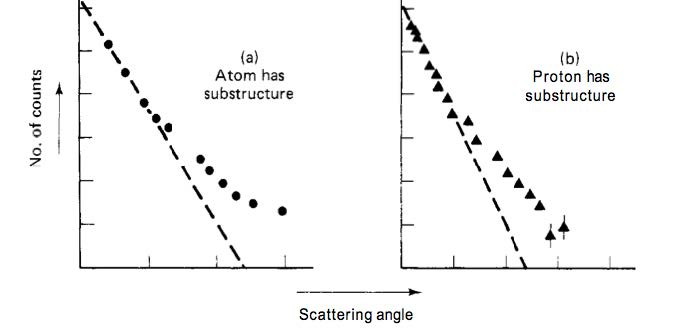
\includegraphics[scale=1.2]{MisImages/martin_halzen_quark.jpg}
    \caption{Left: In Rutherford scattering, the number of particles deflected through large angles indicates that the atom has an internal structure. Right: In deep inelastic scattering, the number of particles scattered through large angles indicates that the proton has an internal structure (quarks). The dashed line represents the expected distribution if the positive charge is uniformly distributed in an atom (left) and proton (right) \cite{HalzenMartin1984}.}
    \label{fig:protonstr}
\end{figure}

Studying the inner workings of a nucleon and its quarks is a complex process that requires advanced detector technologies and particle colliders. These tools allow us to collide particles with enough energy to reveal their inner structure. The wavelength of the probe used in a particle collider is crucial, as it must be smaller than the de-Broglie wavelength\footnote{$\lambda = h/p$, where $h$ = Planck's constant, $p$ = momentum} to probe the nucleon effectively. 

It's worth noting the discovery of elementary particles. Heavier mass particles are produced as the energy of smashing particles increases. Lighter mass particles were discovered first, followed by heavier ones, due to the advancement of particle colliders that achieved higher energy limits.
       
The development of particle discovery started in the 19th century when the modern atomic theory was established. At that time, the exploitable size is $\sim 10^{-10}$m, which is the size of an atom. In 1897, J. J. Thomson discovered an electron and its charge-to-mass ratio by studying the deflection of cathode rays in the external magnetic field \cite{electronJJ}. However, the charge neutrality and large mass of an atom beg speculation that there must be something more massive than an electron and positive in charge that compensates for the electron's charge. This was later confirmed by Rutherford's $\alpha-$scattering experiment \cite{GigerMarsden}, where he passed an $\alpha-$particles\footnote{Helium nucleus consisting of two protons and two neutrons with +2 net charge.} on a gold foil and observed the spectrum of the scattered particles. He observed large deflection in a few of the $\alpha -$particles; however, most remained undisturbed, suggesting that a hard and positive object is in charge at the center and a vast space all around. Rutherford coined the name ``proton" for the nucleus of a hydrogen atom. In 1914, Neils Bhor proposed a model of a hydrogen atom as a negatively charged electron encircling around a positively charged proton at its center. 

There was a problem with Bohr's model, as it failed to explain the atomic structure of higher atomic number elements, for example, a helium atom with two electrons and two protons but four times as massive as hydrogen. It took about two decades until Chadwick discovered the neutron$-$a electrically neutral particle with a mass similar to that of the proton$-$in 1932 \cite{chadwickNeutron}. How positively charged protons reside within the nucleus of size ($\sim 10^{-15}$m) was still puzzling. There should be a stronger force  between nucleons that compensates for the repulsive force and is strong enough to hold protons and neutrons. Yukuwa proposed a theory in 1934 known as the meson theory \cite{Yukawa:1935xg}. He suggested that there should be a force carrier particle, like a photon in electromagnetic interaction, which holds nucleons together, which he called a ``meson". He calculated the mass of the meson to be intermediate between the mass of an electron and a proton. The Yukuwa meson was later discovered as a $\pi-$meson (pion) in 1947. The $\mu-$meson (muon) was also discovered simultaneously with the pion by Powel and co-workers. The muon is the lighter version of an electron and has nothing to do with the strong force.

 Relativistic quantum mechanics started after Dirac's famous relativistic formula,
 \begin{equation}
     E^2 = \vec{p}^2c^2 + m^2 c^4
 \end{equation}
where $E$ is the energy, $\vec{p}$ is the three momentum vector, $m$ is the mass of the particle, and $c$ is the speed of light, the solution of which suggested the existence of antiparticles from the negative energy solution of the relativistic equation, which was not well accepted at that time. However,  the discovery of the positron$-$an positively charged electron$-$ triumphed Dirac's theory in 1931.  Later in 1955 and 1956, antiparticles of proton and neutron, respectively, were discovered.

The discovery of a neutrino follows back to 1930. The missing energy in the nuclear $\beta -$decay kept Pauli skeptical about energy conservation. Fermi proposed that another non-interacting, neutral, and mass-less particle should be emitted along with the electron in the $\beta-$decay. Based on the variation in the energy of the emitted electron considerably, there should not only such particles but two of those are produced. Those particles are named ``neutrinos" by Fermi. 

In late 1947, the neutral kaon ($K^0$) was discovered by Rochester and Butler \cite{Rochester:1947mi} looking at the cloud chamber photograph where it decays to the charge secondaries $\pi^+$ and $\pi^-$. The charged kaon ($K^+$) was discovered in 1949 by Powel. In time, many more particles were found- the $\eta$, the $\phi$, the $\omega$, the $\rho$'s, etc. Heavier particles, $\Lambda$'s, $\Xi$'s, $\Sigma$'s, and $\Delta$'s, were discovered in successive years, which are collectively called strange particles as they produced strangely in the time scale of $\sim 10^{-23}$ seconds and decay relatively slower ($\sim 10^{-10}$ s),  produced by a strong force, and decayed by a weak force. Most of the elementary particles were discovered by the year 1960's making particle physics complete chaos with a swarm of particles. 

To handle this chaos of particles, Murray Gell-Mann proposed a 
``Eightfold Way" of classifying (anti-)particles in 1961 \cite{GellMann:1962}, where he arranged particles in different geometrical patterns (e.g., hexagon to represent meson octet\footnote{eight member family} and a triangular array to represent baryons decuplet\footnote{ten member family}) based on their charge and strangeness. This way of classifying particles led to the discovery of the omega-minus ($\Omega^-$), the missing spot in Gell-Mann's baryon decuplet, and he boldly predicted this particle to exist. The``Eightfold Way" of classifying particles served as a periodic table and initiated the modern era of particle physics.

Later in 1964, the ``Quark Model'' (QM) was proposed by Gell-Mann \cite{GellMann:1964} and independently by Zweig \cite{Zweig:1964}, which suggests that the hadrons\footnote{Baryons and mesons} comprise more fundamental substructures, which Gell-Mann named it ``quarks''. (Anti-)Baryons are composed of three (anti-)quarks, and mesons are composed of a pair of a quark and an antiquark. Quarks come in three flavors; up ($u$), down ($d$), strange ($s$), and three corresponding anti-quarks; anti-up ($\bar{u}$), anti-down($\bar{d}$), and anti-strange ($\bar{s}$). All the quarks have a fractional charge; $u$ has $\frac{2}{3}e$, $d$ and $s$ have $\frac{-1}{3}e$, and their antiparticles have the same magnitude charge, but of opposite sign. Combining these three fundamental quarks, all the baryons and mesons could be reconstructed successfully.  

Besides the intriguing description of the QM, it failed to explain some obvious questions about the fractional charges of (anti-)quarks,  unobserved free (anti-)quarks, and violating the Pauli exclusion principle. Even though the quarks are confined within the hadrons, their existence as a point particle has been observed by the inclusive deep inelastic experiment (DIS), similar to the Rutherford scattering experiment, where most probed particle passes unaffected. In contrast, some are hard-deflected, as shown in figure \ref{fig:protonstr}, which strongly supports the QM. In 1964, O. W. Greenberg suggested the concept of the ``color charge" to the quark to address the QM skepticism. He suggested that each quark, in addition to the fractional electromagnetic charge, has a ``color charge'', which comes in three colors, ``red", ``blue'' and ``green''. A hadron with quarks of different colors (that form a colorless state)is allowed by the exclusion principle. A colorless state is a combination of color and anti-color or a combination of all primary colors in equal proportion. This also explains why quarks are always present within the hadrons and do not exist individually.   

In 1974, the revolutionary $J/\psi$ meson was discovered at Brookhaven National Laboratory (BNL) \cite{E598:1974sol} and Stanford Linear Accelerator (SLAC) \cite{SLAC:1974ind} simultaneously. The $J/\psi$ is a bound state of the charm and anti-charm quarks ($c\bar{c}$)\cite{Clavelli:1974}, which is about three times heavier than the proton and has a much longer lifetime ($10^{20}\ s$). The charm quark was suggested by Borken and Glashow, speculating the parallel between already discovered four types of leptons ($e$,$\mu$, $\nu_{e}$, $\nu_{\mu}$) and only three quarks ($u$, $d$, and $s$). In the successive years, more charmed baryons were discovered (e.g., $\Lambda^+_c (udc)$, $\Sigma_c^+ (uuc)$, $D^0(c\bar{u})$, $D^+(c\bar{d})$), which established the $J/\psi$ as $c\bar{c}$ and again revive the QM. Moreover, the discovery of the ``tau" ($\tau$) in 1975 \cite{Tau:1975} and ``upsilon" ($\Upsilon (b\bar{b})$) in 1977 \cite{Upsilon:1977} adds two leptons (presuming $\nu_{\tau}$) and a ``bottom" or ``beauty" quark. After discovering the ``top'' quark in 1984 \cite{Top:1995}, the quark-lepton symmetry is restored with the six leptons and six quarks. 


\section{Fundamental Forces, Gauge Bosons and The Standard Model}
\subsection{Fundamental Forces and Gauge Bosons}
Four fundamental forces of nature govern the universe's existence: gravity, strong, weak, and electromagnetic forces. All these fundamental forces are discussed in detail in this section. 
\subsubsection{Gravitational Force}
The gravitational force ($F_G$) between two masses varies as an inverse square of their distance ($F_G \sim 1/r^2$). In addition, it is scaled by the masses of objects of interest ($F_G \sim m_1*m_2$). Since this force is more compensated by the concentration of the mass than distance, it's a long-range force. Even though the galaxies are millions of light years apart, they mutually attract each other, maintaining a stable orbit. Albeit gravitational force controls the macroscopic worlds, it is not realizable at the microscopic level. It is negligibly weak at the elementary particle level, which is $\sim 10^{-42}$ times smaller than the electromagnetic force. At the elementary particle level, it becomes significant at the Planck scale ($\sim 10^{-35}$ m), which is extremely small, or at the Planck energy ($\sim 10^{19}$ GeV), which is an extremely high energy, hard to be realizable in real life.       
\subsubsection{Electromagnetic Force}
The nature of electromagnetic force is similar to the gravitational force, except that it is associated with electromagnetically charged particles. It also varies as an inverse square of the distance between the charged particles. It is attractive for the unlike charges and repulsive for the like charges. It is the decisive force that binds electrons and the nucleus to form an atom, atoms together to form molecules, and molecules to form matter that we see in our everyday life. It is also a long-range force, which is $\sim 10^{42}$ times stronger than the gravitational force and a thousand times weaker than the strong force. The charged particles, the electromagnetic field, and their interactions are described by a mathematical framework called Quantum Electrodynamics (QED).   

The gravitational and electromagnetic forces share a common nature: they are long-range forces that vary as an inverse power of distance, $F\sim r^{-n}$. These forces can be felt in everyday life, such as the mutual attraction between the sun and the planets, and the high and low tides on Earth are due to the gravitational. A tiny magnet aligning north-south, the aurora borealis in the polar region, to name a few, are electromagnetic phenomena due to the Earth's magnetic field.  
\subsubsection{Strong Force}
The strong force is about a thousand times stronger than the electromagnetic force, hence the name ``strong force". It is responsible for binding quarks within the nucleon by exchanging a force carrier particle, gluons, and can be felt to a very short distance, a few hadrons in diameter. It behaves as $\sim \exp ^{-r/r_0}/r^2$, where $r_0 \sim 10^{-15}$ m is a hadron diameter and can reach up to $r\leq r_0$. This is the reason why quarks are always confined within the hadrons.   
\subsubsection{Weak Force}
The weak force operates over extremely short distances on the scale of subatomic particles. Its range is governed by the exchange of W and Z bosons, which are the force carriers of the weak force. The range of the weak force is typically on the order of $10^{-18}$ m. The weak force is primarily associated with beta decay, where a neutron can decay into a proton, an electron, and an electron antineutrino. It also involves other particle interactions, including star nuclear fusion reactions.
\subsection{The Standard Model}
The Standard Model (SM) of particle physics is a theoretical framework describing the universe's fundamental particles and forces. It provides a comprehensive understanding of three fundamental forces: the electromagnetic force, the weak nuclear force, and the strong nuclear force. Gravity, the fourth fundamental force, is not included in the Standard Model and is described by a separate theory called general relativity.

SM classifies elementary particles into two categories: quarks and leptons, as shown in figure \ref{fig:sm}. Quarks are the building blocks of protons and neutrons, which make up atomic nuclei. There are six types of quarks: up, down, charm, strange, top, and bottom. Leptons include the electron, muon, and tau particles and their corresponding neutrinos. Each particle has its antiparticle counterpart, with opposite charge and other properties.
\begin{figure}[h]
    \centering
    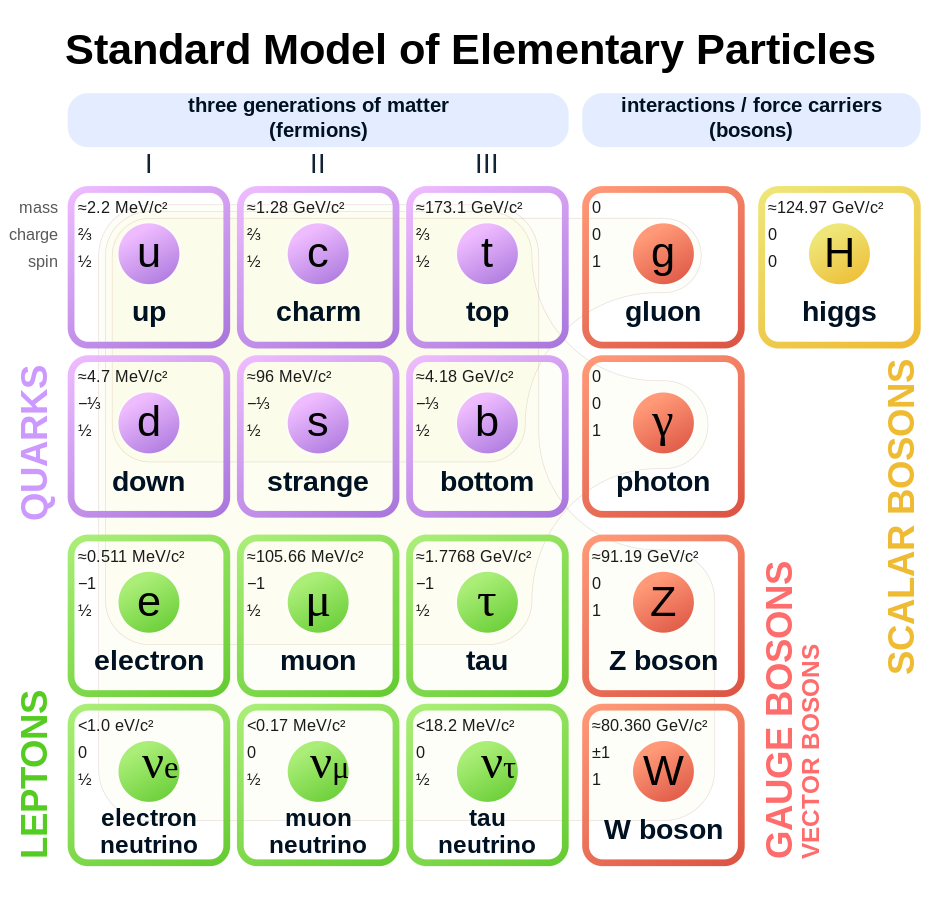
\includegraphics[scale=0.4, trim={0cm 0cm 0cm 2.7cm},clip]{MisImages/Standard_Model_of_Elementary_Particles.svg.png}
    \caption{The standard model of elementary particles \cite{sm}.
    }
    \label{fig:sm}
\end{figure}

The Standard Model describes the fundamental forces as exchanges of particles called gauge bosons. The photon mediates the electromagnetic force, the $W$, and $Z$ bosons mediate the weak nuclear force, and the gluons mediate the strong nuclear force. These gauge bosons carry the forces between particles and govern their interactions.

The Higgs boson is a particle that was discovered in experiments at the Large Hadron Collider (LHC) in 2012 \cite{ATLAShiggs:2012, CMShiggs:2012}. It is associated with the Higgs field, which permeates all of space. The Higgs field gives mass to other particles through their interactions with it. The discovery of the Higgs boson confirmed the mechanism responsible for particle mass in the Standard Model.

\section{Strong Interaction and Quantum Chromodynamics}
Quantum chromodynamics (QCD) is a gauge field theory that describes the strong interactions of colored quarks and gluons in the SU(3) component of the SU(3)$\times$ SU(2)$\times$ SU(1) standard model of particle physics. The QCD lagrangian is given by \cite{Workman:2022}
    \begin{equation}
        \mathcal{L} = \sum_q \bar{\psi}_{q,a}(i\gamma^\mu \partial_\mu \delta_{ab} - g_s \gamma^\mu t^C_{ab} \mathcal{A}^C_\mu - m_q \delta_{ab})\psi_{q,b}-\frac{1}{4}F^A_{\mu\nu}F^{A \mu \nu},
    \end{equation}
where repeated indices are summed over. The $\gamma^\mu$ are Dirac $\gamma-$matrices. The $\psi_{q,a}$ are quark field spinors for a quark flavor $ q$ and mass $m_q$, with color index $a$. The color index $a$ runs from 1 to 3, corresponding to the number of color charges in the QCD ($N_c = 3$). The gluon field is represented by $\mathcal{A}^C$, where $C$ runs from 1 to 8 representing eight types of gluons, which transform under the adjoint representation of the SU(3) color group. The $t_{ab}^C$ are the generators of the SU(3) group in the form of eight 3$\times$3 matrices, which encodes the fact that gluon's interaction with the quark rotates the quark's color in SU(3) space. The $g_s(= \frac{\alpha_s^2}{4\pi})$ is a QCD coupling constant, which is the fundamental parameter of the QCD. The $F_{\mu\nu}^A$ is a field tensor given by 
   \begin{equation}
       F_{\mu\nu}^A = \partial_\mu \mathcal{A}^A_\nu - \partial_\nu \mathcal{A}_\mu^A - g_s f_{ABC}\mathcal{A}_\mu^B\mathcal{A}_\nu^C, 
       \end{equation}
with $[t^A,t^B]= if_{ABC}t^C$, where $f_{ABC}$ are the structure constants of the SU(3) group. 

The QCD theory applies when the strong coupling constant $\alpha_s$ is small, at which quarks are essentially ``free'' within the nucleon. This regime corresponds to the very high energy limit (or a very short distance), where QCD perturbation theory successfully describes the strong interaction between partons. However, the self-gluon  interaction makes the $g_s$ to be varied with the scale of the process, which causes $g_s$ to be small in the short distance (high energy) and large in the longer distance (small distance), leading to the phenomena called ``asymptotic freedom". At the leading order, the strong coupling constant $\alpha_s$ can be expressed as \cite{Surrow:2017}
\begin{equation}
    \alpha_s(Q^2) = \frac{4\pi}{(11-2n_f/3)ln(\frac{Q^2}{\Lambda^2})},
\end{equation}
where $n_f$ is the number of quark flavors and $\Lambda$ is a free scale parameter. The logarithmic dependence of the $\alpha_s$ is because the anti-screening of the effective color charge is because of the gluon bubbles, as shown in figure \ref{fig:glueball}. In any cases when $(11-2n_f/3)>0$, the anti-screening due to the gluon self-interaction dominates, and as a consequence, the $\alpha_s$ decrease with increasing $Q^2$ and becomes relatively weak at the shorter distances. The experimental measurement of $\alpha_s(Q^2)$ as a function of $Q$ from the world data is shown in figure \ref{fig:alphasvsQ}.
\begin{figure}
    \centering
    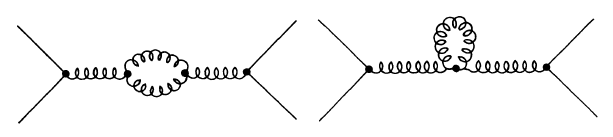
\includegraphics[scale=0.5]{MisImages/glueballs.png}
    \caption{Gluon self-interactions responsible for the anti-screening of the color charge.}
    \label{fig:glueball}
\end{figure}
\begin{figure}[h]
    \centering
    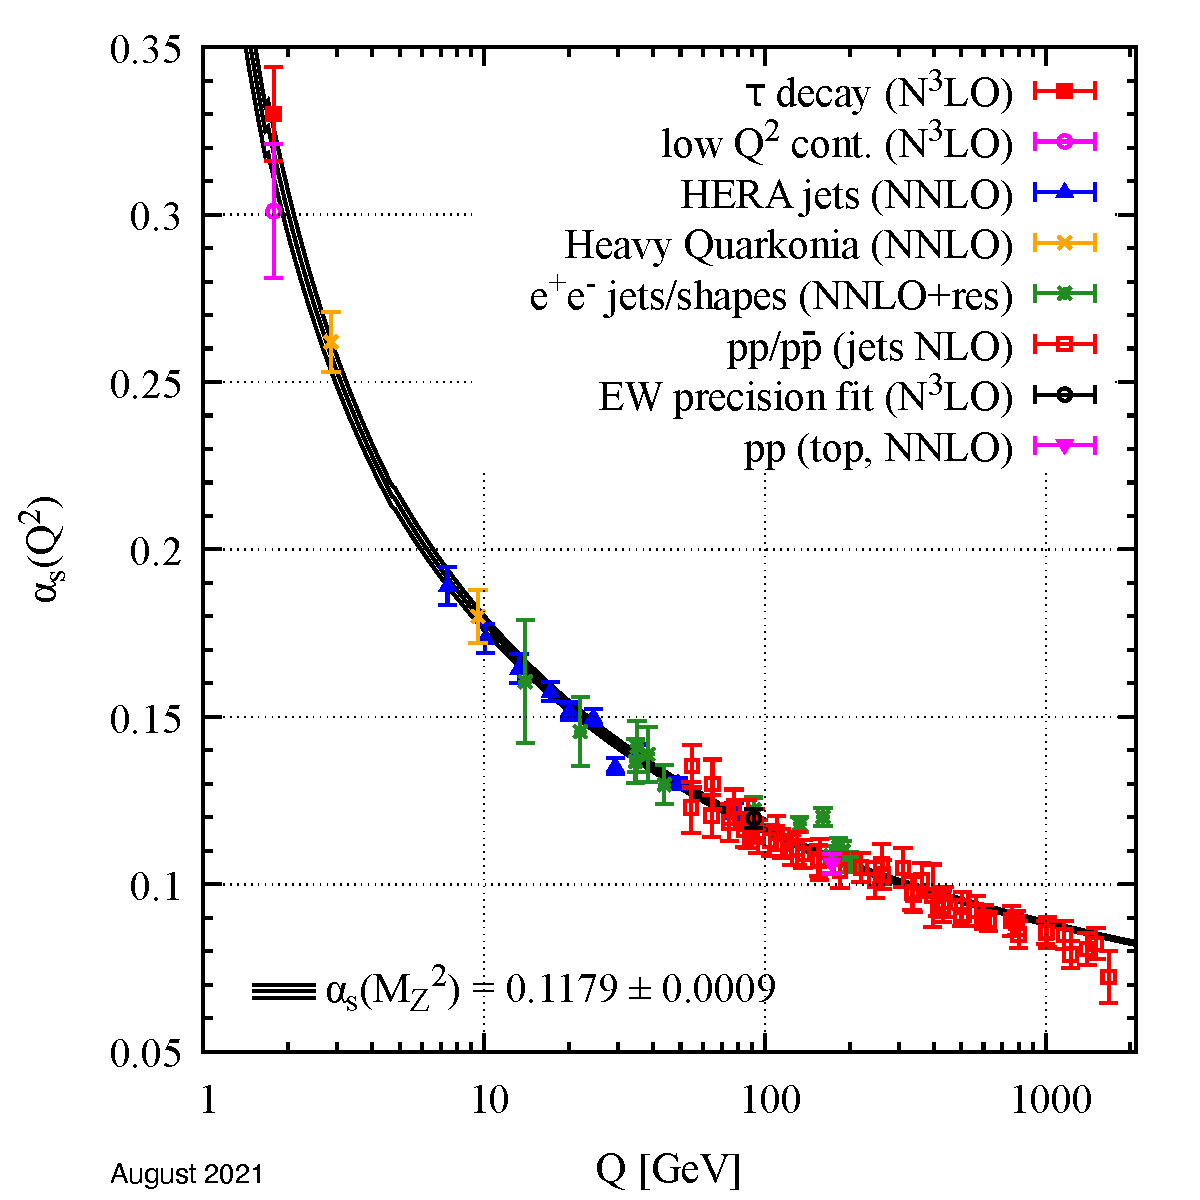
\includegraphics[scale=0.65]{MisImages/alphasVsQ2021.pdf}
    \caption{ The running coupling constant from the experiments as a function of the energy scale Q \cite{alphasVsQ:2022}.}
    \label{fig:alphasvsQ}
\end{figure}

When the $Q^2$ is small (at longer distances), the coupling becomes strong that the perturbative theory is no longer applicable; this region corresponds to the non-perturbative regime. The self-interaction of gluons forms the ``glue tube'' by squeezing the lines of forces together, which implies the quark-antiquark potential of the form $V(r)=-\frac{4}{3}\frac{\alpha_s}{r} + \lambda r$. Because of this linear potential, it requires infinite energy to separate quark and antiquark pair, resulting in the phenomenon called ``confinement". The ``confinement'' suggests that quarks and gluons are confined within the nucleons.   

    


 

\chapter{SPIN STRUCTURE OF PROTON}

\section{Introduction}

A proton is a complex composite structure comprising three quarks: two up ($u$) and one down ($d$). Most of its spin structure comes from sources other than its valence quarks. After the compelling discovery of the EMC collaboration \cite{EuropeanMuon:1987isl}, understanding the proton structure has become challenging for the particle physicist community. While the proton constituents are well understood, their contribution to the proton spin is still puzzling. Despite tremendous development in the experiment and theory of (non-)perturbative QCD, we are not yet able to fully understand how quarks and gluons spin and orbital angular momentum contribute to the proton's spin. 

The knowledge of the proton spin structure is based on annihilation and scattering experiments. In the annihilation experiments, leptons -antileptons - beams are used. When highly energetic lepton and anti-lepton beams collide, they annihilate to form a highly energetic virtual photon (as leptons undergo electromagnetic interaction) enough to generate a quark and antiquark pair rapidly flying apart. As they fly, they are pulled so strongly to store more energy, and in the vicinity of the proton's radius, they break apart radiating gluons, which further fragment into quark and anti-quark pairs. This is called the fragmentation process. This process continues until the energy is compensated for by producing streams of particles in the form of jets. In the process, (anti-)quarks combine to form a stable colorless state  of baryons and mesons, which is called hadronization. Analyzing the jets or exclusive particles along the direction of the initial parton provides information about the partonic structure of the nucleon. 

On the other hand, the scattering experiments used either lepton-proton collision or proton-proton ($pp$) collision. In both cases, enough energy is supplied in the colliding beams such that a quark in the proton gets knocked out and undergoes fragmentation and hadronization process as in the annihilation process producing jets, which serve as a proxy for the partons producing it.  

%definition of PDFs, TMDs, and GPDs
The proton's parton structure is characterized by a parton distribution function (PDF) and fragmentation functions (FFs). These functions provide insight into the distribution of momentum carried by the partons within the proton. Assuming the probed nucleon is moving along the $\hat{z}$ direction, then the extension of longitudinal momentum-dependent PDF can be made in the momentum space or in the coordinate space. The transverse momentum extension to the longitudinal momentum dependence PDF is called the transverse momentum dependent PDFs\cite{Collins:1981uw, Mulders:1995dh, Boer:1997nt, Bacchetta:2006tn}, whereas the extension in the coordinate space is called the generalized parton distributions (GPDs)\cite{Ji:1996ek, Muller:1994ses, Radyushkin:1997ki}. The longitudinal momentum-dependent PDFs, TMDs, and GPDs enable three-dimensional tomography of the proton structure. These distributions not only describe the parton composition within the proton but also links the parton properties from the  strong QCD interactions to the nucleon. 

\section{Leading Twist Transverse Momentum Dependent Distribution Functions}
The PDFs depend on the polarization state of the nucleon and the parton within the nucleon. There exist eight leading-order TMD, whose physical description is listed in Figure \ref{fig:tmdpdfs}. $f_1(x, k_T)$ is the simplest unpolarized TMD, which describes a probability of finding a quark carrying longitudinal momentum $x$ of the nucleon and a transverse momentum $k_T=|\vec{k}_T|$ in a fast-moving nucleon. For an unpolarized nucleon, the transverse quark distribution is given by the Boer-Mulder function, $h_{1}^\perp(x, k_T)$.  If the nucleon is polarized longitudinally to the momentum direction, then the longitudinal quark distribution is given by the helicity PDF $g_{1L}(x, k_T)$ and a transverse distribution is given by Worm Gear $h_{1L}(x, k_T)$. The Sivers function, $f_{1T}^\perp(x, k_T)$, is introduced to describe spin-independent quark distribution in a transversely polarized nucleon. Furthermore, for a transversely polarized nucleon, the longitudinal quark polarization is given by a Worm Gear, $g_{1T}(x, k_T)$, and a transverse quark polarization is given by transversity $h_{1T}(x, k_T)$ or the pretzolosity $h_{1T}^\perp(x, k_T)$. The Sivers, Boer-Mulders, and pretzelosity require orbital angular momentum in the nucleon since they involve a transition between initial and final nucleon states whose orbital angular momentum differs by $\pm 1$ (Sivers and Boer-Moulder) or by $\pm 2$ (pretzelosity). The Worm-gears link two perpendicular spin directions and are also connected to the quark orbital motion inside nucleons \cite{Aidala:2012mv}.

\begin{figure}[H]
    \centering
    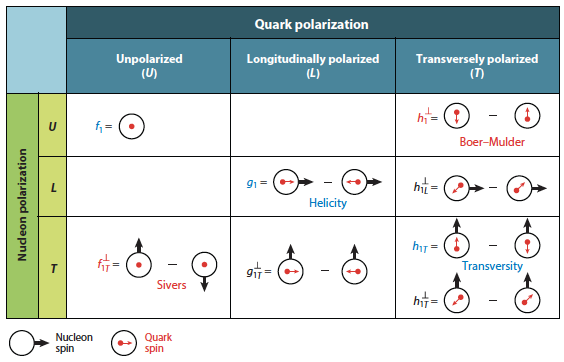
\includegraphics[scale=0.6]{MisImages/Ch2Images/pdfs.png}
    \caption{Leading twist TMDs classified according to the quark polarizations (f, g, h) and nucleon (U, L, T) \cite{Accardi:2012qut}. A similar classification of TMD distributions exists for gluons.}
    \label{fig:tmdpdfs}
\end{figure}
    
The three TMD distributions: $f_1(x, k_T)$, $g_{1L}(x, k_T)$, and $h_{1T}(x, k_T)$, survives upon integration over the $k_T$ as they are even under the exchange of $k_T\rightarrow -k_T$, leading to three collinear PDFs. All the other TMD distributions are $k_T-$odd, which vanishes upon $k_T$ integration. These $k_T-$odd TMDs are beyond the scope of this thesis; Only the leading order TMD distribution functions will be discussed, focusing on the transversity PDF.   

The quest for transverse spin provides a unique way to unravel the proton spin structure. The spin of the proton perpendicular to the proton's momentum direction is a vector that correlates with the transverse component of the parton (TMD) or the transverse position of the parton (GPD). The first observation of the single spin asymmetry (SSA) was in 1976 from  polarized $pp$ data at $\sqrt{s}$=6 GeV and 12 GeV for the charged pions at Argonne National Laboratory Zero Gradient Synchroton \cite{Klem:1976ui}. This observation was supported by similar experiments \cite{Dragoset:1978gg, Antille:1980th, Apokin:1990ik, Saroff:1989gn}. Similar asymmetries have been observed in polarized $pp$ by the RHIC where the asymmetry reaches up to 40\% \cite{Aschenauer:2016our}, lepton-nucleon experiment in at HERMES, COMPASS, and JLab. The observed asymmetry in the hadron production off the polarized nucleon tells us about the spin-orbit coupling in the nucleon and/or in the fragmentation process \cite{Aidala:2012mv}.    

The quantitative understanding of PDFs has been achieved through QCD analysis of an extensive dataset, encompassing experiments such as Deep Inelastic Scattering (DIS), Drell-Yan lepto-production, and inclusive processes in $pp$ collisions \cite{pdfCTEQ:2021, DSSV:2019, Cocuzza:2023oam}.
At the leading twist, the nucleon structure is fully described by three Parton Distribution Functions (PDFs): the unpolarized PDF, $f_1(x)$, the helicity PDF, $g_1(x)$,  and the transversity PDF, $h^q_1(x)$, where $x$ is the nucleon momentum fraction carried by patrons. Although $f_1(x) $ and $g_{1}(x)$ are reasonably well constrained by experimental data \cite{EurPhys,deFlorian:2009vb}, the knowledge of $h_1^{q}(x)$ is limited \cite{Anselmino:2013vqa, Kang:2015msa, Radici:2018iag} to semi-inclusive deep inelastic scattering (SIDIS) \cite{HERMES:2008mcr, HERMES:2009lmz, COMPASS:2008isr, COMPASS:2012bfl, COMPASS:2014bze, JeffersonLabHallA:2011ayy}, $e^+e^-$ \cite{BaBar:2013jdt, Belle:2008fdv} and $p^\uparrow p$ \cite{STAR:2015jkc} data. This is because $h_1^{q}(x)$ is a chiral-odd object, and it needs to be coupled with another chiral-odd partner to form a chiral-even cross section that is experimentally observable.

\section{Current Understanding of the Collinear PDFs}
\subsection{Unpoalrized PDF}
Unpolarized PDF, $f_1(x)$, describes the probability of finding an unpolarized parton within an unpolarized proton as a function. $f_1(x)$ is well constrained by the global QCD analysis of a vast amount of experimental data from the ATLAS, CMS, and LHCb data from the Large Hadron Collider (LHC), HERA I+II combined DIS data, and measurements from the fixed-target data from Fermilab Tevatron $p\bar{p}$ collider by CTEQ \cite{Dulat:2015mca, pdfCTEQ:2021}, MSHT \cite{Harland-Lang:2014zoa, Bailey:2020ooq}, and NNPDF \cite{NNPDF:2017mvq} groups. Figure \ref{fig:cteqpdf} shows the most recent global QCD analysis of $f_1(x)$ as a function of $x$ for the different quark flavors and the gluon from CTEQ collaboration. The higher $x$ region is dominated by the valence quarks, $u$ and $d$, and gluons. The $f_1(x)$ for gluon is scaled down by the factor of 5, and it indicates that the gluons contribute as much as the valence quarks in the valence region and completely dominate in the lower $x$ region. Although the high$-x$ region is well constrained ($0.1<x$), the low-$x$ region is not well understood, which requires much higher center-of-mass energy collision data, and very limited experimental data is available to probe in this region. 
\begin{figure}[H]
    \centering
    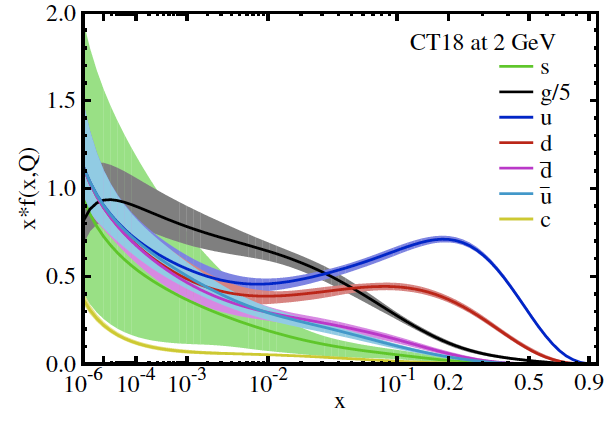
\includegraphics[scale=0.5]{MisImages/Ch2Images/pdfsCT18_fx2GeV.png}
    \caption{Unpolarized PDFs at $Q$ = 2 GeV for $u$, $\bar{u}$, $d$, $\bar{d}$, $s=\bar{s}$, and $g$. The gluon PDF has been scaled down as $g(x, Q)$/5 \cite{pdfCTEQ:2021}.}
    \label{fig:cteqpdf}
\end{figure}

\subsection{Helicity PDF}
The helicity PDF, $g_1(x)$, is defined as the probability of finding a longitudinally polarized parton in a longitudinally polarized nucleon. The $g_1(x)$ for the quarks are mainly constrained by the DIS data. However, the DIS data are less sensitive to the gluons, and polarized $pp$ collision data from RHIC is crucial to probe the gluon polarization. The first evidence of the gluon polarization is established by the global QCD analysis from DSSV14 \cite{DSSV:2014} and confirmed by NNPDF \cite{NNPDF:2017mvq}, and further constrained by DSSV14 \cite{DSSV:2019} utilizing the di-jet measurements from the RHIC \cite{STARdijet:2016, STARdijet:2018}.

Figure \ref{fig:dssv_quark} shows the $g_1(x)$ from DSSV14 for different quark and antiquark flavors, compared to the NNPDFpol1.1. The $u-$quark has a positive helicity, and $d-$quark has negative helicity, meaning that the $u-$quark tends to align its spin along the nucleon polarization, whereas the $d-$quark tends anti-align to the nucleon spin. Helicity PDF for quarks is approaching the precision of the unpolarized. However, the gluon helicity is far from reach to the quark precision level, which is shown in Figure \ref{fig:dssv_gluon}. 
\begin{figure}[H]
    \centering
    \begin{subfigure}{1\textwidth}
    \centering
    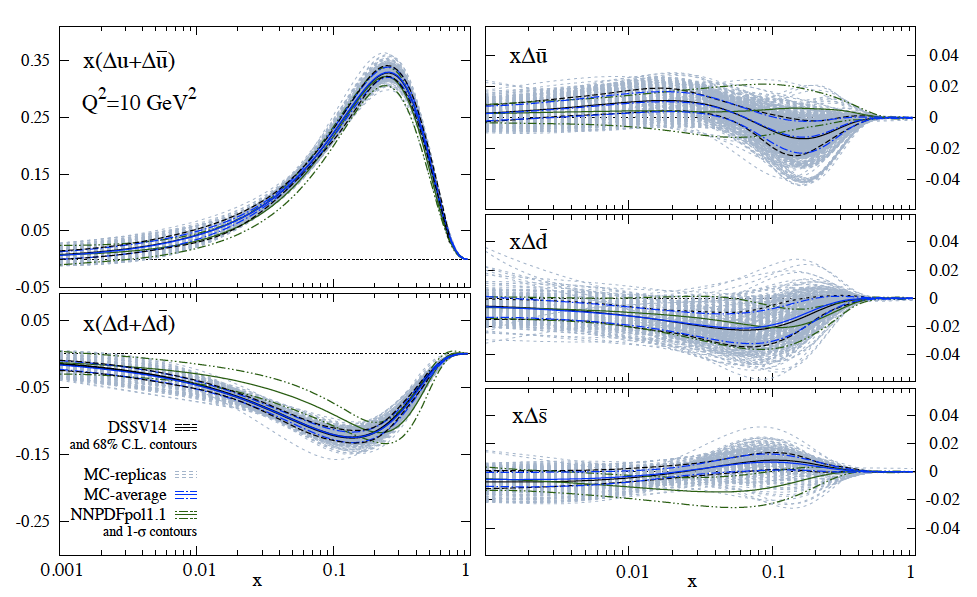
\includegraphics[scale=0.4]{MisImages/Ch2Images/pdfDSSV_gxQ.png}
    \subcaption{Helicity PDFs for the quark and antiquark at $Q^2$ = 10 $\mathrm{GeV^2}$.}
    \label{fig:dssv_quark}
    \end{subfigure}
    \begin{subfigure}{1\textwidth}
    \centering
    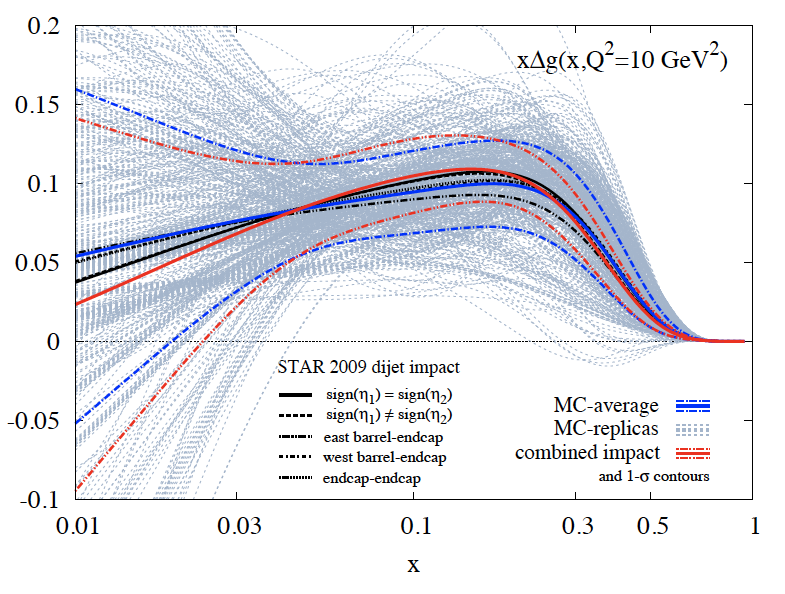
\includegraphics[scale=0.5]{MisImages/Ch2Images/pdfDSSV_gxG.png}
    \subcaption{ Gluon helicity distribution.}
    \label{fig:dssv_gluon}
    \end{subfigure}
    \caption{Helicity PDF for gluon.}
\end{figure}

\subsection{Transversity PDF}
At the leading twist, transversity PDF ($h_1^q(x)$) is defined as the probability of finding a transversely polarized quark in a transversely polarized nucleon, which was first introduced by Ralston and Soper \cite{Ralston:1979}. $h_1^q(x)$  is only a valence quark property and vanishes for the gluon \cite{Barone:2001}. Current understanding of $h_1(x)$ is from global analysis of the SIDIS data from the HERMES \cite{HERMES:2004, HERMES:2008mcr, HERMES:2010} and COMPASS \cite{COMPASS:2008isr, COMPASS:2012bfl, COMPASS:2014bze}, $e^+e^-$ data from Belle \cite{Belle:2008fdv, Belle:2011, Belle:2017} and BABAR\cite{BaBar:2013jdt}, and $pp$ data from STAR \cite{STAR:2015jkc, STAR:2017wsi}. The phenomenological extraction of $h_1(x)$ from these data can be found in Ref. \cite{Kang:2015msa, Radici:2018iag, Cocuzza:2023oam}. 



\begin{figure}[H]
    \centering    
    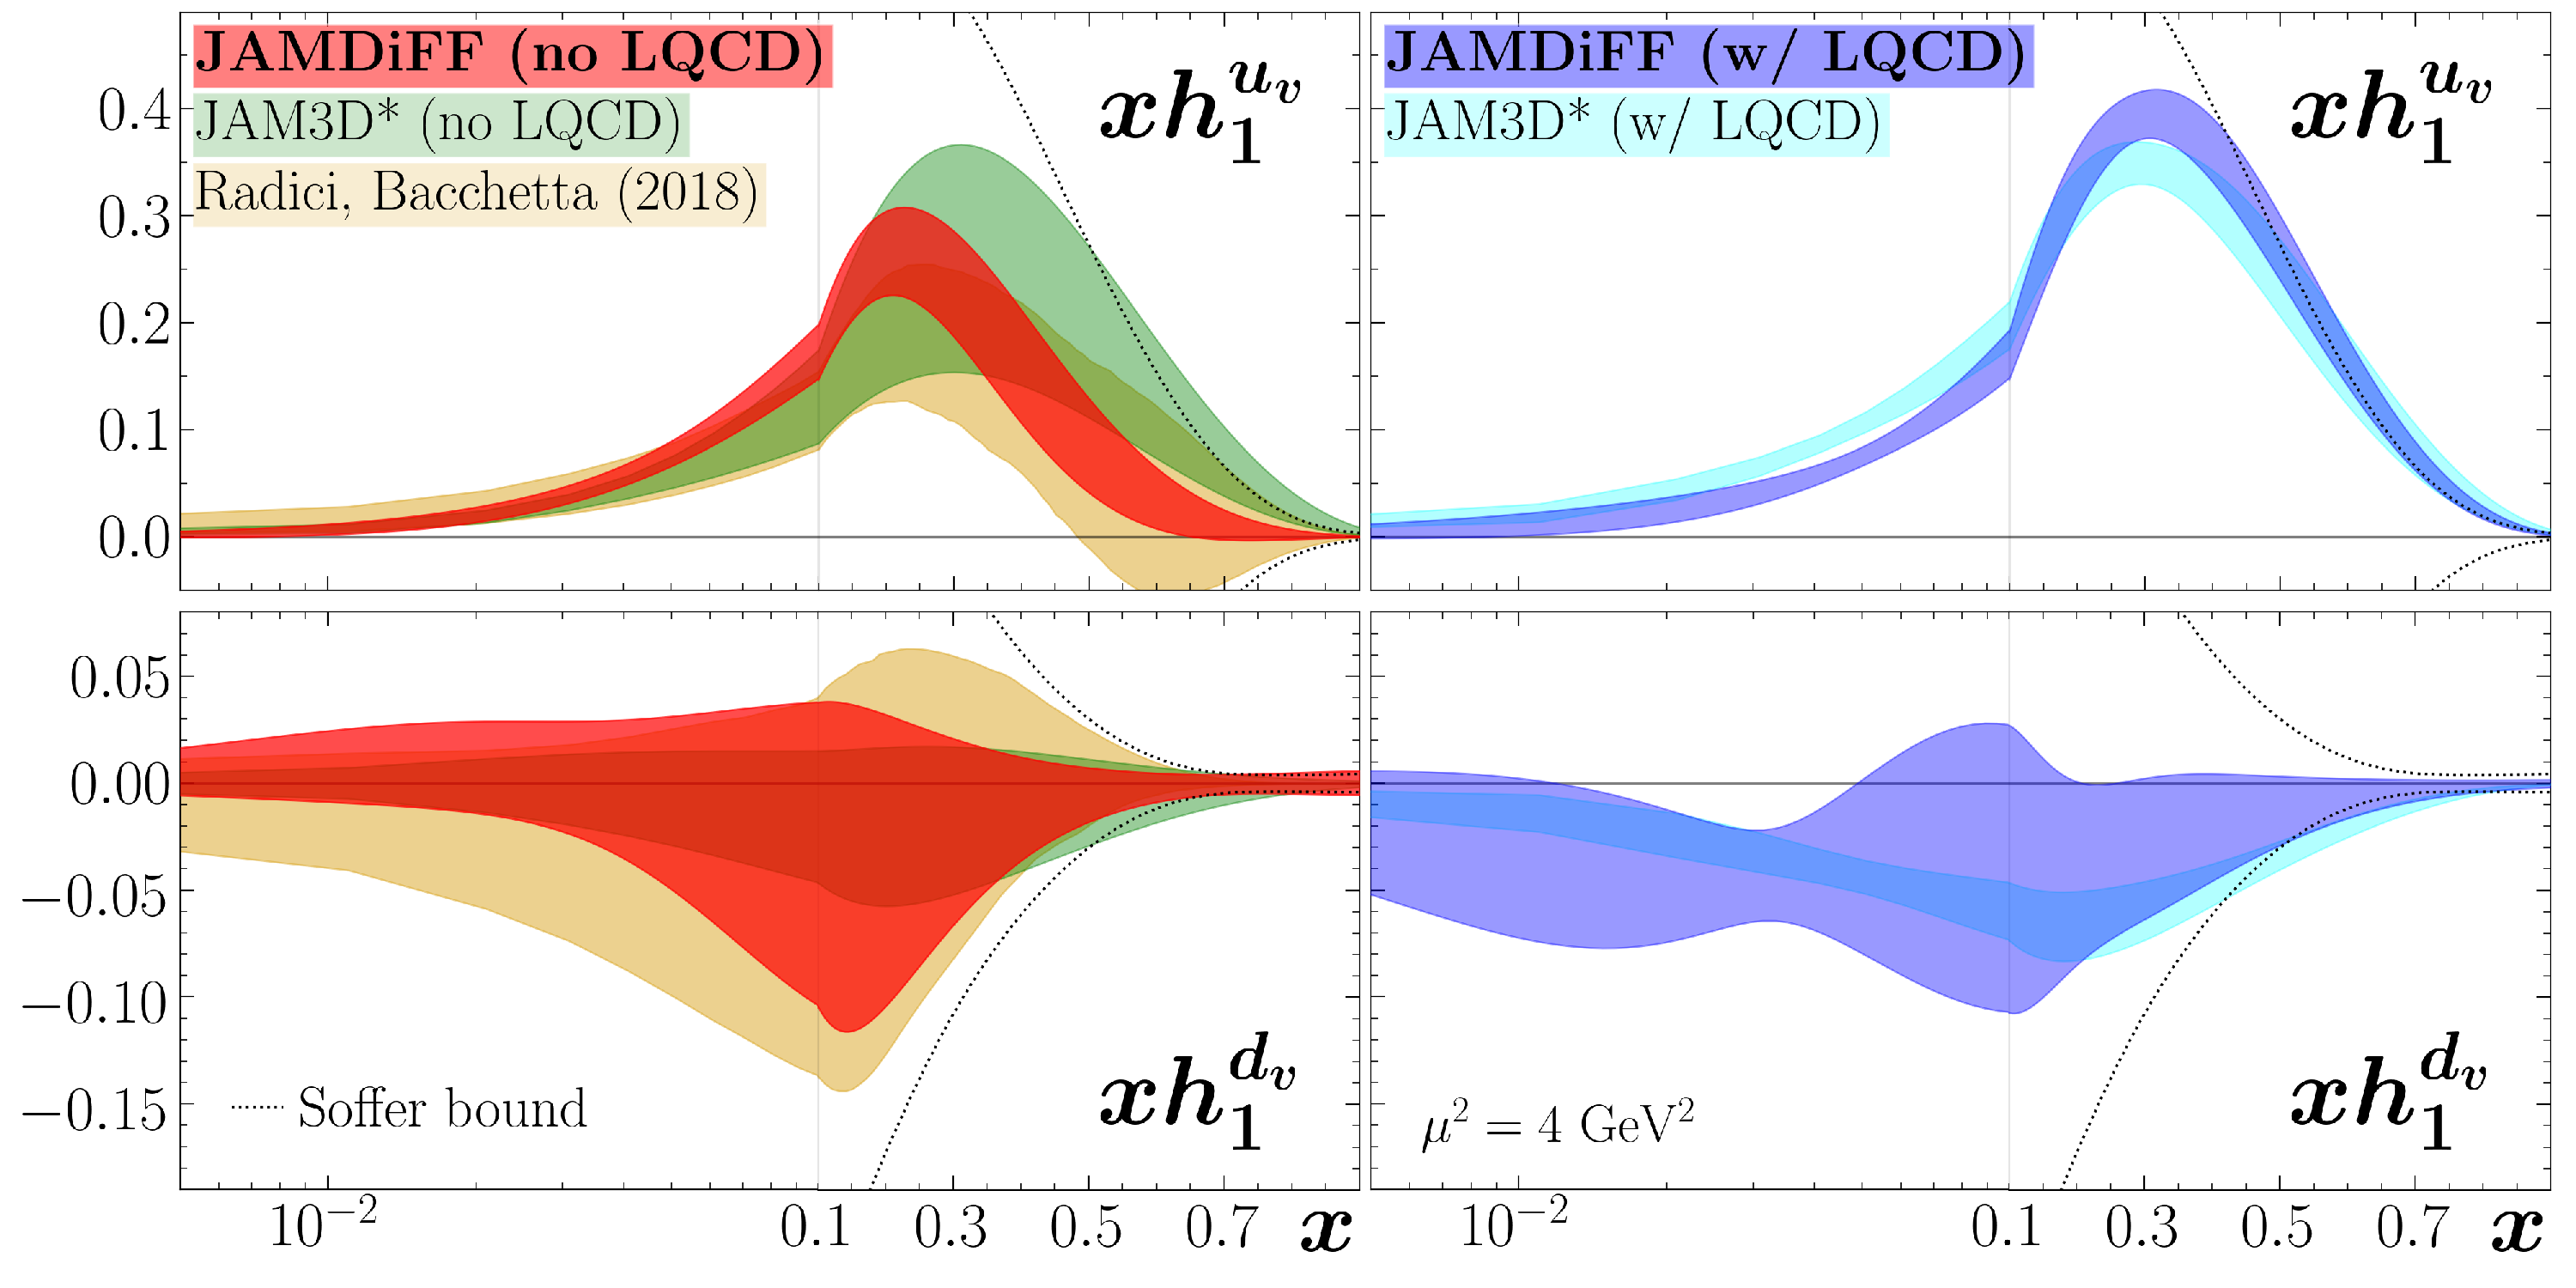
\includegraphics[scale=0.3]{MisImages/Ch2Images/pdfJAM_h1.pdf}
    \caption{Transversity PDF from the JAM collaboration.}
    \label{fig:jamtrans}
\end{figure}

Figure \ref{fig:jamtrans} depicts the recent global extraction of $h_1(x)$ from JAM collaboration \cite{Cocuzza:2023oam}, compared to the extraction from Ref. \cite{Radici:2018iag} (left panel) including the lattice QCD data (right panel) \cite{Gupta:2018, Hasan:2019}. The $h_1(x)$ for the valence quarks feature a similar trend as the $g_1(x)$ but unconstrained by far, even in the valence quark region. The inclusion of the LQCD data, however, appears to constrain significantly.    

\section{Fragmentation Functions}
Fragmentation functions (FFs)  usually appear as a non-perturbative ingredient in the factorization formula when the specific particle species are observed in the final state. FF is defined as the probability of finding  color-neutral particles inside partons. In other words, it describes how color-neutral particles are formed from the colored quarks and gluons.

FF can be studied in single-inclusive hadron production in $e^+e^-$ (SIA), in SIDIS and $pp$ collision processes, where FF frequently appears in the QCD factorized cross section: 
\begin{itemize}
    \item SIA: $\sigma^{e^+e^- \rightarrow hX} = \hat{\sigma}\otimes FF$
    \item SIDIS: $\sigma^{lN \rightarrow lhX} = \hat{\sigma}\otimes PDF \otimes FF$
    \item $pp$: $\sigma^{pp \rightarrow hX} = \hat{\sigma}\otimes PDF \otimes PDF \otimes FF$
\end{itemize}
where $\hat{\sigma}$ represents the process-dependent hard scattering cross section, which is perturbatively calculable, and only the leading order factors are shown. This factorization scheme holds true only if the hard scale is present in each of the processes, such as the center-of-mass energy, $\sqrt{s}$, serves as a hard scale in the SIA, the virtual momentum transfer between lepton and hadron, $Q^2$, serves as a hard scale on the SIDIS, and the transverse momentum of the final state hadron relative to the proton's momentum, $p_{h\perp}$, serves as a hard scale. 

The application of FF was first introduced in the 1970s to explain the observation of large transverse momentum of hadrons in the hadronic collisions from CERN, which could not be explained without including gluonic subprocesses \cite{Metz:2016}. Several FFs appear in the process depending on the inclusion of spin of the hadron and/or parton, transverse momentum of hadron relative to the parton, higher-twist effects, and fragmentation to more than one hadrons, which are summarized in Table \ref{tab:ffs}. 

%TMD fragmentation functions table
\begin{table}[H]
    \centering
    \begin{tabular}{|c|c|c|c|}
    \hline
   \diagbox{H}{q(g)} & U & L (Circ) & T (Lin)  \\
   \hline
    U & $D_1^{h/q(g)}$ & & $H_1^{\perp h/q(g)}$ \\
    \hline
    L &  & $G_1^{h/q(g)}$& $H_{1L}^{\perp h/q(g)}$  \\
    \hline  
    T & $D_{1T}^{\perp h/q(g)}$ & $G_{1T}^{h/q(g)}$ & $H_1^{h/q(g)}$ $H_{1T}^{\perp h/q(g)}$  \\
    \hline     
    \end{tabular}
    \caption{Interpretation of TMD FF for quarks (gluons). }
    \label{tab:ffs}
\end{table}

The $D_1^{h/q(g)}$ is the unpolarized FF, which describes the number density of unpolarized hadrons in an unpolarized quark (gluon). The density of longitudinally polarized hadrons in longitudinally(circularly) polarized quark(gluon) is given by $G_1^{h/q(g)}$. The $H_1^{h/q(g)}$ describes the density of transversely polarized hadron in transversely (linearly) polarized quark(gluon). One should remember that if the parton polarization is involved, then the FF gives the difference in densities, such as $D_1^{h/q(g)}$ has a simple number density interpretation; however, $G_1^{h/q(g)}$ represents the difference in densities of two opposite parton polarization. $H_1^{\perp h}$ is well-known Collins FF \cite{Collins:1992kk}, as it provides access to the transversity in the SIDIS process.


The dihadron FFs (DiFFs) appear in the factorization formula of the processes, where a parton fragments in two hadrons. It is gaining more attention lately because it can be an analyzer for the transversity in the collinear framework, unlike the TMD Collins FF. The DiFFs measure the probability of finding two color-neutral hadrons in a parton. $D_1^{h_1h_2}$ represents the measure of such probability for two hadrons $h_1$ and $h_2$ in an unpolarized parton. Including the transverse momentum of parton $k_T$ and the polarization, the probability density of finding two unpolarized hadrons  in a transversely polarized target is given by two DiFFs: $H_1^{\sphericalangle, h_1h_2}$ and $H_1^{\perp, h_1h_2}$ \cite{Metz:2016}. The $H_1^{\sphericalangle, h_1h_2}$ is a well-studied DiFF than other DiFFs, as it provides access to the transversity, for example, in polarized $pp$ collisions. It is often called the Interference Fragmentation Function (IFF) because it requires interference between different dihadron production channels for its survival \cite{Jaffe:1997hf, Jaffe:1997pv, Bacchetta:2004it}.       

\section{Accessing Transversity Via Dihadron Channel: Theoretical Description}
\label{sec:ifftheory}
 Accessing the transversity PDF, which is chiral-odd, can be quite challenging. This must be combined with another chiral-odd partner to yield a chiral-even cross-section. As a result, it cannot be accessed in inclusive processes. Furthermore, to access transversity, knowledge of another chiral-odd object that needs to appear together is required. This difficulty makes it less straightforward to access than other leading-order parton distribution functions, making it the least understood among other leading-order PDFs.

Transversity can be accessed through a single hadron production, either by exploiting TMD factorization (e.g., Collins effect \cite{Collins:1992} in SIDIS) or collinear sub-leading twist (twist 3) factorization in hadronic collisions \cite{DAlesio:2020vtw, Cammarota:2020qcw}.
 Alternatively, one can consider the unpolarized dihadron production at leading twist collinear factorization, where transversity couples with the interference fragmentation function, $H^\sphericalangle_1$ (IFF) \cite{Tang:1998wp, Jaffe:1997hf, Jaffe:1997pv, Bacchetta:2004it}.
 The collinearity is preserved in this channel as the dihadron center of mass travels along the jet axis, and the IFF survives even after integrating over the transverse momentum of the hadron pair. Moreover, this channel doesn't require a jet reconstruction, devoid of systematic uncertainty associated with the jet reconstruction.  

The discussion will focus solely on accessing transversity through the dihadron channel in $p^\uparrow p$ collision. This specific channel is used to measure the azimuthal correlation asymmetry in this analysis, which can be expressed as,
\begin{equation}
    \label{eq:dihadch}
    p^\uparrow_a(\mathbf{S_a, P_a}) + p_b (\mathbf{P_b}) \rightarrow (h_1 h_2)_{jet} (\mathbf{P_h})  + X,
\end{equation}
where $p^\uparrow_a(p_b)$ is a transversely polarized (unpolarized) proton, $h_1$ and $h_2$ are the final state unpolarized charged hadrons  within a jet, and $X$ represent undetected final state particles. The boldface quantities in the equation are regular three vectors, where $\mathbf{S}$ is the polarization vector and $\mathbf{P}$ is the momentum vector. The final state hadrons could be protons, kaons, or pions.

\drawgraphics{0.8}{Results/IFF2015/ppcol.png}{Dihadron channel in $p^\uparrow p$ showing the fragmentation of polarized parton and final state unpolarized dihadron pair. The respective PDFs and FFs are indicated at where they appear in the process.}{fig:ppcol}

The dihadron channel is depicted schematically in Figure \ref{fig:ppcol}. The polarized (unpolarized) proton originates from the left (right), and the associated kinematic variables are indicated with subscripts $a(b)$. The transversity PDF of a transversely polarized proton $a$ is denoted by $h_1$, while the unpolarized PDF of proton $b$ is denoted by $f_1$. The hard scattering occurs between a transversely polarized parton $i$ from proton $a$ and an unpolarized parton $j$ from proton $b$. The cross section of the hard scattering, denoted as $\hat{\sigma}$, is perturbatively calculable. This scattering occurs at an extremely small distance ($\lesssim 10^{-15}$ m), where the partons are considered asymptotically free. Subsequently, the hard scattered partons undergo fragmentation and hadronizes into color-neutral stable particles. The fragmentation of the polarized scattered parton $k$ is described by the spin-dependent fragmentation function $H^\sphericalangle_1$, while the fragmentation of the unpolarized parton $l$ is described by $D_1$. At the leading twist, these fragmentation functions also possess a probabilistic interpretation, representing the probability of finding color-neutral hadrons within the parton. In the final state, we observe hadrons emerging from the polarized parton $k$, either in the form of jets or exclusively, which grants access to the quark transversity coupled with the IFF.

Measuring two hadrons in the final state provides two vectors associated with the hadron pair, offering a convenient theoretical framework \cite{Bacchetta:2003vn}. If $\mathbf{P_{h_1}}$ and $\mathbf{P_{h_2}}$ represent the momenta of the two hadrons, these vectors can be defined as follows:

\begin{equation}
\mathbf{P_h} = \mathbf{P_{h_1}} + \mathbf{P_{h_2}},\ \mathrm{and}\ \mathbf{R} = \mathbf{\frac{P_{h_1} - P_{h_2}}{2}},
\end{equation}

Here, $\mathbf{P_h}$ denotes the resultant momentum of the hadrons, and $\mathbf{R}$ represents the relative momentum vector. Due to the presence of the relative momentum vector $\mathbf{R}$, the IFF can be integrated over the transverse component of $\mathbf{P_h}$ with respect to the jet axis. Additionally, the transverse component of the fragmenting quark can be expressed in terms of the transverse component of the relative momentum, denoted as $\mathbf{R_T}$, through the mixed product $\mathbf{S \cdot R \times P_h}$. In this channel, the center of mass of the hadron pair moves collinearly with the jet axis, thereby preserving the concept of collinear factorization; hence the jet reconstruction is not required.
For a dihadron channel given by equation \ref{eq:dihadch}, only one type of asymmetry, $A_{UT}$,  exists, which is given by, 
    \begin{equation}
        \label{eq:asymxsec}
        A_{UT} = \frac{d\sigma^\uparrow - d \sigma^\downarrow}{d\sigma^\uparrow + d \sigma^\downarrow} \equiv \frac{d\sigma_{UT}}{d\sigma_{UU}},
    \end{equation}
where $d\sigma_{UT}$ is the difference between the cross section when the polarized proton $a$ is polarized up ($\uparrow$) and down ($\downarrow$), whereas $d\sigma_{UU}$ is the unpolarized cross section. The polarized and unpolarized part of the cross section can be expressed as \cite{Bacchetta:2004it}, 

\begin{align}
\label{eq:xsecut}
    d\sigma_{UT} &= 2|\mathbf{P_{h\perp}}|\sum_{i,j,k,l} |\mathbf{S_a}|\ sin(\phi_S - \phi_R)  \int \frac{dx_a dx_b}{8\pi^2 z_h} f_1^{j/b}(x_b)\ h_1^{i/a}(x_a)\ \frac{d\Delta\sigma^{i^\uparrow j \rightarrow k^\uparrow l}}{d\hat{t}} \nonumber \\
     & \times \frac{\mathbf{R}}{M_h}\ sin\theta \ H_1^{\sphericalangle,h_1h_2/k}(z_h, cos\theta, M_h^2)
\end{align}
\begin{align}
\label{eq:xsecuu}
    d\sigma_{UU} &= 2|\mathbf{P_{h\perp}}|\sum_{i,j,k,l} \int \frac{dx_a dx_b}{8\pi^2 z_h} f_1^{i/a}(x_a)\ f_1^{j/b}(x_b)\ \frac{d\Delta\sigma^{ij \rightarrow kl}}{d\hat{t}} \times  D_1^{h_1h_2/l}(z_h, cos\theta, M_h^2)
\end{align}
In the equations above, $|\mathbf{P_{h\perp}}|$ represents the magnitude of the transverse component of $\mathbf{P_h}$ with respect to the beam direction. This component serves as a hard scale for the process. The PDFs $f_1$ and $h_1$ correspond to the unpolarized and transversity PDFs, respectively. $H_1^{\sphericalangle h_1h_2}$ denotes the IFF, while $D_1^{h_1h_2}$ represents the unpolarized counterpart of the IFF.

The definitions of the azimuthal angles $\phi_S$ and $\phi_R$ are derived from Figure \ref{fig:angles} and are given by Equations \ref{eq:cosang}-\ref{eq:sinang}. These angles are defined in the center of mass of the hadronic system. Specifically, $\phi_S$ denotes the angle between the scattering plane formed by $\mathbf{P_a}$ and $\mathbf{P_h}$, and the polarization vector $\mathbf{S_a}$. On the other hand, $\phi_R$ represents the angle between the scattering plane and the dihadron plane formed by the momenta $\mathbf{p_{h_1}}$ and $\mathbf{p_{h_2}}$.

The hard scale is assumed to exceed the dihadron system's proton mass significantly and the invariant mass, denoted as $M_h$. The validity of the assumptions holds only at the leading twist (leading order in $1/|\mathbf{P_{h\perp}}|$).
\begin{equation}
    \label{eq:cosang}
    cos \phi_S = \frac{\hat{P_a}\times \mathbf{P_h}}{|\hat{P_a}\times \mathbf{P_h}|}\cdot \frac{\hat{P_a}\times \mathbf{S_a}}{|\hat{P_a}\times \mathbf{S_a}|}, \hspace{2em}     cos \phi_R = \frac{\hat{P_h}\times \mathbf{P_a}}{|\hat{P_h}\times \mathbf{P_a}|}\cdot \frac{\hat{P_h}\times \mathbf{R}}{|\hat{P_h}\times \mathbf{R}|} 
\end{equation}
\begin{equation}
    \label{eq:sinang}
sin \phi_S = \frac{(\mathbf{P_h}\times \mathbf{S_a})\cdot \hat{P_a}}{|\hat{P_a}\times \mathbf{P_h}||\hat{P_a}\times \mathbf{S_a}|}, \hspace{2em} sin \phi_R = \frac{(\mathbf{P_a}\times \mathbf{R})\cdot \hat{P_h}}{|\hat{P_h}\times \mathbf{P_a}||\hat{P_h}\times \mathbf{R}|}
\end{equation}

The polarized cross section exhibits a sinusoidal modulation of the azimuthal angle $\phi_{RS}$ (defined as $\phi_S - \phi_R$), while such modulation is suppressed in the unpolarized cross section. This observation indicates a bias in the dihadron yields within the specific $\phi_{RS}$ bin, resulting in an asymmetry that arises solely from polarization effects. By utilizing Equations \ref{eq:xsecut} and \ref{eq:xsecuu}, Equation \ref{eq:asymxsec} can be expressed as follows:

\begin{equation}
A_{UT}^{sin\phi_{RS}} = \frac{1}{|\mathbf{S_a}|}\frac{d\sigma^\uparrow - d\sigma^\downarrow}{d\sigma^\uparrow + d\sigma^\downarrow},
\end{equation}

This equation isolates $A_{UT}$ as the amplitude of the "sine" modulation of dihadron yields in $\phi_{RS}$ at the leading twist. To represent the asymmetry associated with the "sine" modulation in $\phi_{RS}$, it will henceforth be denoted as \aut. Experimental measurement of \aut\ involves counting the number of dihadrons in $\phi_{RS}$ bins for both beam polarizations ($\uparrow$ and $\downarrow$), which is sensitive to the product $h_1 H^\sphericalangle_1$:

\begin{equation}
A_{UT} \propto \sum_{i,j,k,l} \frac{f_1^{j/b}(x_b) h_1^{i/a}(x_a) H_1^{\sphericalangle h_1h_2/k}(z_h,M^2_h) }{f_1^{j/b}(x_b) f_1^{i/a}(x_a) D_1^{h_1h_2/l}(z_h, M^2_h)},
\end{equation}

Here, all components are non-perturbative objects, and precise experimental knowledge is required to extract transversity. The unpolarized PDF is known to have higher precision based on SIDIS data \cite{H1:2015ubc}, and the IFF has limited knowledge from the $e^+e^-$ experiments. However, the unpolarized Fragmentation Function (FF) $D_1^{h_1h_2}$ lacks experimental constraints, and the global extraction of transversity relies on simulations, leading to large model-dependent uncertainties. To constrain $D_1$ and, consequently, transversity, it is crucial to experimentally measure $d\sigma_{UU}$, an observable discussed in Chapter \ref{chapter:xsec} that is of great importance.

\drawgraphics{0.7}{ImgIFF/geom.png}{The azimuthal angle definitions in the dihadron channel.}{fig:angles}

The relative partial wave expansion of FFs in the  cross sections $d\sigma _{UT}$ and $d\sigma_{UU}$ using the basis of Legendre polynomials through the cos$\theta$ dependence provides intriguing physics insight \cite{Bacchetta:2002ux}. Keeping up to $L=1$, we have,
\begin{equation}
D_1(z, cos\theta, M^2_h)\rightarrow D_{1,oo}(z,M_h^2)+ D_{1,ol}(z,M_h^2) cons\theta + D_{1,ll}(z,M_h^2)\frac{1}{4}(cos^2\theta -1)
\end{equation}
\begin{equation}
sin\theta H_1^\sphericalangle(z, cos\theta, M^2_h)\rightarrow H_{1,ot}^\sphericalangle(z, M^2_h)sin\theta+ H_{1,lt}^\sphericalangle(z, M^2_h)sin\theta cos\theta
\end{equation}
In this context, the double-index notation is used to describe the polarization state in the center of mass of the dihadron for each specific probability amplitude. For instance, $D_{1, oo}$ corresponds to the decay into a $L=0$ pair (s-wave), while $D_{1,ol}$ refers to the interference between the decay amplitudes of a $L=0$ pair and a $L=1$ pair (s-p interference) polarized longitudinally along the center of mass of $\mathbf{P_h}$. Similarly, $H_{1,ot}^\sphericalangle$ represents the interference between the decay amplitudes of a $L=0$ pair and a transversely polarized $L=1$ pair. Furthermore, $H_{1, lt}$ and $D_{1, ll}$ denote the interference between decay amplitudes at different polarization states of $L=1$ pairs.

The $p$-wave contribution arises from the spin-1 resonance in the dihadron production channel. As a result, the $p$-wave fragmentation functions (FFs) ($ll$ or $lt$ terms) exhibit a characteristic mass dependence, with a distinct resonance peak around the mass of the $\rho$ meson ($\sim 0.77$ GeV/$c^2$). On the other hand, the interference terms ($ol$ or $ot$ terms) require the presence of both $s$- and $p$-wave channels. Therefore, the intrinsic FFs are expected to be significant near the $\rho$ meson mass region \cite{Jaffe:1997hf, Bacchetta:2002ux, Bacchetta:2004it}.

\section{Experimental Data for DiFFs}
From the discussion in \ref{sec:ifftheory}, it is clear that independent measurement of $H_1^{\sphericalangle h_1h_2}$
and $D_1^{h_1h_2}$ with $z$ and $M_h$ dependence is required to decouple transversity from the $h_1H_1^\sphericalangle$. 

The recent Belle measurements of $\pi^+\pi^-$ cross section differential in $M_h$ and $z$ \cite{Belle:2017} provide crucial observable for the $D_1^{h_1h_2}$ for quarks. However, these measurements are less sensitive to gluon fragmentation. The measurement from the $pp$ data is required to probe gluon fragmentation. 
The unpolarized $\pi^+\pi^-$ cross section measurement in $pp$ collision data from the STAR experiment (Chapter \ref{chapter:xsec}) will fulfill the dire need of this observable for the first time. Belle also measured back-to-back dihadron single spin asymmetry (SSA) sensitive to the spin-dependent IFF \cite{Belle:2011}. The measured SSA is proportional to the product $H_1^\sphericalangle \bar{H_1^\sphericalangle}$. 

The SSA to probe the transverse spin-dependent IFF was measured in the transversely polarized proton target by the HERMES experiment for the first time\cite{HERMES:2008mcr} followed by the COMPASS experiment with the polarized proton and deuteron target \cite{COMPASS:2014ysd} in SIDIS. The COMPASS SSA is of higher precision than the HERMES, showing enhancement around the $\rho-$meson mass ($\sim 0.8$ GeV/$c^2$). 

In polarized $pp$, the STAR experiment reported the first observation of SSA \cite{STAR:2015jkc}, followed by higher precision measurement \cite{Landry:2016} at $\sqrt{s}$ = 200 GeV, which is sensitive to the product $h_1H_1^\sphericalangle$. These measurements also depict the distinct resonance feature consistent with the SIDIS measurements. Similar measurements from STAR at $\sqrt{s}$ = 500 GeV \cite{STAR:2017wsi} observed significant asymmetry peaked around the $\rho-$mass, implying the universality of the physical process involved in the resulting SSA. 







\chapter{EXPERIMENTAL ASPECT}

\section{Relativistic Heavy Ion Collider (RHIC)}
This dissertation is a part of research conducted at the relativistic heavy ion collider (RHIC) at Brookhaven National Lab (BNL), located at Upton, New York, United States. RHIC is the world's first collider, which can collide polarized proton beams up to center-of-mass energy of $\sqrt{s} =$ 510 GeV. It can also collide heavy ion particles of varying energy up to $\sqrt{s} =$ 200 GeV. The detailed overview of the RHIC complex and its components are discussed in reference \cite{Alekseev:2003sk}. Relevant components of the RHIC that have a direct impact on this analysis are discussed in this section.   

\drawgraphics{1}{ExperimentalAspect/Rhic\_complex.png}{Relativistic heavy ion collider complex \cite{rhic}.}{fig:rhic}
   
\subsection{Siberian Snakes and Spin Dynamics}
\label{subsec:snakes}
In high-energy particle colliders, it is important to understand the evolution of the spin of the highly accelerated colliding beam and the tools that control it.  
For a circular accelerator as RHIC, the spin evolution in the external magnetic field is given by the Thomas-BMT equation \cite{Thomas:1927yu, Bargmann:1959gz},
\begin{equation}
    \frac{d\vec{P}}{dt} = -(\frac{e}{\gamma m})[G\gamma \vec{B}_\perp + (1+G)\vec{B}_\parallel]\times \vec{P},
\end{equation}
where $\vec{P}$ is the polarization vector expressed in the frame that moves with the particle. $G(=1.7928)$ is the anomalous magnetic moment of the proton and $\gamma = E/m$. $G\gamma$ is called the spin tune $\nu_{sp}$, which gives the number of full spin precessions in every full revolution. The value of the $\nu_{sp}$ can reach up to 478 at the RHIC top beam energy of 250 GeV. 

It isn't easy to maintain the polarization of the highly accelerated beam in the circular path. Two resonances cause the depolarization; one is due to the misalignment and magnet errors called ``imperfection resonances", and the other is called ``intrinsic resonances," caused by the focusing magnetic fields. The imperfection resonances occur when $\nu_{sp}=G\gamma = n$, where $n$  is an integer. In contrast, the intrinsic resonance occurs when $\nu_{sp} = G\gamma = kP \pm \nu_y$, where $k$ is an integer, $\nu_y$ is the vertical betatron tune, and $P$ is the superperiodicity. These resonances cause the spin of the polarized beam to be fully flipped (slowly accelerated beam) or partially flipped (highly accelerated beam), which are traditionally overcome using a betatron jump. At RHIC, ``Siberian Snake" is used to maintain the stable beam polarization, which can produce a 180\textdegree \ spin rotation about the horizontal axis, which is greater than the spin rotation due to the depolarization resonances. These Siberian snakes are constructed either by using a solenoidal magnet or a sequence of interleaved horizontal and vertical dipole magnets producing local orbit distortion. A full snake is used; however, for a low-energy accelerator, a partial snake suffices to maintain stable beam polarization overcoming the depolarization resonances. 

\subsection{Polarized Proton Injector}
The RHIC polarized beam requires a bunch intensity of $2\times 10^{11}$ protons per bunch. To meet this requirement, the alternating gradient synchrotron (AGS) needs to reach bunch intensity of $4\times 10^{11}$ to allow room for some losses while transferring it to the RHIC rings. The optically pumped polarized ion source (OPPIS) produces a polarized $H^-$. It produces 500 $\mu A$ in a single  300 $\mu s$ pulse, which corresponds to the $9\times 10^{11}$ polarized $H^-$. The polarized $H^-$ ions are accelerated to 200 MeV with a radio frequency quadruple (RFQ) and 200 MHz LINAC with an efficiency of about 50\%. The pulse of $H^-$ ions is strip-injected and captured in the AGS Booster as a single bunch, containing $4\times 10^{11}$ polarized protons. Each polarized proton bunch is accelerated to the Booster to 1.5 GeV kinetic energy and transferred to the AGS, which is accelerated to 25 GeV. Finally, the beam bunches are handed to the RHIC rings for further acceleration to 100 or 250 GeV.     


\subsection{Acceleration in the Booster and the AGS}
The polarized proton bunch in the AGS may lose its polarization due to the  depolarization resonances. This is overcome by installing a partial (5\%) Siberian snake at one of the straight sections of the AGS, which is sufficient to avoid any depolarization due to imperfection resonances. The acceleration and beam transfer efficiency is greater than 50\%, giving $2\times 10^{11}$ protons per bunch. This process is repeated until all 120 bunches of the RHIC ring are filled. 

\subsection{RHIC Rings General Layout}
Two full Siberian Snakes on the opposite side of each RHIC ring opposite side serve to avoid depolarization from imperfection and intrinsic depolarization resonances up to the top energy of 250 GeV. These Siberian Snakes introduce a 180\textdegree\ spin rotation around the horizontal axis  without generating a net orbit distortion. In addition, the two axes of the two Snakes in each ring must be perpendicular. Moreover, Snakes are installed in the exact opposite direction in the ring; in fact, the beam direction in one snake should be exactly opposite. Two pairs of Snakes, one pair in each ring, are installed at the 3 and 9 o'clock sections of the RHIC as shown in figure \ref{fig:rhic}.

To achieve the desired beam polarization at the interaction region, a set of two pairs of spin rotators, two sets of that one for the STAR and the other for the PHINIX, are installed right before and after the interaction region. The equilibrium position of the beam polarization is the transverse direction. Whenever a longitudinal polarization is needed, the spin rotators before the interaction rotates the beam polarization to the longitudinal direction, and the rotators beyond the interaction point bring it back to the transverse direction. Having its own set of spin rotators for the STAR and PHENIX experiments allowed an independent choice of beam polarization simultaneously.   

\subsection{Polarimetry}
Measuring the beam polarization with higher precision at RHIC is crucial, as the polarization value normalizes many spin physics analyses. There are two proton-carbon (pC) Coulomb Nuclear Interference (CNI) \cite{KURITA2003C356}, one in each ring, for the relative polarization measurement, and one hydrogen gas jet (H-jet) polarimeter \cite{Zelenski:2005mz} at one of the interaction points for the absolute polarization. 

The pC CNI polarimeter uses a very thin ribbon of carbon targets developed by IUCF, which is simpler and easy to handle in the vacuum than the H-jet CNI. The analyzing power of pC CNI is about 3-5\% for an elastic scattering in the small angle CNI region with a larger cross section being weakly energy dependent over the RHIC energy range from 24 GeV/$c$ to 250 GeV/$c$—the carbon target results in the high luminosity required for fast polarization measurements. The sizeable analyzing power, larger cross section, and the advantages of the solid carbon target make this process ideal for a fast primary RHIC polarimetry.   

The H-jet CNI polarimeter is located at the IP-12 in the RHIC ring, which is close to the pC CNI polarimeter, as shown in figure \ref{fig:rhic}. It is used for the absolute polarization measurement based on the elastic $pp$ scattering in the CNI region. It consists of three parts: the polarized atomic beam source (ABS), the scattering chamber, and the Breit-Rabi polarimeter \cite{Baumgarten2002}. With the state-of-art of ABS, the thickness of the H-jet target is $\sim 10^{12}$ atoms/$cm^2$. The  polarimeter target is free from the atomic beam, which crosses the RHIC beam in the vertical direction. Because of the particle identity, the beam polarization can be directly expressed in terms of the proton target polarization, which is directly measured by the Briet-Rabi polarimeter. Since it is remotely located, there is minimal interference with the other experiments, and it excludes the background generations for the other experiments.   

\section{STAR Detector and Sub-Systems}
The solenoidal tracker at RHIC (STAR) is one of the two large detectors constructed at the six o'clock position in the RHIC complex at Brookhaven National Laboratory (BNL). It is constructed to investigate the behavior of strongly interacting matter at high energy density and to search for the signatures of quark-gluon plasma formation. Moreover, the polarized proton-proton collision program opened up multiple opportunities for the spin physics study of the quarks and gluon in a proton. STAR can measure a hadron production over a large solid angle, featuring detector systems for high-precision tracking, momentum analysis, and particle identification. In addition, large acceptance of the STAR allows event-by-event characterizations of heavy ion collisions and detection of a hadron in jets.

\drawgraphics{0.8}{ExperimentalAspect/STARdet.jpg}{Perspective view of the STAR detector, with a cutaway for viewing inner detector systems.}{fig:stardet}


\drawgraphics{1}{ExperimentalAspect/StarDetCutaway.jpg}{Cutaway side view of the STAR detector \cite{Sakuma2010}.}{fig:starcs}

Figure \ref{fig:stardet} displays the STAR detector layout with a cutaway revealing the inner detector systems. The STAR detector system, cylindrical in shape, includes multiple detectors working in unison. The interaction point is at the center of the detector system, where the closest detector to it is the Silicon Vertex Tracker (SVT) \cite{STAR:2002bzu}. The SVT spans $|\eta|\leq 1$ in pseudorapidity with full azimuthal coverage ($\delta\phi=2\pi$), which provides charged particle tracking, precision localization of the primary vertex, and identification of secondary vertices from the weak decays, for example, $\lambda$, $\Xi$, and $\Omega$s. The Time Projection Chamber \cite{Anderson:2003ur}, which is the heart of the STAR detector system, provides charged particle tracking, Particle Identification (PID), and momentum reconstruction using a 0.5T field from the solenoidal magnet \cite{STAR:1992kiw}. The details of the TPC are discussed in section \ref{subsec:tpc}. The charge particle tracking in the forward region is provided by the Forward TPC (FTPC) \cite{Ackermann:2002yx}, which has a coverage of $2.5 <\eta < 4$ in pseudorapidity with complete azimuthal coverage and symmetry. Moreover, the PID capability of the STAR is extended in the central region ($|\eta|<0.3$) by installing the ring imaging Cherenkov (RICH) detector \cite{STAR:2002aln}. The RICH provides PID of pions and kaons up to $\sim 3$ GeV/$c$, and that for protons up to $\sim 5$ GeV/$c$. In addition, a Time of Flight (TOF) \cite{STAR:tof} detector vastly improves STAR PID by providing the timing information with the same coverage as the TPC in $\eta$ and $\phi$, which is discussed in section \ref{subsec:tof}.    
The STAR event triggering system is based on the transverse energy of the events measured by the electromagnetic calorimeter in the barrel region (BEMC) \cite{STAR:2002ymp} and in the endcap region  (EEMC)\cite{STAR:2002eml}. The BEMC and EEMC have a $-1<\eta<2$ coverage in pseudorapidity and whole $2\pi$ azimuthal angle.


\subsection{TPC and Magnet}
\label{subsec:tpc}
Figure \ref{fig:tpc} shows the schematic view of the STAR TPC. It's cylindrical, measuring 4 meters long and 4.2 meters in diameter. Its acceptance covers $|\eta|\leq 1.8$ in pseudorapidity and full $2\pi$ coverage in azimuth over a full range of multiplicities, which makes it one of the largest operating TPC in the world. It sits in a large solenoidal magnet that operates in a 0.5 T magnetic field. It consists of a thin conductive Central Membrane (CM) at its center, which is 70 $\mu$m thick carbon-loaded Kapton film with a surface resistance of 250 \si{\ohm} per square that operates at 28 kV potential, with the end caps at the ground  providing a uniform electric field of 135 V/cm. The proper boundary conditions between the CM, end caps, and field cage cylinders establish the uniformity of the electric field. The field cage cylinders, inner field cage, and outer field cage, shown in figure \ref{fig:tpc}, provide a series of equipotential rings that divides the space between the CM and the anode planes into 182 equally spaced segments. One ring is common to both sides, where the CM sits. The uniform gradient between the CM and the grounded end caps is maintained by biasing these rings with a chain of precision resistors  of 2 M\si{\ohm}.

   \drawgraphics{1}{ExperimentalAspect/StarTPC.eps}{STAR time projection chamber.}{fig:tpc}

The empty volume between the field cages is filled by the P10 gas, which is 10\% methane and 90\% argon at 2 mbar coverage above atmospheric pressure \cite{Kotchenda:2002rqz}. The P10 gas attributes the fast drift velocity, peaking at a low electric field, which provides the stable drift velocity of the particles insensitive to the variation in the atmospheric conditions, temperature, and pressure.  

The STAR experiment uses the TPC as the primary tracking device, which records particle tracks, measures particle momenta, and identifies the particles by measuring their ionization energy loss ($dE/dx$). It effectively separates pions and protons up to 1.2 GeV/c; however, separating high-energy particles is difficult as the dE/dx becomes less mass dependent at higher energies. As the primary ionizing particles enter the TPC gas volume, their paths are reconstructed with high precision from the released secondary electrons, which drift in the electric field to the readout end caps at the end of the chamber. The TPC performance relies heavily on the magnetic field as electrons may diffuse in the transverse direction, directly impacting particle track reconstruction. The momentum resolution for most of the tracks in the TPC reaches the value of $\delta p/p = 0.02$. The relative momentum resolution increases for a low-momentum track with more hits points along the track. 

The electric and magnetic fields in TPC are uniform all around, radially as well as longitudinally. However, the non-uniformities and global misalignment of the electric and magnetic fields can cause distortions in the position of the secondary electrons reaching the readout pads. One of the causes of the field distortion in TPC is the space charge which occurs due to the piling-up of slow drifting positively charged ions in the gas from the standard operation of the TPC \cite{VanBuren:2005qg}. The effect is propagated to the recorded tracks, corrected by the well-established space charge and grid leak calibration procedure. 

\subsection{Barrel Electromagnetic Calorimeter (BEMC)}
\label{subsec:bemc}
The schematic view of the Barrel Electromagnetic Calorimeter (BEMC)\cite{STAR:2002ymp} is shown in figures \ref{fig:bemcxsec} (cross section view) and \ref{fig:bemcside} (side view). The BEMC sits underneath the aluminum coil of the solenoid covering the $|\eta|\leq 1$ and $2\pi$ in azimuth at a radial distance of about 220 cm from the beam axis matching the coverage of the TPC acceptance. 

\begin{figure}
\begin{subfigure}{0.8\textwidth}
\centering     
    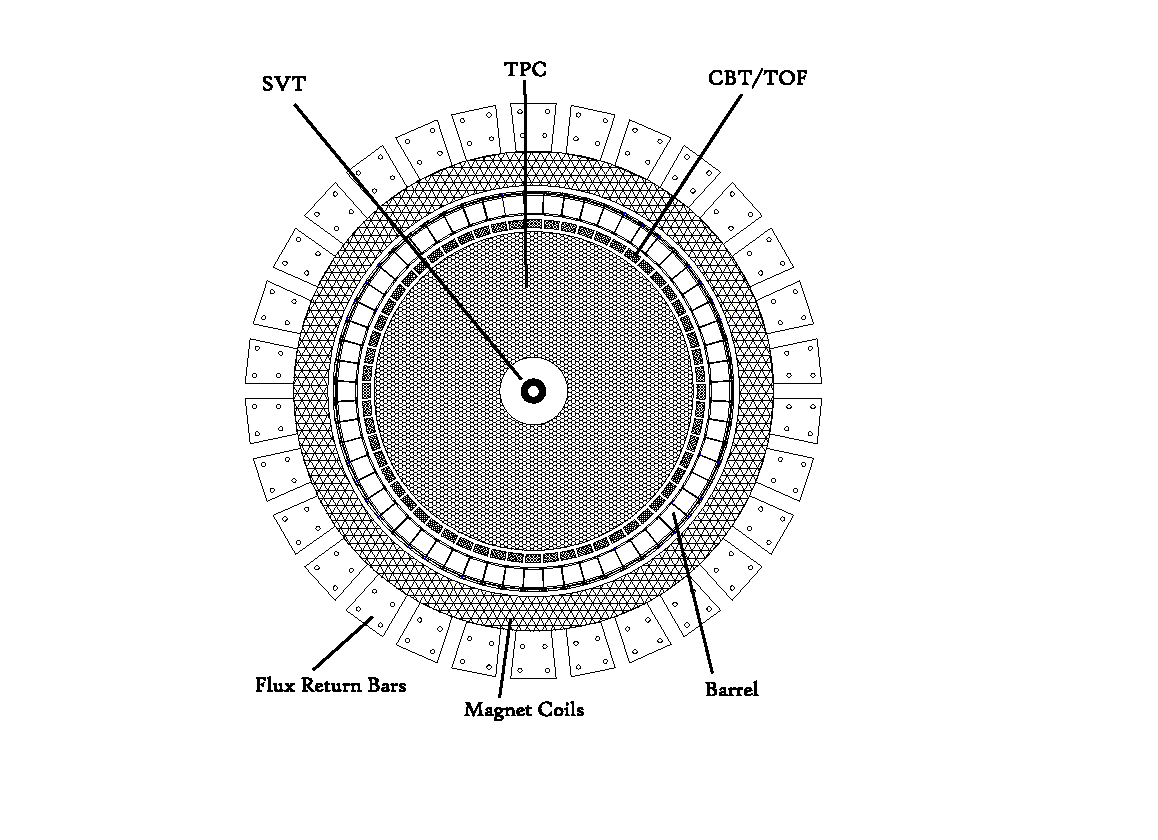
\includegraphics[scale=0.8]{ExperimentalAspect/BEMC_cs.eps}
    \subcaption{BEMC Cross Section view}
    \label{fig:bemcxsec}    
\end{subfigure}
\begin{subfigure}{0.8\textwidth}
\centering
    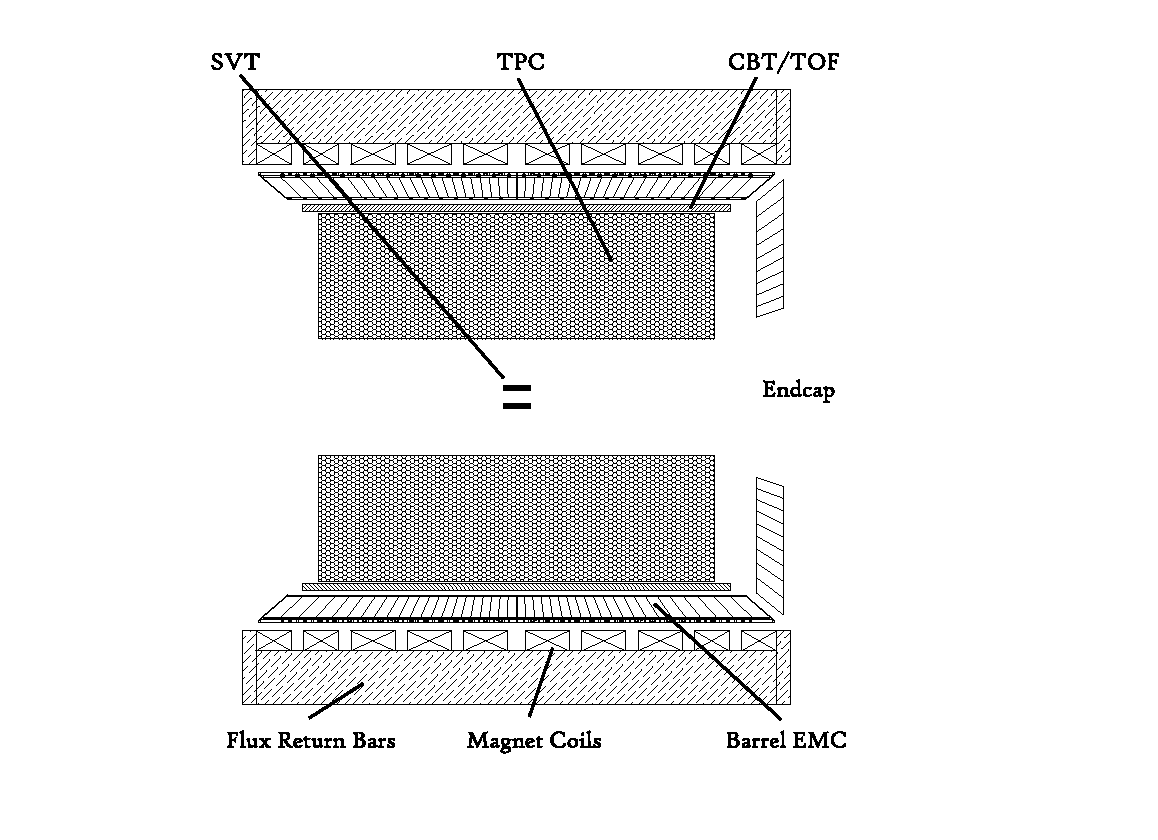
\includegraphics[scale=0.8]{ExperimentalAspect/BEMC_side.eps}
    \subcaption{BEMC Side view}
    \label{fig:bemcside}
 \end{subfigure}
 
\end{figure}
The BEMC design includes 120 calorimeter modules placed 60 in $\phi$ and 2 in $\eta$. Each module measures about 26 cm wide and 293 cm long with an active depth of 23.5 cm, each subtending 6\textdegree\  in $\Delta \phi$ and 1 unit in $\Delta\eta$. Each module is divided into 40 towers, 20 in $\eta$ and 2 in $\phi$, with each tower subtending 0.05$\times$0.05 in $\Delta\phi \times \Delta\eta$.  Thus, the BEMC comprises 4800 calorimeter towers spanning a full $2\pi$ coverage in azimuth. Each of the towers is constructed so that they point to the interaction diamond at the center. This projective nature of the tower in a module is shown in figure \ref{fig:bemcproj}.

\drawgraphics{1}{ExperimentalAspect/BEMC_sideprojective.eps}{Side view of the BEMC module.}{fig:bemcproj}

The core of the calorimeter consists of a stacked layer of 5 mm thick lead and 5 mm plastic scintillator alternately and a Shower Max Detector (SMD) situated roughly at five radiation lengths from the front of the stack. There are 21 active scintillating layers and 20 layers of lead absorber plates. The plastic scintillator, called ``megatile", consists of 40 optically isolated tiles. The mechanical structure of a calorimeter module with the compression components and the rail mounting system is shown in figure \ref{fig:bemcmoduleside}.
 
\subsection{Time of Flight (TOF)}
\label{subsec:tof}
The STAR Time of Flight (TOF) compliments the particle identification capability of the TPC by using the timing information in conjunction with the vertex position detector (VPD). TOF sits outside the TPC, wrapping all around and spanning the same coverage as the TPC. The TOF system is designed based on the multi-gap resistive plate chamber (MRPC), first developed by the CERN ALICE group \cite{Williams:2001mt}. The side view of the MRPC module for the STAR TOF system is shown in Figure \ref{fig:tofmodule}. The long edge of the module is shown at the top, whereas the bottom figure shows the short edge. The MRPC module consists of a series of  0.54 mm thick glass plates kept parallel by using 0.22 mm diameter nylon fishing line as a spacer. A mixture of 90\% C2H2F4, 5\% isobutane, and 5\% SF6 fills the gaps between the plates. The resistivity of these glass plates is of the order of $10^{13}$ \si{\ohm}/cm, thus being transparent to the electrical charges. These plates are electrically floating, and a strong electric field is generated in each sub-gap of gas with the electrodes applied on the outer surface of the outer plate. Since the glass plates and electrodes are charge transparent, the induced signal picked up by the copper readout pad is the sum of all the avalanche of charges induced in the gas gaps.  

The TOF system measures time intervals for a particle track using two detectors; one is the VPD (see section \ref{subsec:vpd} for details), which provides an event start time, and the TOF MRPC provide the stop time for reconstructed charged tracks that point back to the event vertex. This time interval, $\Delta t$, for reconstructed tracks, with the momentum, $p$, and total path length, $s$, allows us to calculate the inverse velocity, $1/\beta$, for each track as, 
\begin{equation}
    \frac{1}{\beta}  = \frac{c\Delta t}{s},
\end{equation}
where $c$ is the speed of light. With $1/\beta$ and $p$, the particle mass, $m$, can be calculated as,
\begin{equation}
    m = p \sqrt{1/\beta^2 -1}
\end{equation}

$\beta$, as calculated above using the TOF system timing information, versus particle momentum provides a basis for the TOF particle identification. 

In recent studies, it has been observed that for an event vertex with the z-vertex position difference identified by the TPC  ($V_{z,tpc}$) and VPD ($V_{z,vpd}$) greater 5 cm, the VPD timing information may be incorrect. 
A new method was developed called ``StartLessTOF", which addresses this issue by calculating the start time starting at the stop time and moving backward for a track without relying on the VPD timing. In the IFF asymmetry analysis, discussed in chapter \ref{chapter:iff}, the StartLessTOF method of PID is used, and more details will be discussed in the respective section.  

\drawgraphics{0.9}{./ExperimentalAspect/TOFmodule.jpg}{Side view of an MRPC module for the long (top) and short (bottom) sides.}{fig:tofmodule}

\subsection{Vertex Position Detector (VPD)}
\label{subsec:vpd}
There are two identical Vertex Position Detector (VPD) \cite{Llope:2014nva} assemblies, one at the east side and the other at the west side, located symmetrically surrounding the beam pipe at a distance of 5.7 m from the TPC center. Each VPD assembly consists of nineteen detectors, each composed of a lead (Pb) converter followed by a plastic scintillator read out by a photo-multiplier tube. The side view of this detector assembly is shown in figure \ref{fig:vpdside}. The front view of the VPD with all nineteen detectors assembled in two circles is shown in figure \ref{fig:vpdfront}.  

\drawgraphics{0.8}{./ExperimentalAspect/VPDfrontview.png}{VPD front view.}{fig:vpdfront}

\drawgraphics{0.8}{./ExperimentalAspect/VPDsideview.png}{VPD side view.}{fig:vpdside}

The VPD can provide timing information of an event, which is required for event triggering and for a fast detector as the event start time, for example, TOF. It measures the vertex $z-$position. It provides the timing information by measuring photon arrival time produced by the decay of $\pi^0$ in the very forward direction, close to the beam pipe.   

Besides serving as the primary detector input for the minimum bias trigger in A+A collisions, each VPD assembly measures up to nineteen times in each event, which is used to measure the location of the vertex along the beam direction, $Z_{vtx}$, given by,
\begin{equation}
    Z_{vtx} = c(T_{east} - T_{west})/2,
    \label{eq:vzvpd}
\end{equation}
where $T_{east}$ and $T_{west}$ are the times measured by the two VPD assemblies. Moreover, the start time used by the TOF for the particle identification, $T_{start}$ is given by, 
\begin{equation}
    T_{start} = (T_{east} + T_{west})/2 - L/c,
\end{equation}
where L is the distance of either assembly from the center of the STAR. The experimental resolution of the VPD timing, $T_{east}$ or $T_{west}$, depends on the number of channels used in the assembly $N$, which improves as $\delta T \propto 1/\sqrt{N}$, where $T$ is $T_{east} $ or $T_{west}$. Which follows the $Z_{vtx}$ resolution of equation \ref{eq:vzvpd} given by, 
\begin{equation}
    \delta Z_{vtx} =(c/2)\delta \Delta T = (c/\sqrt{2})\sigma_0 /\sqrt{N},
\end{equation}
where $\sigma_0$ is the time resolution of the single readout detector and $\delta \Delta T$ is the resolution of the time difference ($T_{east} - T_{west}$). Thus, the large number of readout channels allows averaging over more lit channels, improving the overall VPD performance.  


 

\chapter{\pip AZIMUTHAL CORRELATION ASYMMETRY}
\label{chapter:iff}
In this chapter, we will explore the precision measurement of the dihadron azimuthal correlation asymmetry \aut\ for the \pip\ in polarized proton-proton ($p^\uparrow p$) collisions based on the theoretical framework discussed in section \ref{sec:ifftheory}. This measurement is based on the STAR polarized $pp$ data from the Run 2015, which corresponds to the integrated luminosity, $L_{int}$, of $\sim $52 $pb^{-1}$, which can provide the most statistical precision in the asymmetry  in the valence quark region ($0.1<x<0.3$). I will discuss some of the asymmetry extraction methods, followed by a brief review of previous STAR measurements in the same framework. The rest of the chapter will provide the detail of the analysis. 

\section{\aut\ Extraction Methods}
In the STAR experiment, the asymmetry \aut\ can be extracted in $p^\uparrow p$ collisions by counting the number of dihadron pairs in different $\phi_{RS}$ bins for various beam polarization conditions (up and down). Two commonly employed methods for extracting \aut\ are discussed below.   
\subsection{Relative Luminosity Method}
The relative luminosity formula is given by

\begin{equation}
A_{UT}\ \sin \phi_{RS} = \frac{1}{P} \cdot \frac{N^\uparrow (\phi_{RS}) - r \cdot N^\downarrow (\phi_{RS})}{N^\uparrow (\phi_{RS}) + r \cdot N^\downarrow (\phi_{RS})},
\end{equation}

where $N^\uparrow (\downarrow)$ represents the number of dihadron pairs in each $\phi_{RS}$ bin when the beam is polarized up (down). The parameter $r$ corresponds to the ratio of the luminosities $L^\uparrow$ and $L^\downarrow$, while $P$ represents the absolute beam polarization.

Since the observed asymmetry is expected to be small, it is crucial to have precise measurements of the luminosities at different beam polarizations. However, at STAR, the uncertainty associated with the luminosity measurement is significant. This introduces a large systematic uncertainty in the obtained physics results. Considering the challenges posed by the large systematic uncertainty, the method relying on luminosity measurements is not adopted in this particular measurement. Alternatively, the cross-ratio method that doesn't involve any detector-related parameters is employed.

\subsection{Cross Ratio Method}
The cross-ratio method, which eliminates the need for detector-related quantities and reduces associated systematic uncertainties, is extensively discussed in reference \cite{Ohlsen:1973wf}. In the following, we outline the derivation of the cross-ratio formula for the spin-$\frac{1}{2}$ analyzing power in a symmetric detector system.

The cross section for a polarized spin-$\frac{1}{2}$ beam can be written as, 
\begin{equation}
    \label{eq:cr1}
    I(\theta, \phi) = I_0 (\theta) [1+p_y A_y(\theta)],
\end{equation}
where $\theta$ is the scattering angle, $I_0$ is the unpolarized cross section at an scattering angle $\theta$, $p_y$ is $y-$ component of the beam polarization, and $A_y(\theta)$ is the analyzing power. In terms of $p^\uparrow p$ to dihadron channel, the above equation can be expressed as, 
\begin{equation}
    \label{eq:cr2}
    I(\theta, \phi_{RS}) = I_{0,\phi_{RS}} (\theta) [1+P\ A_{UT}\ sin \phi_{RS} ], 
\end{equation}
where $P$ is the absolute polarization of the transversely polarized beam. 
Then the number of dihadrons recorded in particular $\phi_{RS}$ bin when the beam is polarized up $N^\uparrow_{\phi_{RS}}$ is given by, 
\begin{equation}
    N^\uparrow(\phi_{RS}) = L^\uparrow I_{0,\phi_{RS}}[1+A_{UT}\ P\ sin\phi_{RS}],
\end{equation}
where $L^\uparrow$ is the luminosity when the beam is polarized up.
In the same $\phi_{RS}$ bin, the dihadron counts when the polarization is flipped $N^\downarrow_{\phi_{RS}}$ is given by, 
\begin{equation}
    N^\downarrow(\phi_{RS})= L^\downarrow I_{0,\phi_{RS}}[1-A_{UT}\ P\ sin\phi_{RS}],
\end{equation}
where the negative sign is for the spin flipped.

It is expected that, by the rotational symmetry in a perfectly symmetric detector, the observed counts in a $\phi_{RS}$ bin when beam polarization is $\uparrow$ should be similar in the opposite $\phi_{RS}$ bin shifted by $\pi$, i.e., $\phi_{RS}+\pi$, when the beam is polarized $\downarrow$. So, the counts in the $\phi_{RS}+\pi$ bin when beam polarization up, $N^\uparrow(\phi_{RS+\pi})$, is given by, 
\begin{equation}
    N^\uparrow(\phi_{RS} +\pi)= L^\uparrow I_{0,\phi_{RS}+\pi}[1-A_{UT}\ P\ sin\phi_{RS}],
\end{equation}
where the negative sign is from $sin(\phi_{RS}+\pi) = - sin \phi_{RS}$. Again, the counts in the $\phi_{RS}+\pi$ bin when spin is flipped, $N^{\downarrow}(\phi_{RS}+\pi)$, is given by, 
\begin{equation}
    N^\downarrow(\phi_{RS} +\pi)= L^\downarrow I_{0,\phi_{RS}+\pi}[1+A_{UT}\ P\ sin\phi_{RS}],
\end{equation}
where the sign is positive because of an extra negative sign from the spin-flip. Now, forming a geometric mean of counts from equivalent bins as, 
\begin{equation}
\label{eq:l}
    \sqrt{N^\uparrow(\phi_{RS}) N^\downarrow(\phi_{RS}+\pi)} = \sqrt{L^\uparrow L^\downarrow I_{0,\phi_{RS}} I_{0,\phi_{RS}+\pi}}\ [1+A_{UT}\ P\ sin\phi_{RS}],
\end{equation}
and, 
\begin{equation}
\label{eq:r}
    \sqrt{N^\downarrow(\phi_{RS}) N^\uparrow(\phi_{RS}+\pi)} = \sqrt{L^\uparrow L^\downarrow I_{0,\phi_{RS}} I_{0,\phi_{RS}+\pi}}\ [1-A_{UT}\ P\ sin\phi_{RS}]
\end{equation}

Solving equations \ref{eq:l} and \ref{eq:r} for $A_{UT}sin\phi_{RS}$, we get, 
\begin{equation}
\label{eq:crossratio}
    A_{UT}\ sin\phi_{RS} = \frac{1}{P}\cdot \frac{\sqrt{N^\uparrow(\phi_{RS})N^\downarrow(\phi_{RS}+\pi)} -\sqrt{N^\downarrow(\phi_{RS})N^\uparrow(\phi_{RS}+\pi)}}{\sqrt{N^\uparrow(\phi_{RS})N^\downarrow(\phi_{RS}+\pi)} +\sqrt{N^\downarrow(\phi_{RS})N^\uparrow(\phi_{RS}+\pi)}}
\end{equation}

Equation \ref{eq:crossratio} is the cross-ratio formula, also called the ``geometric mean formula", which only involves the numbers without any  of the detector terms. This formula has a simple and elegant structure, which is why it has been widely used by STAR measurements, since the 2006 analysis-the first asymmetry analysis via dihadron channel in $p^\uparrow p$.

\section{STAR \aut\ : Proof-of-principle And Global Impact}

STAR reported the first measurement of \aut\  for \pip\  in $p^\uparrow p$ collisions at $\sqrt{s}=200$ GeV using Run 2006 data \cite{STAR:2015jkc}. This was followed by a measurement using Run 2011 data at $\sqrt{s}=500$ GeV \cite{STAR:2017wsi}. The 2006 dataset corresponds to an integrated luminosity of $L=1.8 \ \mathrm{pb}^{-1}$ and an average beam polarization of approximately 60\%, allowing for the exploration of the valence quark transversity in the range $0.15<x<0.30$. The 2011 data correspond to an integrated luminosity of 25 $\mathrm{pb}^{-1}$ with an average beam polarization of 53\% and covers a probing range in $x$ of about $0.05<x<0.2$.

\begin{figure}
    %\centering
    \begin{subfigure}{0.8\linewidth}    
    \centering
    \includegraphics[scale=0.4]{Results/PreviousSTARIFF/IFF_fig2_200.png}
    \subcaption{}
    \label{subfig:auteta200}
    \end{subfigure}
    %\hfill
    \begin{subfigure}{0.8\linewidth}    
    \centering
    \includegraphics[scale=0.4]{Results/PreviousSTARIFF/IFF_fig3_200.png}
    \subcaption{}
    \label{subfig:autmass200}
    \end{subfigure}
    %\captionsetup{justification=raggedright,singlelinecheck=false}
    \caption{\textbf{STAR $A_{UT}$ at $\sqrt{s}=200\ GeV -$} \textbf{(a)}  $A_{UT}$ as a function of \minv (upper panel) and corresponding partonic variables $x$ and $z$ (fraction energy of fragmenting quark carried by the \pip pair) (lower panel) from the simulation. \textbf{(b)} $A_{UT}$ as a function of \etap (upper panel) and $x$ and $z$ in the lower panel.} 
    \label{fig:aut200}
\end{figure}
Figure \ref{fig:aut200} shows the STAR \aut\ results at $\sqrt{s}=200$ GeV \cite{STAR:2015jkc}. Figure \ref{subfig:autmass200} depicts \aut\ as a function of the invariant mass (\minv) in two pseudorapidity bins, \etap $>0$ and \etap $<0$ in the top panel, whereas the bottom panel shows the partonic variables $x$ and $z$ (fractional energy of fragmenting quark carried by the \pip) from simulation in the same \minv\ bins. Figure \ref{subfig:auteta200} shows \aut\ as a function of \etap\ integrating over \minv\ and \ptp in the top panel and $x$ and $z$ in the bottom panel. The STAR \aut\ results at $\sqrt{s}=500$ GeV is shown in figure \ref{fig:aut500}. The signal differential in mass  in the forward \etap region plotted together with the STAR 2006. The theoretical prediction is shown in figure \ref{subfig:autmass500} and Figure \ref{subfig:auteta500} shows the \aut\ signal differential in \etap \ (top panel) and $x$ and $z$ in the corresponding \etap\ bins (bottom panel). 

The measured \aut\ signal exhibits significant magnitudes in the \etap$>0$ (forward) region, corresponding to the higher $x$ range where transversity is expected to be sizable. Conversely, the observed signal is small in the \etap$<0$ (backward) regions, which probe low $x$ values. This observation suggests a dependence of transversity on $x$. Additionally, the forward $A_{UT}$ signal exhibits a peak around the $\rho$-meson mass ($\sim 0.77$ GeV/$c^2$). This characteristic is anticipated due to the interference between pions originating from different production channels as is discussed in section \ref{sec:ifftheory}. Figure \ref{subfig:autmass500} compares the STAR 2006 and 2011 measurements with the theoretical calculations in \minv\ bins. The measured asymmetries and the resonance peak align well with the theoretical predictions. 

The STAR 2006 \aut\ data points obtained at $\sqrt{s}=200$ GeV have been incorporated into the global analysis for transversity extraction, alongside the SIDIS and $e^+e^-$ data \cite{Radici:2018iag}. Figure \ref{fig:h1} illustrates the behavior of $xh_1$ with and without the inclusion of the STAR data. Specifically, Fig. \ref{subfig:h1u} depicts the valence $u$-quark transversity ($xh_1^{u_v}$), while Fig. \ref{subfig:h1d} displays the valence $d$-quark transversity ($xh_1^{d_v}$) as functions of $x$. The dark band in Fig. \ref{subfig:h1u} and the light-hatched band in Fig. \ref{subfig:h1d} represent the inclusion of the STAR data, which is compared against the same result without the STAR data \cite{Radici:2015mwa}. Despite the statistical limitations, the impact of the STAR data is significant and results in notable improvements in constraining transversity in the valence quark region.


\begin{figure}
    \centering
    \begin{subfigure}{0.8\linewidth}    
    \centering
    \includegraphics[scale=0.4, trim=1.5cm 0.0cm 0.2cm 0.0cm]{Results/PreviousSTARIFF/AvsEtaPlot_v9.png}
    \subcaption{}
    \label{subfig:auteta500}
    \end{subfigure}
    \hspace{0.05em}
    \begin{subfigure}{0.8\linewidth}    
    \centering
    \includegraphics[scale=0.4, trim=1cm 0.0cm 0.5cm 0.0cm]{Results/PreviousSTARIFF/TheoryComparison_v5.png}
    \subcaption{}
    \label{subfig:autmass500}
    \end{subfigure}
    %\captionsetup{justification=raggedright,singlelinecheck=false}
    \caption{\textbf{STAR $A_{UT}$ at $\sqrt{s}=500\ GeV -$} \textbf{(a)} $A_{UT}$ as a function of \etap for $<p_T^{\pi^+\pi^-}> = 13 \ GeV/c$(top panel), and $x$ and $z$ in corresponding \etap bins (lower panel). \textbf{(b)} $A_{UT}$ as a function of \minv compared with the theory predictions from the SIDIS and $e^+e^-$ data  \cite{radici2016exploring} and STAR 2006 result.} 
    \label{fig:aut500}
\end{figure}

\begin{figure}
    %\centering
    \begin{subfigure}{0.8\linewidth}    
    \centering
    \includegraphics[scale=0.6]{Results/PreviousSTARIFF/fig1a_h1u.png}
    \subcaption{}
    \label{subfig:h1u}
    \end{subfigure}
    \hfill
    \begin{subfigure}{0.8\linewidth}    
    \centering
    \includegraphics[scale=0.6]{Results/PreviousSTARIFF/fig1b_h1d.png}
    \subcaption{}
    \label{subfig:h1d}
    \end{subfigure}
    %\captionsetup{justification=raggedright,singlelinecheck=false}
    \caption{ \textbf{Transversity $xh_1$ as a function of $x$ at $Q^2 = 2.4\ GeV^2$. The dark (blue) lines represent Soffer bounds. $-$} \textbf{(a)} Valence $u$-quark transversity. The dark band includes STAR $pp$, SIDIS, and $e^+e^-$, whereas the lighter band excludes the STAR data. \textbf{(b)} Valence $d$-quark transversity. The dark band only includes SIDIS and $e^+e^-$ data, and the lighter-hatched band is after including the STAR data. Significant improvement in the $xh_1$ because of the STAR data can be observed.} 
    \label{fig:h1}
\end{figure}

The measurement conducted using the Run 2015 dataset (this measurement) provides the most precise determination of \aut\ at $\sqrt{s}=200$ GeV. Consequently, this measurement will greatly enhance the precision in constraining transversity in the valence quark region.

\section{STAR Run 2015 IFF Analysis}

\subsection{Dataset and Quality Analysis}
To measure the IFF asymmetry, transversely polarized proton-proton collision data  from the STAR run 2015 at $\sqrt{s}=200$ GeV is utilized. The description of the data set is as follows:
\begin{itemize}
    \item Collision: proton-proton
    \item Center-of-mass energy ($\sqrt{s}$): 200 GeV 
    \item Beam polarization: transverse
    \item Production year: year2015
    \item Trigger Sets: production\_pp200trans\_2015
    \item Production tag: P16id
    \item Production library: SL16d
    \item Integrated luminosity ($L_{int}$): $\sim 52\ pb^{-1}$
\end{itemize}
The data included in this analysis consists of collision events that are triggered by dominant jet patch triggers. We have chosen to focus on events that were triggered by JP1 and JP2 (labeled as "JP"), which make up about 90\% of the total events. Specifically, events are selected with offline triggered IDs (JP1: 480404,480414) and (JP2: 480401,480411). It's worth noting that two different offline trigger IDs were used for the JP triggers because the trigger ID was changed after one-third of the data was collected during the data-taking process.

The data QA is performed at the event level, looking at the average of the quantities for every run. Runs with a run time of less than three minutes are excluded. In addition to the run time, the other primary criterion for a run  is to have JP-triggered events. Since this analysis is polarization sensitive, two fills reported with bad polarization patterns (fills 18749 and 18764 ) are excluded.


For QA purposes, the following event and track quality cuts are applied,
\begin{itemize}
    \item Z-Vertex ($V_z$): $|V_z|<60$ cm
    \item Vertex ranking ($V_{z,rank}$): $V_{z,rank}>1e6$
    \item Track pseudorapidity ($\eta_{tr}$): $|\eta_{tr}|<1$
    \item Track transverse momentum ($p_T$): $p_T > 1.5$
    \item Track distance of closest approach ($dca$): $dca < 1$
            \[
            dca = \begin{cases}
            2\ cm & \text{if } p_T < 0.5\ \text{GeV}, \\
            2.5\ cm - p_T (1\ cm /GeV) & \text{if } 0.5< p_T< 1.5\ GeV, \\
            1\ cm & \text{if } p_T \geq 1.5 \ GeV
            \end{cases}
            \]
    
    \item Number of fit points (nHitsFit): $nHitsFit>25$
    \item  Fit points ratio (nHitsFit/nHitsFitPoss): $nHitsFit/nHitsFitPoss>0.51$
    \item Pion selection: $-1<n\sigma_\pi<2$
\end{itemize}

\drawgraphics{0.8}{Results/IFF2015/EventQA/TrackpTEtaPhi300.png}{ Average track $\eta$, $\phi$, and $p_T$ per run.}{fig:qa}

All the primary tracks originating from primary vertices are used. The cuts on $V_z$ and $V_{z,rank}$ remove pileup vertices. Tracks with higher TPC hits have higher precision than those with fewer fit points. The track cut on $\eta$ limits the track within the TPC acceptance in the central region. The fit points ratio cut prevents double counting tracks with different segments reconstructed as independent tracks. The $dca$ cut removes tracks from secondary decays. This set of selection cuts was specifically used for the QA analysis; the physics analysis cuts will be discussed in the respective section. 

The average event and track parameters per run, such as $v_z$, $\eta$, $\phi$, $p_T$, etc.,  are plotted as a function of the run index. Ideally, the average value per run throughout the run period should be consistent. However, several environmental and experimental conditions affect the data-taking process resulting in event records that may not be useful for the physics analysis. Any run with an average value outside $3\sigma$ from the mean is excluded.

Figure \ref{fig:qa} shows the average of track $p_T$, $\eta$, and $\phi$ for JP1 and JP2 triggers plotted as a function of the run index after QA for the first 300 runs. The average values feature the fill dependence, where each band corresponds to one fill. After QA, 749 good physics runs are found to be good for the physics analysis. A list of good runs can be found in the appendix \ref{appsec:runlist2015}.

\subsection{Simulation and Comparison with Data}
This analysis requires a Monte Carlo simulation sample to estimate systematic uncertainty due to the event triggering. Simulated events are generated using PYTHIA 6.4.28 \cite{pythia} with the Perugia 2012 tune \cite{Skands:2010ak}. In Perugia 2012, the parameter PARP(90), which controls the energy dependence of the underlying event processes low$-p_T$ cut-off, is adjusted from 0.24 to 0.213 to match STAR-specific measurements of the $\pi^\pm$ cross sections in 200 GeV $pp$ collisions \cite{STAR:2003oii, STAR:2011iap}. This modification has provided a good description of jet and underlying event properties in $pp$ collisions for both 200 \cite{STAR:2019cie, STAR:2020ejj, STAR:2021lvw} and 510 \cite{STAR:2019yqm} GeV energies. The simulated events are then processed through full detector simulations that match the detector configurations in 2015 runs implemented in GEANT 3 \cite{geant}. The GEANT 3 simulation fully replicates the STAR 2012 detector configuration. However, for the run 2015, additional material from the Heavy Flavor Tracker (HFT) \cite{Bouchet:2009id} in the region $|z| \lesssim 30$ cm is included. To account for this extra material effect, the GEANT simulation is conducted using the 2012 detector configuration but digitized with the routines that describe the detector readout in 2015\cite{STAR:2022hqg}. Event pileup and beam background effects are incorporated by embedding simulated events into the zero-bias events collected during 2015 runs. The zero-bias events are triggered on the bunch crossings at the clock trigger, which is uncorrelated with the collision. In addition, the  online trigger algorithm is implemented in the embedding sample, which allows trigger selection in the embedding sample.

The simulation software records hard scattered partons, final state particles from the fragmentation and hadronization of partons, and the detector's response to the final state particles. The final state particles are referred to as ``particle level", while their response to the detector is called  ``detector level". The detector responses are recorded in the same format as those generated in real data events. 

The detector level quantities from the embedding must have a good description of the real data to apply the embedding-driven measurement directly to the measurement from the data. The data and embedding are compared separately for all relevant physics quantities for the JP1 and JP2 triggers. 
As the embedding sample is produced with the increasing partonic $p_T$ ($\hat{p_T}$) to ensure the comparable embedding statistics to the triggered statistics in the data, we need to combine all the $\hat{p_T}$ bins. To combine the $\hat{p_T}$ bins, a weight proportional to the number of events generated in the particular $\hat{p_T}$ bin  is used. The weight is simply an inverse of the luminosity for each $\hat{p_T}$, $\mathcal{L}_i = N_i\hat{\sigma}_i$, where $N_i$ is the total generated events in the $\hat{p_T}$ bin $i$ and $\hat{\sigma}$ is the corresponding partonic cross section. Furthermore, the luminosity is normalized by the luminosity of the highest $\hat{p_T}$ bin, such that the weight is one for the highest bin. The assurance of the reliable recombination of $\hat{p_T}$ bins is provided by the full $\hat{p_T}$ spectrum; it is expected to be a smooth distribution overall range of the $\hat{p_T}$. Figure \ref{fig:partonicpt} shows the weighted $\hat{p_T}$ combining all the partonic bins. The smoothness of the curve suggests that the weighting scheme is working perfectly. 
 
\begin{figure}
    \centering
    \includegraphics{Results/IFF2015/DatEmbed/partonicpt_wt.png}
    \caption{Weighted partonic $p_T$ distribution.}
    \label{fig:partonicpt}
\end{figure}

Figure \ref{fig:piptpos} and \ref{fig:piptneg} shows the $p_T^{\pi^+}$ and $p_T^{\pi^-}$  comparison between the data and embedding for JP1 (left panel) and JP2 (right panel), respectively. A good data description by embedding over a wide $p_T$ range can be seen. The full comparison plots for the event and track-level quantities are shown  in appendix \ref{app:run15dataembed}. In the embedding, JP1 and JP2 triggers are combined using the prescale values from the data. The prescale value of 5.887 for the  JP1 trigger is used while combining distribution with the JP2, which has a prescale value of one. 

\begin{figure}[H]
    \centering
    \begin{subfigure}{0.45\linewidth}
        \includegraphics[scale=0.35]{Results/IFF2015/DatEmbed/pTPJP1.png}
    \end{subfigure}
    \hspace{0.2em}
    \begin{subfigure}{0.45\linewidth}
        \includegraphics[scale=0.35]{Results/IFF2015/DatEmbed/pTPJP2.png}
    \end{subfigure}
    \caption{$p_T^{\pi^+}$  for JP1 and JP2.}
    \label{fig:piptpos}
\end{figure}

\begin{figure}[H]
    \centering
    \begin{subfigure}{0.45\linewidth}
        \includegraphics[scale=0.35]{Results/IFF2015/DatEmbed/pTNJP1.png}
    \end{subfigure}
    \hspace{0.2em}
    \begin{subfigure}{0.45\linewidth}
        \includegraphics[scale=0.35]{Results/IFF2015/DatEmbed/pTNJP2.png}
    \end{subfigure}
    \caption{$p_T^{\pi^-}$  for JP1 and JP2.}
    \label{fig:piptneg}
\end{figure}

\begin{figure}[H]
    \centering
    \begin{subfigure}{0.45\linewidth}
        \includegraphics[scale=0.35]{Results/IFF2015/DatEmbed/ptPairJP1.png}
    \end{subfigure}
    \hspace{0.2em}
    \begin{subfigure}{0.45\linewidth}
        \includegraphics[scale=0.35]{Results/IFF2015/DatEmbed/ptPairJP2.png}
    \end{subfigure}
    \caption{\ptp\  for JP1 and JP2.}
    \label{fig:piptneg} 
\end{figure}

\begin{figure}[H]
    \centering
    \begin{subfigure}{0.45\linewidth}
        \includegraphics[scale=0.35]{Results/IFF2015/DatEmbed/MinvJP1.png}
    \end{subfigure}
    \hspace{0.2em}
    \begin{subfigure}{0.45\linewidth}
        \includegraphics[scale=0.35]{Results/IFF2015/DatEmbed/MinvJP2.png}
    \end{subfigure}
    \caption{\minv\ for JP1 and JP2.}
    \label{fig:piptneg}
\end{figure}

\subsection{Events and Track Selection Cuts}
\label{subsec:finalcuts}

High-quality tracks associated with the event vertices within 60 cm along the beam direction from the nominal TPC center are used in this analysis. Each event should be JP-triggered and must have at least two quality tracks. Each track must have transverse momentum $p_T > 1.5 $ GeV/c and the distance of closest approach \emph{dca}$< 1$ cm from the event vertex. Charged pions are identified by measuring their ionization energy loss, $dE/dx$. Pions are selected by requiring a cut on the standard deviations of measured $dE/dx$ from the expected pion energy loss,  $-1< n\sigma_{\pi}< 2$, where $n\sigma_\pi$ is defined as, 
\begin{equation}
 n\sigma_\pi = \frac{1}{\sigma_{exp}} \mathrm{ln}(\frac{dE/dx_{obs}}{dE/dx_{\pi, calc}}) ,   
\end{equation}
where $dE/dx_{obs}$ is the observed value for the particle track, $dE/dx_{\pi, calc}$ is the expected mean $dE/dx$ for pions of the given momentum, and $\sigma_{exp}$ is the $dE/dx$ resolution of the TPC. 

\input{Results/IFF2015/Preliminary/table_selectioncuts}

\textbf{Terminology definitions:}
\begin{itemize}
	\item{Fit ratio = nHitsFit/nHitsFitPossible.}
        \item $\eta = - \mathrm{ln\ tan}(\frac{\theta}{2})$, where $\theta$ is the angle between the particle momentum and the positive direction of the beam axis.  
	\item{cone($\pi^+\pi^-$): Opening angle between $\pi^+$ and $\pi^-$  in $\eta - \phi$ space\\(cone$=\sqrt{(\eta^{\pi^+}-\eta^{\pi^-})^2 +(\phi^{\pi^+}-\phi^{\pi^-})^2}$).} 
    \item{$M_{inv}^{\pi^+\pi^-}$: Invariant mass of $\pi^+\pi^-$ pair($=\sqrt{2M_{\pi}^2 +2(E^{\pi^+}E^{\pi^-}-\vec{p}^{\pi^+}\cdot \vec{p}^{\pi^-})}$ ).}
	\item{$p_{T}^{\pi^+\pi^-}$: Transverse momentum of $\pi^+\pi^-$ pair relative to the beam direction ($=\sqrt{p_x^{{\pi^+\pi^-}^2}+p_y^{{\pi^+\pi^-}^2} }$ ).}
	\item{$\eta^{\pi^+\pi^-}$: Pseudorapidity of $\pi^+\pi^-$($=\arcsin(\frac{p_z^{\pi^+\pi^-}}{p_T^{\pi^+\pi^-}})$ ).}
\end{itemize}




\subsection{\pip\ Pair Reconstruction and Binning}

The \pip\ pairs are formed by selecting oppositely charged pion tracks and associated azimuthal angles and kinematics are constructed following geometry in the figure \ref{fig:angles}. All possible combinations of opposite pairs are formed for each event, without repetition (for example, \pip\ and $\pi^-\pi^+$ pair are the same, which are avoided!). The $\pi^+$ and $\pi^-$ tracks should be close enough in $\eta-\phi$ space (cone $\equiv \sqrt{(\eta^{\pi^+}-\eta^{\pi^-})^2+(\phi^{\pi^+}-\phi^{\pi^-})^2} < 0.7$). The cone cut ensures that the \pip\ is within the jet (note that jet reconstruction is not required, and the cone cut is applied to ensure the pair falls within the jet!). The pair kinematic variables are constructed with the formula listed in the section \ref{subsec:finalcuts}. The \pip\  pair invariant mass is denoted by \minv, the transverse momentum relative to the beam direction is denoted by \ptp\, and pseudorapidity is denoted by \etap, which are important pair level quantities in which asymmetry will be measured. Figure \ref{fig:pairkin} displays the reconstructed pair kinematic distributions.
\begin{figure}
    \centering
    \begin{subfigure}{0.45\linewidth}
        \includegraphics[scale=0.3]{Results/IFF2015/PairDist/cone.png}
        \subcaption{cone}
        \label{subfig:cone}
    \end{subfigure}
    \hfill
    \begin{subfigure}{0.45\linewidth}
        \includegraphics[scale=0.3]{Results/IFF2015/PairDist/mass.png}
        \subcaption{\minv}
        \label{subfig:mass}
    \end{subfigure}
    \hfill
    \begin{subfigure}{0.45\linewidth}
        \includegraphics[scale=0.3]{Results/IFF2015/PairDist/pt.png}
        \subcaption{\ptp}
        \label{subfig:pt}
    \end{subfigure}
    \hfill
    \begin{subfigure}{0.45\linewidth}
        \includegraphics[scale=0.3]{Results/IFF2015/PairDist/eta.png}
        \subcaption{\etap}
        \label{subfig:eta}
    \end{subfigure}
    \caption{\pip Kinematic distributions.}
    \label{fig:pairkin}
\end{figure}

\begin{figure}
    \centering
    \begin{subfigure}{0.45\linewidth}
        \includegraphics[scale=0.3]{Results/IFF2015/PairDist/phisBlue.png}
        \subcaption{$\phi_{S}$ Blue }
        \label{subfig:phisB}
    \end{subfigure}
    \hfill
    \begin{subfigure}{0.45\linewidth}
        \includegraphics[scale=0.3]{Results/IFF2015/PairDist/phisYellow.png}
        \subcaption{$\phi_{S}$ Yellow }
        \label{subfig:phisY}
    \end{subfigure}
    \caption{$\phi_{S}$ distributions for blue and yellow beam.}
    \label{fig:phis}
\end{figure}
    
 \begin{figure} 
    \centering
    \begin{subfigure}{0.45\linewidth}
        \includegraphics[scale=0.3]{Results/IFF2015/PairDist/phirBlue.png}
        \subcaption{$\phi_{R}$ Blue }
        \label{subfig:phirB}
    \end{subfigure}
    \hfill
    \begin{subfigure}{0.45\linewidth}
        \includegraphics[scale=0.3]{Results/IFF2015/PairDist/phirYellow.png}
        \subcaption{$\phi_{R}$ Yellow }
        \label{subfig:phirY}
    \end{subfigure}
    \caption{$\phi_R$ distributions for blue and yellow beam.}
    \label{fig:phir}
\end{figure}

The STAR coordinate system is followed for the reconstruction of the azimuthal angles. The blue beam direction is along the $+z$, and the yellow beam follows the $-z$ axis. For both beams, for a pair reconstruction, the polarization direction is fixed along the $+y$ axis as default. The $+x$ can be determined using the right-hand rule. The blue and yellow beam geometry differs in the $\eta-$ direction; the blue beam points from $-\eta$ to $+\eta$, whereas the yellow follows the opposite direction. To fix this kinematic difference, the sign of the $\eta$ of \pip\ events for the yellow beam is flipped, i.e., \etap (-\etap) $\rightarrow$ -\etap(\etap). The definition of azimuthal angle $\phi_{RS}(=\phi_{s}-\phi_{R})$ is illustrated in figure \ref{fig:pairkin}, which are constructed using equations \ref{eq:cosang} and \ref{eq:sinang}, where $\phi_{s}$ is an angle between the polarization vector, $\vec{s}_a$, and the scattering plane, formed by the beam momentum vector, $\vec{p}_{beam}$, and the \dipion\ momentum sum vector, $\vec{p}_h(=\vec{p}_{h,1}+ \vec{p}_{h,2})$. $\phi_{R}$ is an angle between the scattering plane and the \dipion\ plane, formed by two $\pi$'s momenta, $\vec{p}_{h,1}$, and $\vec{p}_{h,2}$. $\vec{R}(=\frac{1}{2}(\vec{p}_{h,1}-\vec{p}_{h,2}))$ is the relative momentum vector of the \dipion\ system. Here, $\vec{p}_{h,1}$ is reserved for $\pi^+$ and $\vec{p}_{h,2}$ for $\pi^-$. This charge ordering is important; otherwise, the direction of $\vec{R}$ is randomized, resulting in a diluted asymmetry (see appendix \ref{app:randomaut}).


\begin{figure}    
    \centering
    \begin{subfigure}{0.45\linewidth}
        \includegraphics[scale=0.3]{Results/IFF2015/PairDist/phirsBlue.png}
        \subcaption{$\phi_{RS}$ Blue}
        \label{subfig:phirsB}
    \end{subfigure}
    \hfill
    \begin{subfigure}{0.45\linewidth}
        \includegraphics[scale=0.3]{Results/IFF2015/PairDist/phirsYellow.png}
        \subcaption{$\phi_{RS}$ Yellow}
        \label{subfig:phirsY}
    \end{subfigure}
    \caption{$\phi_{RS} (= (\phi_{S} - \phi_{R})$ distributions for blue and yellow beam.}
    \label{fig:phirs}
\end{figure}


The \pip\ yields are sorted based on the beam polarization direction ($\uparrow/\downarrow$). The STAR 2015 data has both beams polarized in the transverse direction, and, advantageously, both beams can be treated separately for asymmetry measurement. Moreover, the spin patterns during the fill are set to fixed order, such that if we integrate the polarization states, the net polarization will turn out to be zero. This feature of the spin patterns of polarized beams at STAR makes it possible to perform physics analysis that uses unpolarized beams, such as the unpolarized cross-section measurement as discussed in the chapter \ref{chapter:xsec}. 

For the asymmetry measurement, yellow and blue beams are analyzed independently; while using yellow, the blue beam is treated as unpolarized, integrating all the spin states.  The decimal equivalent of the 8-bit spin pattern, listed below, is used to tag a beam polarization state (see appendix \ref{app:spinpattern}):
\begin{itemize}
    \item Blue $\uparrow$, Yellow $\uparrow$ $\equiv$ 51 (8-bit = 0011 0011)
    \item Blue $\downarrow$, Yellow $\downarrow$ $\equiv$ 85 (8-bit = 0101 0101)
    \item Blue $\uparrow$, Yellow $\downarrow$ $\equiv$ 53 (8-bit = 0011 0101)
    \item Blue $\downarrow$, Yellow $\uparrow$ $\equiv$ 83 (8-bit = 0101 0011)
\end{itemize}
This immediately follows that the \dipion yields from the blue $\uparrow$, $N^\uparrow_B$, is given by the spin states 51 and 53 and that from blue $\downarrow$ is given by 83 and 85. Similarly, the yellow $\uparrow$ yields are given by spin states 51 and 83, whereas the yellow $\downarrow$ yields are given by 53 and 85. These numbers tag yields from specific spin states at the analysis level. 

The \aut\ should be kept differential in as many as kinematic variables, which otherwise likely gets diluted \cite{Jaffe:1997}. In this analysis, \aut\ will be measured differentiated in \minv, \ptp, and \etap\ . The \etap\ is a surrogate of the partonic variable $x$, where, in the STAR coordinate system, \etap $>0 (<0)$ is the high(low)$-x$ region. Using a large data sample, each pair kinematics is divided into nine bins of varying width such that each bin contains roughly the same number of the \pip\ yields.

For the extraction of the amplitude of the sine modulation, each kinematic bin is further divided into 16 $\phi_{RS}$ bins, and  the \pip\ yields are counted in each $\phi_{RS}$ bin for each spin state. For example, $N^\uparrow (\phi_{RS})$ represents the yields in the $\phi_{RS}$ bin when the beam is polarized $\uparrow$. The measurement is performed for both polarized beams separately, and the final result is the weighted average of both. 

\subsection{Polarization Correction}
The beam polarization is recorded at the beginning of the fill and followed by subsequent measurements during the beam fill. Because of the depolarization as discussed in section \ref{subsec:snakes}, the beam polarization decay linearly. The slope of the linear polarization decay ($\frac{dP}{dt}$) is provided for each beam fill along with the initial polarization ($P_0$) at the beginning of the fill ($t_0$). At any time, $t$, the polarization value is given by, 
\begin{equation}
    P(t) = P_0 + \frac{dP}{dt} (t-t_0)
    \label{eq:pozdecay}
\end{equation}
\drawgraphics{0.8}{Results/IFF2015/PolzDist/polzDist.png}{Event-by-event polarization corrected values for blue and yellow beams.}{fig:avgpolz}

\drawgraphics{0.8}{Results/IFF2015/PolzDist/polzVsrunindex.png}{Event-by-event polarization corrected values vs run index for blue and yellow beams.}{fig:polzvsrun}

For every event, the actual polarization value is calculated using the equation above at the event time. The corrected polarization values for all events are filled in a histogram for every run for the blue and yellow beams, separately. Figure \ref{fig:avgpolz} shows the event-by-event corrected polarization distribution for a total data sample for blue and yellow beams, and corrected polarization as a function of the run index is shown in figure \ref{fig:polzvsrun}. From figure \ref{fig:avgpolz}, the corrected polarization are found to be, 
    \begin{itemize}
        \item $P_B$ = 57.11\% $\pm$ 3.75\% for the blue beam.
        \item $P_Y$ = 58.16\% $\pm$ 3.80\% for the yellow beam.
    \end{itemize}
The $P_B$ and $P_Y$ values and associated errors are used in the asymmetry calculation. The 3\%  systematic uncertainty from the beam polarization measurement is not included in the asymmetry extraction, which will be mentioned separately with the result.      

\subsection{\aut\ Extraction in $p^\uparrow p$}
Since the \pip\ azimuthal correlation asymmetry arises due to the convolution of $h_1(x)$ and $H_1^{\sphericalangle,\pi^+\pi^-}(z, M^2)$, it inherit the dependence on the partonic variable $x$ from $h_1(x)$ and the final state variables $z$ and $M$, from $H_1^{\sphericalangle, \pi^+\pi^-}(z,M^2)$. So, \aut\ is extracted in \minv\ , \ptp\ , $x$, and $z$ bins. Moreover, the asymmetry is extracted as a function of \minv\ in different \ptp\ bins and vice versa, which provides further granularity in the kinematics for the global extraction of transversity. 
\begin{figure}
    \centering
    \begin{subfigure}{0.6\linewidth}
        \includegraphics[scale=0.5]{Results/IFF2015/sinefit_blue.jpg}
        \subcaption{}
        \label{subfig:sineblue}
    \end{subfigure}
    \begin{subfigure}{0.6\linewidth}
        \includegraphics[scale=0.5]{Results/IFF2015/sinefit_yellow.jpg}
        \subcaption{}
        \label{subfig:sineyellow}
    \end{subfigure}
    \caption{``sine" modulation and fits for (a) Blue (b) Yellow beams in $\eta>0$ in the \ptp bin ([6.4 - 15) GeV/$c$)  and \mpair bin ([0.77, 0.88) GeV/$c^2$, where the asymmetry signal is largest.}
    \label{fig:sinefit}
s\end{figure}
\drawgraphics{0.8}{Results/IFF2015/mbin_chi2ndfAll.png}{$\chi^2$/ndf of the ``sine" fit in all kinematic bins. The quality of the ``sine" fit is monitored by the $\chi^2$/ndf ratio.}{fig:chi2ndf}

The cross ratio formula, given by equation \ref{eq:crossratio}, is used for the \aut\ extraction. The right side of the equation \ref{eq:crossratio} is calculated for the 8 - $\phi_{RS}$ bins in the range [$-\pi$, 0]. This is possible by dividing the whole $\phi_{RS}$ range into 16 bins of equal width  and counting yields in each bin when the beam is polarized up or down. Then these eight data points are fitted with the ``sine" function, allowing the amplitude to float freely. The amplitude of the fit and corresponding error is the \aut\ signal and associated statistical uncertainty in the particular kinematic bin. An example of the fit is shown in figure \ref{fig:sinefit} for the blue (\ref{subfig:sineblue}) and yellow (\ref{subfig:sineyellow}) beam in the same kinematic bin (\ptp[6.4, 15)(GeV/$c$) and \minv[0.8823, 1.031)GeV/$c^2$, \etap $>0$), where the asymmetry signal is largest. The central values are the numerical value from the right side of equation \ref{eq:crossratio} calculated using yields in 8-$\phi_{RS}$ bins, and the error bars are the statistical uncertainty calculated by the error propagation method. The functionality of the fit has a very good description, as indicated by the $\chi^2/ndf$ of the fit. Figure \ref{fig:chi2ndf} shows the $\chi^2/ndf$ distribution from the ``sine" fit for blue and yellow beam asymmetry in forward and backward pseudorapidity regions associated with the results shown in figure \ref{autM}. The same level of fit quality is observed in all kinematic bins.    
 
\subsection{Systematic Uncertainties}
\subsubsection{Pion Contamination Fraction}
 This measurement uses \pip\ pair for asymmetry measurement; however, any of the hadron pairs, such as \pip, $K^+K^-$, or $p\bar{p}$, can be used to achieve the same physics motivation. Different QCD mechanisms may be involved with the different hadron species resulting in different asymmetry signals. Thus, knowing the hadron purity in the kinematic bin where the asymmetry is measured is important. The STAR TPC measures the charged particle ionization loss, $dE/dx$, with which we can identify charged  particle species based on the track momentum and charge sign with the direction of curvature in the uniform magnetic field. The TPC, however, can identify particles of momentum $p < 1$ GeV/c with better precision, and the TPC capability degrades for the higher momentum particles. The STAR timing detector, TOF, compliments the TPC PID providing better resolution up to $p < 1.6 $ GeV/c; however, this measurement uses only the TPC information for the particle fraction calculation at the preliminary level, which is discussed in this section.
    \drawgraphics{0.8}{Results/IFF2015/Bichsel_I70.png}{Distribution of $log_{10}(dE/dx)$ as a function of $log_{10}(p)$ for pion, kaon, electron, proton, and their antiparticles. The units of $dE/dx$ and $p$ are KeV/cm and GeV/c, respectively. The color band represents the $\pm 1\sigma$ band of the $dE/dx$ resolution. I70 means Bichsel's prediction for 30\% truncated $dE/dx$ mean \cite{Shao:2005iu}.}{fig:pidbichsel}

Figure \ref{fig:pidbichsel} shows the $dE/dx$ as a function of particle track momentum in the logarithmic scale measured by TPC, together with Bichsel's prediction \cite{Shao:2005iu}. Each band represents the charged particle species. At the lower momentum region of $p<1$ GeV/c, $dE/dx$ for pions, kaons, protons, and electrons are separated. This allows the charge particle identification to higher precision in the lower momentum region. In the region $1 \leq p < 1.3$ GeV/c, the crossover of the $dE/dx$ bands takes place, which makes it difficult for particle identification in this region. However, beyond $p >1.3$ GeV/c, the relativistic rise of $dE/dx$ and lower electron and kaon yields, there is about 15\% difference in the $dE/dx$ between the pions and kaons, and that is even higher for the protons. So it is possible to identify pions from kaons and protons in the higher momentum region from the TPC alone; however, it is hard to identify kaons and protons as the  $dE/dx$ bands almost overlap. Since this analysis uses the pion tracks of $p_T\geq 1.5$ GeV/$c$, it skips the $dE/dx$ crossover region. The relativistic rise effect allows us to isolate the pions from the proton and kaon in this region; electrons are very few and well separated from pions. A standard approach adopted for calculating a fraction of other particle species ($p's, K's, e's$) that sneaks into the pion region using the $n\sigma_\pi$ distribution.

\drawgraphics{0.8}{Results/IFF2015/PrelimPID/nsigmapion_pt0bin.png}{n$\sigma_\pi^+$ distribution in the lowest \ptp\ bin (2.8 - 3.71 GeV/$c$) in \etap $>0$.}{fig:pionnsigma}

Figure \ref{fig:pionnsigma} shows the $n\sigma_\pi$ distribution for positive charge tracks in the lowest \ptp\ bin in \etap$>0$ region. The distribution has a prominent pion peak centered around zero. The proton and kaon appear on the left (p+k region), and the electron appears on the right of the pion peak. The selected pion region falls between the two vertical lines, which is selected with the cut in $n\sigma_\pi (-1<n\sigma_{\pi}<2)$. As the p+k falls very close to the pion, the major source of background in the pion signal region would be from the protons and kaons. The electron has a  distinct peak further away from the pion, which is easy to identify, and has a nominal presence in the pion signal region. Some tracks that appear on the far right, labeled ``Pile up", do not contribute to the pion signal region, so they are ignored.

A multi-gaussian fit method estimates other particle contributions in the pion signal region. First, we need to know the peak position of each particle species in the $n\sigma_\pi$ distribution to construct a multi-gaussian fit that describes the whole distribution. This can be done by constructing a two-dimensional (2D) distribution of $n\sigma_\pi$ along the $x-$axis and $n\sigma_{p, K, e}$ along the $y-$axis. A sample 2D plots of $n\sigma_p$ vs $n\sigma_{\pi^+}$ in five \ptp\ bins in the \etap$>0$ is shown in figure \ref{fig:pid2dfit}. A third-order polynomial fit (pol3) on the profile of the 2D histogram, which gives the average of $y-$values for each of the $x-$bin, allows finding the peak position along the $y-$axis corresponding to the pion mean position at zero along $x-$axis. In figure \ref{fig:pid2dfit}, the proton's peak position is reported in each of the \ptp\ bins. The same approach identifies peak positions for kaons and electrons, with reference to the pion peak at zero. 
    \drawgraphics{0.8}{Results/IFF2015/PrelimPID/cnSigmaPionVsProtonPosGt_pTbin.pdf}{ Track $n\sigma_\pi^+$ vs $n\sigma_p$  in five invariant mass bins.}{fig:pid2dfit}
    
    \drawgraphics{0.8}{Results/IFF2015/PrelimPID/pionFit_ptBinPosGt.pdf}{ Track $n\sigma_\pi^+$ multi-gaussian fit  in five invariant mass bins.}{fig:pidgausfit}
   
    \drawgraphics{0.7}{Results/IFF2015/PrelimPID/purity_pTbin.pdf}{ Particle fractions at the track level in the bins corresponding to the figure \ref{fig:pidgausfit}}{fig:trackpidpt}
    
    \drawgraphics{0.7}{Results/IFF2015/PrelimPID/purity_Mbin.pdf}{ Particle fractions at the track level in \minv bins.}{fig:trackpidmass}
    
    \drawgraphics{0.7}{Results/IFF2015/PrelimPID/purity_Etabin.pdf}{ Particle fractions at the track level in \etap bins.}{fig:trackpideta}

    
    \begin{figure}
        \centering
        \begin{subfigure}{0.45\linewidth}
        \centering
        \includegraphics[scale=0.4]{Results/IFF2015/PrelimPID/pairpurity_MBin.pdf}
        \captionsetup{justification=raggedright,singlelinecheck=false}
        \subcaption{\raggedright \pip\ fraction in \minv\ bins.}
        \label{subfig:purity_mbin}
        \end{subfigure}
        \hspace{0.2em} 
        \begin{subfigure}{0.45\linewidth}
        \centering
        \includegraphics[scale=0.4]{Results/IFF2015/PrelimPID/pairpurity_PtBin.pdf}
        \subcaption{\pip\ fraction in \ptp\ bins.}
        \label{subfig:purity_ptbin}
        \end{subfigure}
        \hfill
        \begin{subfigure}{0.45\linewidth}
        \centering
        \includegraphics[scale=0.4]{Results/IFF2015/PrelimPID/pairpurity_EtaBin.pdf}
        \subcaption{\pip\ fraction in \etap\ bins.}
        \label{subfig:purity_etabin}
        \end{subfigure}
        \caption{\pip purity fractions in the asymmetry bins.}
        \label{fig:pairpurity}
    \end{figure}

  The next step is constructing a multi-gaussian fit, a combination of five Gaussian fits, one for each four particle species and a ``Pile up". For a Gaussian fit of $p$'s, $e$'s, and $K$'s, the mean is set to the peak position with the width allowed to float, and the $\pi$'s mean is set to zero. The ``Pile up" fit is constructed passing the mean and width that best describes the fit and overall distribution. Figure \ref{fig:pidgausfit} shows a final multi-gaussian fit for a positive charge track in the five \ptp\ bins in the \etap$>0$ region. In this kinematic region, protons and kaons are close to each other and leak into the pion region from the left, and electron leaks from the right. 

  Finally, we can calculate a fraction of $p$, $K$, and $e$ that contribute to the pion signal region by calculating a fraction of an area of particle Gaussian tail to the total area of the combined fit within the pion signal region ($-1<n\sigma_\pi<2$), i.e.
  \begin{equation}
      f_{\pi,p,K,e,} = \frac{I_{\pi,p,K,e}(-1,2)}{I_{total}(-1,2)},
  \end{equation}
where, $I(-1,2)$ is the gaussian integral in the range $-1<n\sigma_\pi<2$. This gives the pion purity at the track level. The track-level particle fractions are shown in figure \ref{fig:trackpidpt}-\ref{fig:trackpideta}. The pair level purity, the probability that both tracks are pions, is calculated as a product of $f_{\pi^+}$ and $f_{\pi^-}$. Figure \ref{fig:pairpurity} shows the pair-level pion purity fractions. The pair fraction depends on the \ptp\ bins; the lowest \ptp\ bin falls close to the crossover region in the $dE/dx$ band and has a lower purity fraction. In the higher \ptp\, the pion band is separated from the kaon and proton bands resulting in a better pion purity. In the higher \ptp\ at the track level, about 85\% of pion purity is achieved, whereas it's about 75\%  in the lowest bin. The particle fractions are also calculated in the \minv\ and \etap\ bins. Since the momentum dependence in those bins gets diluted, we do not see a clear dependence on the particle fractions, and the average \pip\ purity is about 80\%.    

The pion impurity fraction ($1-f_{\pi}$), dominated by the protons and kaons, estimates a systematic uncertainty. It is assumed that the kaon and proton asymmetry signals are of the size of the pion signal or smaller. The size of the systematic uncertainty is calculated as the pion impurity times the asymmetry signal or the statistical uncertainty, whichever is the larger.
    \begin{equation}
    \delta_{sys,pid} = (1-f_{\pi})\times Max(A_{UT}, \delta_{ A_{UT}})
    \end{equation}

\subsubsection{Trigger Bias}
 The event triggering algorithm at STAR imparts biased at the parton level favoring quark events over the gluon events. The size of this effect can only be estimated from a simulation because parton-level information is inaccessible in the data. The size of trigger bias is determined by calculating the fraction of quark events at the detector level and the same fraction from the unbiased events, free from event-triggering effects, and taking a ratio between them.
The bias fraction, $f_{bias}$, can be written as, 
\begin{equation}
f_{bias}= \frac{f_{q}^{detector}}{f_{q}^{particle}}=\frac{(N_q/N_{q+g})^{detector}}{(N_q/N_{q+g})^{particle}},
\end{equation} 
where $q$ and $g$ refer to quark and gluon, respectively. 

\drawgraphics{0.8}{Results/IFF2015/TriggerBias/bias_EtaBin.png}{Trigger bias in \etap bins.}{fig:trigbiaseta}

\drawgraphics{0.8}{Results/IFF2015/TriggerBias/QbiasPtLt_Mbin4.pdf}{Trigger bias in the highest \ptp\ bin.}{fig:trigbiasmass}

\drawgraphics{0.8}{Results/IFF2015/TriggerBias/QbiasMLt_pTbin4.png}{Trigger bias in the highest \minv\ bin.}{fig:trigbiaspt}

As in the data, the same event and track level cuts are applied at the detector and particle levels. The track $\eta$ and $p_T$ cuts are retained at the particle level. Finding a parton associated with the \pip\ is not as straightforward because we do not reconstruct jets. The best we can do is to mimic an approach of assigning a parton to each of the \pip\ as it is done if we have jets. To assign each \pip\ event to the associated partons, which are identified with the PDG codes, an angle between two outgoing partons in $\eta - \phi$ space is calculated, and a parton closest to the \pip\ is considered a source parton. We put a constraint on the opening angle to be less than 0.5 ( $\Delta R = \sqrt{(\eta_{parton} - \eta_{pair})^2 + (\phi_{parton} -\phi_{pair})^2} < 0.5$), to ensure that \pip\ meet the condition that it is within the jet. Then histograms are created for each parton flavor with \pip\  kinematic bins, with binning the same as the asymmetry bins. The histogram bin content for a parton is increased by one for every \pip\ event tagged with the associated parton. Eventually, we will have a full set of histograms for each parton flavor for the detector and particle level. Then, by dividing the histogram for a quark by a parton, we can have a histogram of a quark fraction. Finally, we get the actual trigger bias fraction by dividing a quark fraction histogram at the detector and particle level.     

Figures \ref{fig:trigbiaseta}-\ref{fig:trigbiaspt} shows quark fraction (in red) and gluon fraction (in blue) at the detector and particle level in the left panel, and the bias fraction is shown in the right panel, in \etap, the highest \minv\ bin as a function of \ptp\ in \etap$<0$, and the highest \ptp\ bin as a function \minv\ in \etap$<0$, respectively. Solid lines represent detector-level fractions, and that particle level is shown in dashed lines. The bias fractions do not show a clear trend for all kinematic bins, similar in the \etap$>0$ region. So, a single value from a constant fit on the bias fraction is used to estimate trigger bias. The same procedure is applied to estimate the bias fraction for all asymmetry bins. For a bias fraction, $f_{bias}$, systematic uncertainty imparted due to the event triggering, $\delta_{sys,bias}$, is calculated as, 
\begin{equation}
    \delta_{sys,bias} = (1-f_{bias})\times Max(A_{UT}, \delta_{A_{UT}})
\end{equation}

\subsubsection{Systematic Error Propagation}
Systematic uncertainties are calculated in each of the asymmetry bins. The total systematic uncertainty, $\delta_{sys}$, is the quadrature sum of the systematic error from the trigger bias and pion contamination; 
\begin{equation}
    \delta_{sys} = \sqrt{\delta_{sys,bias}^2 + \delta_{sys,pid}^2}
\end{equation}
The total systematic uncertainty is assigned symmetrically to the signal and reported as \aut\ $\pm  
\ \delta_{stat} \pm\  \delta_{sys} $.

\subsection{Results}

\subsubsection{\aut\ vs \etap}
\drawgraphics{0.8}{Results/IFF2015/Preliminary/moneyplot_AutVsEtaXZ_CombSys.pdf}{\aut\ as a function of  \etap\, integrated over \minv\ and \ptp\ (\emph{top panel}). The quark $\langle z \rangle$ and $\langle x \rangle$, in the corresponding \etap\ bins, are shown in the \emph{bottom panel}.}{autEta}

Figure \ref{autEta} shows \aut\ as a function of \etap\, integrated over \minv\ and \ptp\ (\textit{upper panel}). The vertical lines represent the statistical uncertainty, and the box represents the total systematic uncertainty. The fraction of proton momentum carried by a fragmenting quark, $<x>$, and the fraction of fragmenting quark energy carried by \pip\ , $<z>$, in the same \etap\ bins from the simulation are shown in the bottom panel. In the given \etap\ bins, $x$ ranges from 0.1 to 0.22, moving from the backward to forward region. However, $z$ has no clear dependence with \etap\ with the average of $\sim 0.46$.

A large \aut\ signal is observed in the forward region, increasing from \etap$\sim0$ to the forward region. This region is where valence quarks of higher $x$ are probed. The $x$-dependence of transversity and a large asymmetry signal  suggests a sizeable transversity signal in the forward region. The backward region is the low-$x$ region, and the lower asymmetry signal is observed as expected.  

\subsubsection{\aut \ vs \minv }
\drawgraphics{1.0}{Results/IFF2015/Preliminary/moneyplot_AutVsMinv_CombSys.pdf}{\aut\ measured in five \ptp\ bins in \etap$>0$ (in red) and \etap$< 0$ (in blue) regions. The value of $\langle$ \ptp $\rangle$ for each transverse momentum bin is shown at each panel's top right corner.}{autM}
\begin{figure}
    \centering
    \includegraphics[scale=0.6]{Results/IFF2015/Preliminary/moneyplot_AutVsMinv5_XZ_CombSys.pdf}
    \captionof{figure}{\aut as a function of $M_{inv}^{\pi^+\pi^-}$, in highest \ptp bin and in $\eta^{\pi^+\pi^-} > 0$ region (top panel). The bottom panel shows the $<x>$ and $<z>$ in the corresponding mass bins.}
    \label{autMhpT}
\end{figure}
\begin{figure}
    \centering
    \includegraphics[scale=0.7]{Results/IFF2015/Preliminary/STARAutVsM.200.500.GeV_Wsys.pdf}
    \captionof{figure}{\aut as a function of $M_{inv}^{\pi^+\pi^-}$, in $\eta^{\pi^+\pi^-} > 0$ region, compared with the theoretical calculation from \cite{mradici}.}    
    \label{autMintAll}
\end{figure}
Figure \ref{autM} shows \aut\ as a function of \minv\ in five \ptp\ bins. Each \ptp\ bin, \aut\ is extracted in the forward and backward \etap\ regions. Each panel represents a \ptp\ bin, and its range increases as we move from left to right and down. The average \ptp\ within each bin is shown in the top-right corner of each panel. Asymmetry signal with this binning approach  provides more insight into understanding transversity, allowing us to simultaneously observe the \minv\ and \ptp\ dependence.  

The forward asymmetries are  all positive and feature a unique resonance peak at \minv $\sim 0.8$ GeV/$c^2$ close to the $\rho-$meson mass. The peak is more prominent with the increase of \ptp\ bin. This resonance peak is expected in the IFF model calculation due to the interference of vector meson decays in a relative $p-$wave with the non-resonant background in  a relative $s-$wave \cite{Jaffe:1991kp, Jaffe:1997pv, Bacchetta:2004it}. The resonance peak in this measurement corroborates previous STAR observations \cite{STAR:2015jkc, STAR:2017wsi}. Backward asymmetries are small but non-zero. The backward region is dominated by the scattered quarks from the unpolarized beam and low $x$ quarks from the polarized beam, which carry less spin information. Therefore a smaller asymmetry signal is expected. The kinematic coverage of $x$ and $z$ in the highest \ptp\ bin in the forward region, where the asymmetry signal is largest, is shown in the bottom panel of figure \ref{autMhpT}. $x$ increase with the mass ranging from $0.25$ to slightly over 0.3, whereas $<z>\sim 0.2$.   

In figure \ref{autMintAll}, STAR 2015 \aut\ as a function of \minv, integrated over \ptp, in the forward region is compared with the STAR 2006, 2015, and a theory curve (\emph{gray band}), which is fit to the SIDIS, $e^+e^-$, and STAR 2006 data from reference \cite{mradici}. This also features the result from the STAR Run 2011 at $sqrt{s}$ = 510 GeV, showing good agreement with the 2006 result and the theory. The uncertainty band is produced with the bootstrap method based on 600 replicas at a 90\% confidence level, including the systematic theoretical uncertainty on the gluon fragmentation into \pip, which is currently unknown. Both STAR measurements agree with the theory with a significant resonance peak at \minv $\sim M_\rho$.

\subsubsection{\aut\ vs \ptp}
\drawgraphics{1}{Results/IFF2015/Preliminary/moneyplot_AutVspT_CombSys.pdf}{\aut vs \ptp, in five \minv bins in \etap$>0$ (in red) and \etap$< 0$ (in blue) regions. The value of $\langle$ \minv $\rangle$ for each of the invariant mass bins is shown at the top left corner of each panel.}{autpT}

\aut\ as a function of \ptp\ in five \minv\ bins in forward (\emph{in red}) and backward (\emph{in blue}) regions are shown in figure \ref{autpT}. The asymmetry signal rises linearly with the \ptp\ in the forward region, and the trend is much stronger in the invariant mass bin when $\langle M_{inv}^{\pi^+\pi^-}\rangle \sim M_\rho$. The backward asymmetry signal follows a similar trend as in the forward region; however, the amplitude is relatively small.




\chapter{UNPOLARIZED \pip\  CROSS-SECTION}
\label{chapter:xsec}
\section{Introduction}

This chapter presents the initial measurement of the unpolarized \dipion cross-section in $pp$ collisions at the center-of-mass energy ($\sqrt{s}$) of 200 GeV using data from the STAR Run 2012. The dataset is dominated by the jet patch triggered with a lower energy threshold than the run 2015 dataset, making it a suitable choice for measuring the cross-section as it enhances the sensitivity to gluons.
\section{Analysis}
\subsection{Dataset}
The STAR run 12 $pp$ collision data at $\sqrt{s} = 200$ GeV is used in this analysis. This dataset has been widely used previously for multiple physics analyses by STAR \cite{12data:spin2016, 12data:jpsi2018, 12data:gjet2020, 12data:jpsi2020, 12data:invjet2021}. The final set of 601 runs after quality assurance \cite{Adkins:2015ccl} is used in this analysis, corresponding to an integrated luminosity of 17 $pb^{-1}$.

\begin{table}[h]
    \centering
    \begin{tabular}{|c|c|c|c|}
        \hline
         Jet Patch Trigger& Offline ID & ADC & Threshold (GeV) \\
         \hline
         JP0 & 370601 & 20 & 3.5 \\ 
         JP1 & 370611 &28 & 5.4\\ 
         JP2 & 370621 &36 & 7.3\\ 
         \hline
    \end{tabular}
    \caption{Energy threshold for Jet Patch Triggers used in this dataset.}
    \label{tab:trigthreshold12}
\end{table}

\subsection{Simulation and  Comparison with the Data}

The cross section from the experimental data suffered from detector inefficiencies, for example, event triggering efficiency, and particle tracking efficiency. To be compared directly to the measured result with the theory, which is at the particle level, the measured result should be free from those detector effects, for which the simulation is needed.  

To produce simulated particles for the proton-proton collisions at the center-of-mass energy $\sqrt{s}=200$ GeV, known as ``particle level", the PYTHIA 6 Monte Carlo event generator \cite{Sjostrand:2006za} is used relying on a Perugia 12 \cite{Skands:2010ak} with the modified tune (PARP(90)=0.213) \cite{Adkins:2015ccl}, which utilizes the CTEQ6 PDF sets \cite{Pumplin:2002vw}.

The next step is to simulate the response of the STAR detector using GEANT3 \cite{Brun:1987ma}. Before the actual reconstruction is performed, the raw simulated detector responses are mixed event-by-event with the actual detector responses from the zero bias trigger sample, which is called the embedding process. For the embedding, we only use events sampled by the zero bias trigger since it represents random detector states.
The detailed description of the production of the embedding sample is discussed in the STAR thesis, which includes the measurement of the jet cross section \cite{DmitriThesis2021} and also in Chapter \ref{chapter:iff}.

The embedding sample should have a good description of the data in order to apply the embedding-driven results to the experimental measurements. The shape of the distributions from the embedding and data are compared by normalizing the distribution by the total integral of the distribution. The detailed comparison can be found in the appendix \ref{embed_comparison}. Figure \ref{fig:datembM12} displays the data-embedding comparison of \minv distributions for all three triggers used (top panel). For all triggers, the distribution shows a good agreement over the wide range of \minv (the relative difference is shown in the bottom panels). The disagreement in the higher mass region, which is statistically limited, is because of poor reconstruction of the higher momentum tracks in the simulation.    
\begin{figure}[H]
	\centering
	\begin{subfigure}{0.45\linewidth}
            \centering
		\includegraphics[scale=0.38]{./Results/CrossSection2012/Run12DatEmbPlotsWithZWeight/hMinv_JP0.pdf}
        \subcaption{\minv comparison for JP0 trigger.}
        \end{subfigure}
        \hspace{1cm}
	\begin{subfigure}{0.45\linewidth}
        \centering
		\includegraphics[scale=0.38]{./Results/CrossSection2012/Run12DatEmbPlotsWithZWeight/hMinv_JP1.pdf}
        \subcaption{\minv comparison for JP1 trigger.}
	\end{subfigure}
	\begin{subfigure}{0.45\linewidth}
            \centering
		\includegraphics[scale=0.38]{./Results/CrossSection2012/Run12DatEmbPlotsWithZWeight/hMinv_JP2.pdf}
        \subcaption{\minv comparison for JP2 trigger}
	\end{subfigure}
	\caption{$M_{inv}^{\pi^+\pi^-}$ distribution comparison for (a) JP0, (b) JP1, and (c) JP2 triggers.}
 \label{fig:datembM12}
\end{figure}



\subsection{Event Selection}
\label{subsec:evtsel}
The event and track selection criteria employed by the Spin group for this analysis are standard. The primary vertex with the highest rank ($V_{z, rank}>10e6$) must be within 60 cm from the center of the TPC along the beam direction. In addition, only events satisfying the JP0, JP1, or JP2 triggering criteria are used, as these are the dominant triggers in the data sample, which are selected using the offline trigger IDs 370601, 370611, and 370621 for the JP0, JP1, and JP2, respectively. Primary tracks from the selected primary vertices that pass track-level quality cuts are used to identify pions. A cut of $-1<n\sigma_\pi <2$ is used as the default pion selection cut throughout the analysis.

Pairs of oppositely charged pion tracks within a collision event are used to construct all-inclusive \dipion events. \dipion events with the opening angle in $\eta - \phi$ space (cone) greater than 0.7 or smaller than 0.02 are excluded. The upper cone cut is intended to ensure that the \dipion is within the jet; note that the jet reconstruction is not required in this channel. The minimum cone cut is determined from a study of the cone resolution using embedding, which excludes \dipion events formed from tracks that are very close that the detector cannot identify as separate. The cone resolution, a difference between the \dipion opening angle at the particle and detector level, for different upper cone cuts, is shown in figure \ref{fig:coneres}. The cone resolution is considered as the Gaussian width of the cone difference at the particle and detector level, which has no upper cone cut dependence. It is found to be $0.018$ GeV/$c^2$, and the minimum cone cut greater than $0.02$ GeV/$c^2$ is applied throughout this analysis. Additionally, hard cuts are applied to the pair $p_T$ ($1<$ \ptpair $<15$ (GeV/$c$)) and pair mass ($0.27 <$\mpair$ <4$ (GeV/$c^2$)) to further refine the selection of \dipion events.

All the selection cuts applied in this analysis are listed in the table \ref{tab:finalcuts}. 
In the table, ``Detector" refers to the reconstructed quantities, ``particle" refers to the corresponding Monte-Carlo generated PYTHIA quantities associated with the detector quantities, and ``PYTHIA" refers to the pure PYTHIA particles.

\drawgraphics{0.8}{Results/CrossSection2012/ConeResolution/cone_resolution.pdf}{Difference between generated and reconstructed \dipion invariant mass for different upper cone cut.}{fig:coneres}

\begin{table}
  	\centering
  	\begin{small}
  	\begin{tabular}{|c|c|c|c|}
  		\hline
  		\multirow{2}{*}{Quantities} &\multicolumn{3}{|c|}{Selection Cuts} \\ 
    
            \cline{2-4}
             & Data & Detector & Particle (PYTHIA) \\
             \hline
  		Z-Vertex($V_z, cm$) & $< 60$&$< 60$&\\
  		\hline
  		$V_{z, rank}$ & $>1e6$&$>1e6$& \\
  		\hline	
  		Trigger & JP0, JP1, JP2&JP0, JP1, JP2& \\
  		\hline
  		$p_{T, track} (GeV/c)$ & $ 0.5<p_T<15$&$0.5<p_T<15$&$0.5<p_T<15$ \\
  		\hline
  		$|\eta_{track}|$ & $< 1$&$< 1$&$< 1$\\
  		\hline
  		$dca (cm)$ & $p_T$ dependence&$p_T$ dependence& \\
  		\hline
  		nHitsFit & $> 15$ &$> 15$&\\
  		\hline
  		nHits Ratio & $> 0.51$ &$> 0.51$& \\
  		\hline	
  		Pion Selection &$-1<n\sigma_\pi<2$ &$-1<n\sigma_\pi<2$&GePID:8,9 (pdg:$\pm 211$)\\
            \hline
            Cone & $0.02<Cone<0.7$ &$0.02<Cone<0.7$&$0.02<Cone<0.7$\\
  		\hline
  		$\eta^{\pi^+\pi^-}$ & $|\eta^{\pi^+\pi^-}|<1$ & $|\eta^{\pi^+\pi^-}|<1$& $|\eta^{\pi^+\pi^-}|<1$\\
  		\hline
  		$p_T^{\pi^+\pi^-} (GeV/c)$ & $1 < p_T^{\pi^+\pi^-} < 15.0$ & $1 < p_T^{\pi^+\pi^-} < 15.0$& $1 < p_T^{\pi^+\pi^-} < 15.0$\\
  		\hline
  		$M_{inv}^{\pi^+\pi^-} (GeV/c^2)$ & $ 0.27 < M_{inv}^{\pi^+\pi^-}< 4.0$ & $ 0.27 < M_{inv}^{\pi^+\pi^-}< 4.0$& $ 0.27 < M_{inv}^{\pi^+\pi^-}< 4.0$\\
  		\hline
  		\multicolumn{4}{|c|}{$cone = \sqrt{(\eta^{\pi^+}-\eta^{\pi^-})^2 + (\phi^{\pi^+} -\phi^{\pi^-})^2}$} \\
  		\hline
  	\end{tabular}
    \end{small}
\caption{Event and track selection cuts}
\label{tab:finalcuts}
\end{table}

The dca has the following $p_T$ dependence: \\
\[\text{dca} =
\begin{cases}
< 2 \text{\ cm, \hspace{0.2\linewidth} if  $p_T< 0.5$ GeV }\\
< 2.5 -\text{ $p_T\ \cdot (1\ \text{ cm/GeV})$,\hspace{0.01\linewidth} if $0.5\leq p_T < 1.5$ GeV}\\
< 1 \text{\ cm, \hspace{0.2\linewidth} if $p_T \geq 1.5$}\\
\end{cases}
\]\\
 To measure the unpolarized $\pi^+\pi^-$ cross-section, it is necessary to bin the data by invariant mass (and in the $p_T$ would be more impactful, though this analysis only considers mass bins). The width of the bins must be greater than the invariant mass resolution, which is derived from the individual momenta of the pion tracks and their energies in each pair. The energy of the identified pions is calculated using known pion mass ($M^{\pi^\pm} = 0.1396$ GeV/$c^2$) and the pion's momentum from the TPC. To study the resolution, an embedding sample is used that matches the data well. The difference between the \dipion mass at the detector level and at the particle level is considered as  the mass resolution, which is studied in 12 mass bins with approximately equal widths of 0.3 GeV/$c^2$. Figure \ref{resolutionfit} shows the differences in the detector and particle masses for each bin, and the Gaussian width of each distribution is considered the mass resolution. The bin resolution is plotted as vertical error bars as a function of the average mass in Figure \ref{res}. The resolution is better in the lower mass region ($<0.03$) than in the higher mass region. This mass-resolution dependence is consistent with the (transverse) momentum resolution of the particle tracks as the invariant mass has a linear relation to the transverse momentum of the \dipion. 

\subsection{Cross Section Binning}
\label{subsec:binresolution} 
 \begin{figure}
 	\centering	
 	
\includegraphics[scale=0.75, trim=0.1cm 0cm 0.1cm 0cm, clip]{./Results/CrossSection2012/BinResolution/resolution_fit.pdf}
 	\caption{$M_{gen}^{\pi^+\pi^-} - M_{rec}^{\pi^+\pi^-}$ distributions in 12 mass bins  fitted with the \emph{gaussian} function. The bin range is displayed in each panel.}
 	\label{resolutionfit}
 	\end{figure}   
 \begin{figure}
 	\centering	
 	
\includegraphics[scale=0.6]{./Results/CrossSection2012/BinResolution/resolution.pdf}
 	\caption{Bin resolution (gaussian widths from figure \ref{resolutionfit}) as a function of \minv. The envelope of the vertical error bars gives the absolute resolution (bin resolution when mass integrated.)}
 	\label{res}
 \end{figure}   
\drawgraphics{0.7}{./Results/CrossSection2012/PrelimResults/rawyields.pdf}{Raw yields for JP0, JP1, and JP2 triggers.}{fig:rawyields}

The \mpair bin width for the cross-section measurement should not be smaller than the \mpair resolution. While the bin resolution varies with the mass, a minimum bin width is chosen to be greater than the absolute resolution, which is $0.054$ GeV/$c^2$. This ensures that the bin width is large enough to avoid any smearing effects on the measured cross-section.

The \dipion yields for each trigger are shown in Figure \ref{fig:rawyields}. The dominant statistics come from the JP1-triggered events, followed by JP2 and JP0, respectively. The yields are lower at higher masses for JP0 than for JP1 and JP2 due to the trigger threshold energy. For all triggers, the same mass binning is used, with the width varied to account for the decreased yields at higher masses. The selected mass bins for the cross-section and other relevant kinematics are shown in Table \ref{tab:xseckin}.

\subsection{Luminosity}
 \label{subsec:lumi}
 In the STAR experiment, events are selected based on specific triggering conditions to meet particular physics goals. The three JP triggers, each with a different trigger threshold (table \ref{tab:trigthreshold12}), have different luminosity per trigger for the data sample used, different from the overall integrated luminosity reported with the dataset. The luminosities per trigger are recorded during the data-taking process and are available online (\href{https://www.star.bnl.gov/protected/common/common2012/trigger2012/lumipp200GeV/lum_perrun_JP0.txt}{JP0}, \href{https://www.star.bnl.gov/protected/common/common2012/trigger2012/lumipp200GeV/lum_perrun_JP1.txt}{JP1}, \href{https://www.star.bnl.gov/protected/common/common2012/trigger2012/lumipp200GeV/lum_perrun_JP2.txt}{JP2}). The total sum of luminosity per run per trigger for all 601 runs gives the luminosity per trigger. Also, the average prescale\footnote{prescale value for a particular trigger represents how often the triggered event is recorded. For example, if the prescale for a JP0 trigger is 118, only one event for every 118 events is kept.} value for each trigger is calculated in a similar fashion. The prescale values are useful for trigger-specific analysis in the embedding. 
 
 \begin{table}
 	\centering
 	\begin{tabular}{|c|c|c|c|c|}
		\hline
		Triggers & JP0 & JP1 & JP2&\multirow{4}{*}{$L_{JP}= 26.64\  pb^{-1}$} \\
		\cline{1-4}
		 Trig. ID & 370601 & 370611 & 371621&\\
		 \cline{1-4}
		 $L(pb^{-1})$ & 0.16 & 7.68 & 18.80 & \\
		 \cline{1-4}		
		 Prescale & 118.335 & 2.514 & 1&\\
		 \hline
 	\end{tabular}
 \caption{Total luminosity and prescale value per trigger.}
 \label{tab:lumi}
 \end{table}
  
\drawgraphics{1}{Results/CrossSection2012/Luminosity/lum_pertrigger_perrun.pdf}{Luminosity as a function of the run index, where the run index is assigned by sorting run numbers in increasing order, for JP0 (\textit{bottom}), JP1 (\textit{middle}), and JP2 (\textit{top}).}{fig:lumi}

Table \ref{tab:lumi} shows the total luminosity and average prescale values for each trigger for the whole data sample used in this analysis. Figure \ref{fig:lumi} displays the recorded luminosity as a function of the run index for JP0 (bottom), JP1(middle), and JP2 (top) triggers. The saw-tooth pattern in the plot depicts the fill dependence, where the recorded luminosity falls off with time within the fill.   
  
\subsection{Unfolding Analysis}
\label{sec:unfolding}
The \dipion pairs are reconstructed from the measured pion tracks from the detector. These reconstructed \dipion pairs are infected with the detector effects, such as detector inefficiency in the particle tracking and event triggering. Consequently, an event could be reconstructed in different kinematic phase spaces. Moreover, there are active sources of backgrounds in the data (pile-up, beam backgrounds, etc.), which could suppress an event of interest—the unfolding address such issues using the embedding sample. We have used the TUnfoldDensity algorithm\cite{Schmitt:2012} for cross section unfolding.

We are  interested in the \dipion cross section measurement differentiated in thirteen \minv bins, which needs to be corrected for the detector effects. The unfolding problem can be expressed as 
\begin{equation}
        \label{eq:uf1}
        y_i = \sum_{j=1}^m A_{ij}x_j, \ 1\leq i \leq n ,
\end{equation}
where, $x_j$ represents the true counts in $j$ bins, $A_{ij}$ is a matrix of probabilities describing the migrations from bin $j$ to any of the $n$ bins, also called a response matrix, and $y_i$ is the detector counts in the bin $i$. If the background $b_i$ is present in the bin $i$, it can be included in the problem as 
\begin{equation}
        \label{eq:uf2}
        y_i = \sum_{j=1}^m A_{ij}x_j + b_i, \ 1\leq i \leq n 
\end{equation}
The solution to the above problem may be blown up because of the statistical fluctuation in $y_i$. This issue is addressed by applying a smoothness condition on $x_j$, called regularization. This unfolding algorithm uses a procedure to estimate $x_j$ using a least square method with Tikhonov regularization \cite{Tikhonov:1963}. For the best unfolding output for the least square minimization, the bins in $y_i$ should be greater or equal to the bins in $x_j$ i.e., $n\geq m$.


\subsubsection{Binning Consideration for the Unfolding}

\begin{table}
    \centering
    \begin{tabular}{cccccc}
    \hline
    \input{Results/CrossSection2012/PrelimResults/binning_kin}
    \end{tabular}
    \caption{Binning and kinematics for the \dipion cross-section.}
    \label{tab:xseckin}
\end{table}

 The response matrix is reconstructed with \dipion yields binned in \minv with $n = 160$ uniform bins (detector bins along the x-axis) and $m = 13$ variable-width bins (true bins along the y-axis), which correspond to the cross-section bins (see details in section \ref{subsec:binresolution}) onto which the data spectrum is unfolded. The input is the \dipion yields binned in \minv from the data with the same binning as the detector axis in the response matrix. This binning scheme meets the requirement for the TUnfoldingDensity algorithm.

 The cross-section binning and the relevant kinematic values in those bins are presented in the table \ref{tab:xseckin}. The optimum value of $n$ is selected after several iterations for a reasonable unfolding output. The response matrices for JP0, JP1, and JP2 triggered events are shown in the top-left panel of figures \ref{fig:unfoldoutjp0}-\ref{fig:unfoldoutjp2}, respectively, where the y-axis contains ``true'' values and the x-axis contains ``reconstructed'' values of \mpair. The response matrix shows a good correlation between the true and reconstructed masses, as most of the entries fall along the diagonal. 

\subsubsection{Background Definition and Normalization Scale} 
\label{subsec:bkg}
The embedding records information about the generated (``generated'' and ``true" refers to the same PYTHIA generated quantities recorded by GEANT, which are used interchangeably in this document), and the reconstructed events and tracks quantities. Some particle tracks may have been reconstructed and stored that are not associated with any of the generated tracks. Those are the background tracks, which can be identified via the idTruth of a reconstructed track, which gives information about the association between the generated and reconstructed tracks. Any reconstructed tracks with the zero idTruth value are not associated with the generated tracks and should be treated as a background. In addition, the matching condition is imposed between the idTruth of the reconstructed and the track ID of the generated for the certainty of the association. Thus, to consider a signal track, it must match both conditions, otherwise considered a background track. The definition of a background at the \dipion level is based on whether a pair consists of the background track. In a $\pi^+\pi^-$ pair, if any or both tracks are background, those pairs are considered background pairs.

Figure \ref{fig:databkg} shows the raw \dipion yields from the data (shown in red), backgrounds from the embedding (shown in blue), and background-subtracted data (shown in green) for JP0, JP1, and JP2 triggers from left to right, respectively. The binning scheme for the background is the same as in the data spectrum, so bin-by-bin background subtraction is possible. The \dipion background yield from the embedding, which contributes only in the lower mass region, is multiplied by a scale factor so that it can be directly subtracted from the data. The scale factor, $S_{bkg}$, is determined from the total \dipion yields in the data ($I_{dat}$), and the total \dipion yields in the embedding, $I_{emb}$, as,
\begin{equation}
    S_{bkg} = \frac{I_{dat}}{I_{emb}}
\end{equation}

\drawgraphics{1}{Results/CrossSection2012/Unfolding/input_bkg_3x1.pdf}{Total \dipion yields from the data (``Raw Data" in red), \dipion backgrounds from embedding (``Bkg." in blue), and background subtracted data (``Corrected Data" in green) as a function of \dipion invariant mass, \mpair, for the JP0, JP1, and JP2 triggers from left to right, respectively. Backgrounds are multiplied by the scale factor $S_{bkg}$.}{fig:databkg}

\subsubsection{Unfolding Using TUnfoldDensity Algorithm}

The unfolding algorithm determines the stationary point in the Lagrangian\cite{Schmitt:2012}
\begin{equation}
    \mathcal{L}(x,\lambda) = \mathbf{(y -Ax)^TV_{yy}^{-1}(y-Ax)}+\tau^2(x-f_bx_0)^T(\mathbf{L^TL})(x-f_bx_0) + \lambda(Y-e^Tx)
\end{equation}
where $Y = \sum_i y_i$ and $e_j = \sum_i A_{ij}$. The first term is expected from the least square minimization, where $\mathbf{V_{yy}}$ of $\mathbf{y}$ is the covariance matrix which holds the square of the uncertainties, and all other vector definitions follow from Eq. \ref{eq:uf2}. The second term describes the regularization condition, which damps fluctuations in $\mathbf{x}$. The regularization strength, $\tau^2$, is considered constant while determining the stationary point of $\mathcal{L}$, which is determined using the L-Curve method \cite{Lcurve}. The third term is the optional area constant with the Lagrangian parameter $\lambda$. 

The TUnfoldDensity algorithm effectively handles background through the SubtractBackground() method, which inputs the background histogram and normalization scale factor. Unfolding is performed with the background subtraction for each trigger individually, allowing us to measure the cross-section for each trigger. The \dipion invariant mass, which is to be unfolded, and background distributions are shown in figure \ref{fig:databkg}. The number of bins in both cases is kept the same, and the subtraction is performed bin-by-bin using the histograms before the actual unfolding method is called. 

\drawgraphics{1}{Results/CrossSection2012/Unfolding/c2x2\_JP0.pdf}{Unfolding for the JP0 triggered cross section.}{fig:unfoldoutjp0}
\drawgraphics{1}{Results/CrossSection2012/Unfolding/c2x2\_JP1.pdf}{Unfolding for the JP1 triggered cross section.}{fig:unfoldoutjp1}
\drawgraphics{1}{Results/CrossSection2012/Unfolding/c2x2\_JP2.pdf}{Unfolding for the JP2 triggered cross section.}{fig:unfoldoutjp2}

Figures \ref{fig:unfoldoutjp0}-\ref{fig:unfoldoutjp2} show the unfolding analysis details for triggers JP0, JP1, and JP2, respectively. The top right panel displays the L-curve, a scanned region for the regularization parameter, $\tau$, and the asterisk shows the minimum curvature of the scanned region, which is used to calculate the $\tau$. The L-curve should have an approximate L-shape with the kink somewhere on the scanned region but not too close to the edges for good unfolding results. The bottom left panel presents the bin correlation matrix between the generated (y-axis) and reconstructed (x-axis) bins. 

The bottom right panel depicts the raw data (solid green), the background-subtracted data (dashed blue), and the unfolded distribution (solid red) into 13 cross-section bins. The input data histograms for the unfolding have a different number of bins than those shown here; specifically, the data input consists of 160 reconstructed bins of uniform width, while the output bins are 13 cross-section bins at the truth level. As expected, the unfolded output differs slightly from the input, with yields from the higher mass bins migrating to the lower mass region. This final unfolded distribution is devoid of the bin migration effect and background and is at the true level. However, the true level yields still require corrections from the trigger efficiency and particle tracking efficiency. 

 \subsection{Efficiency Studies}
Two types of efficiencies appear in this analysis; tracking and triggering efficiencies. In high-energy physics, these analyses are performed using the embedding sample as it has generated and reconstructed event information. Each of these analyses is done separately in the following sub-sections. The detector level cuts listed in the table \ref{tab:finalcuts} are applied for all the efficiency analyses. Only the $p_T$ and $\eta$ cuts are retained at the particle level for both cases' consistency of the kinematic and acceptance effect. 

 \subsubsection{Tracking Efficiency ($\epsilon_{trk}$)}
 \label{subsec:trkeff}

Mathematically, the tracking efficiency ($\epsilon_{trk}$) is defined as the ratio of the number of reconstructed tracks to the number of generated tracks;
\begin{equation}
\epsilon_{trk}^\pi = \frac{N_{gen, rec}^{\pi}}{N_{gen}^{\pi}},
\label{eq:trkeff}
\end{equation}
where $N_{gen}$ is the number of generated tracks and $N_{gen, rec}$ is the number of generated tracks that passed all the detector level cuts called reconstructed tracks. Both generated and reconstructed tracks are subjected to common event-level selection cuts of $|V_z|<60$ cm, $V_{z,rank}|>1e6$ and additional cuts on track $p_T$ and $\eta$ (\emph{common cuts}). In addition to the common cuts, the track is considered reconstructed if it passes all the detector cuts listed in the table \ref{tab:finalcuts}.
The tracking efficiency is calculated for each of the cross section bins.

Figure \ref{fig:trkeff} illustrates the tracking efficiency for $\pi^+$, $\pi^-$, their product, and the \dipion efficiency, as a function of the \dipion\ invariant mass, for each trigger used.  The top panel displays the tracking efficiency for $\pi^+$ (left) and $\pi^-$ (right) in cross-section \mpair - bins. Pion tracking efficiency increases with mass in the lower mass region but tends to decrease in the higher mass regions. The bottom left panel highlights the mass dependence of the tracking efficiency for a \dipion, which is the product of pion track efficiencies in a pair. The bottom right panel shows the tracking efficiency at the \dipion\ level, which is consistent with the product-level efficiency and provides a consistency check of the two approaches. Efficiency at the product level is utilized to correct each bin in the cross section.
 \drawgraphics{1}{Results/CrossSection2012/TrackingEfficiency/graph_xbin_chargetrigcombined.pdf}{ Tracking efficiencies in the cross-section \mpair - bins are shown for JP0 (black circle), JP1 (red open square), and JP2 (blue triangle) triggers.}{fig:trkeff}
 
 \subsubsection{Triggering Efficiency ($\epsilon_{trg}$)}
 \label{subsec:trigeff}
Trigger efficiency correction is necessary for cross-section measurement analysis in particle physics because the cross-section measures the probability of a certain interaction occurring, and the trigger system plays a crucial role in selecting the events of interest. Given the high rate of events produced from collisions, the trigger system is designed to select only a subset of events of interest for a particular analysis. The trigger efficiency correction aims to account for these inefficiencies and ensure that the observed number of events in the selected sample accurately reflects the number of events that would have been observed without the triggering condition.  
 
 We use the embedding sample to estimate trigger efficiency, which does not know about event triggering unless we use the trigger simulator algorithm. By comparing event information with and without triggering effects, we can calculate the triggering efficiency, denoted as $\epsilon_{trg}$, for a particular trigger of interest. Mathematically, $\epsilon_{trg}$ is the ratio of the number of events triggered to the number of unbiased events, as represented by the equation,
 \begin{equation}
     \epsilon_{trg} = \frac{\sum N^{\pi^+\pi^-}_{triggered}}{\sum N^{\pi^+\pi^-}_{unbiased}},
     \label{eq:trigeff}
 \end{equation}
where $N_{triggered}^{\pi^+\pi^-}$ represents the number of \dipion events from a triggered event, while $N_{unbiased}^{\pi^+\pi^-}$ represents the number of \dipion events without the application of a trigger algorithm, both at the truth level. The ``truth level" event refers to the \dipion event from the Monte-Carlo tracks associated with the reconstructed  pion tracks, with all the selection cuts applied at the detector level. The trigger efficiency is calculated for each invariant mass bin for the JP0, JP1, and JP2 triggers using Eq. \ref{eq:trigeff}, as shown in Figure \ref{fig:trigeffMbin}. The triggering efficiency is lower in the lower mass region and higher in the higher mass region for all triggers. The JP0 trigger is activated more frequently, as it has the lowest energy threshold, while the JP1 and JP2 triggers are activated less often due to their higher energy threshold criteria. The trigger efficiency correction is applied for each of the cross-section bins.

\drawgraphics{0.8}{Results/CrossSection2012/TriggerEfficiency/trigEff_hMTrigAll.pdf}{ Trigger efficiency for JP0, JP1, and JP2 triggers as a function of \mpair in cross-section bins. }{fig:trigeffMbin}

\subsection{Corrections for Misidentification and Loss of Pions}
Usually, in STAR, the $dE/dx -$based data-driven approach is used to make corrections associated with the PID. In this analysis, we opted for the embedding-driven approach as a good match of $n\sigma_\pi$ is used for the PID between the data and embedding (see section \ref{embed_comparison}).

Two corrections are considered associated with the PID. The first correction is for misidentifying protons and kaons as pions within the default $n\sigma_\pi$ cut, which accounts for the contribution from the fake pions in the signal region. The second correction is for the loss of true pions due to the default $n\sigma_\pi$ cut, which needs to be maintained. This correction accounts for the inefficiency of the default pion selection adopted in this analysis. Both corrections are applied to the cross section to improve the accuracy of the results. 

\subsubsection{Correction for the Fake Pion Contribution ($ f_{fake}$)}
\label{subsec:ffake}
The $f_{fake}$ is calculated as a fraction of true \dipion pairs within the default $n\sigma_\pi$ cut, accounting for the fake pions entering the signal region. Mathematically, 
\begin{equation}
    f_{fake} = \frac{N^{pair}_{n\sigma\pi \&\& true}}{N^{pair}_{n\sigma\pi}}
\end{equation}
where the denominator is the \dipion pair selected with the default $n\sigma_\pi$ cut at the detector level, and the numerator is the number of detected pairs that are true pairs (the GEANT particle ID identifies true pairs: 8 for $\pi^+$ and 9 for $\pi^-$).

\drawgraphics{0.8}{Results/CrossSection2012/PIDCorrection/truePairFraction.pdf}{Fraction of true \dipion pair. }{fig:ffake}

Figure \ref{fig:ffake} shows the $f_{fake}$ in \mpair  cross-section bins for all three JP triggers. $f_{fake}$ has a mild mass dependence, with the increase in the fraction as the mass increases. Also, the fraction has a trigger dependence, specifically in the region \mpair $<1.5$ GeV/$c^2$; the fraction is lower for the trigger of a lower trigger threshold. The correction for fake contributions is applied at the triggered cross-section level on a bin-by-bin basis.

\subsubsection{Correction for the  Pion Loss ($f_{loss}$)}
\label{subsec:floss}
Some of the true \dipion may be lost due to the restrictive PID cut. This loss of \dipion events can be estimated by calculating the fraction; 
\begin{equation}
    f_{loss} = \frac{N_{true}}{N_{n\sigma\pi \&\& true}}
\end{equation}
where $N_{true}$ is the number of true \dipion pairs and $N_{n\sigma_\pi\&\& true}$ is the number of true \dipion pairs which falls within the $-1<n\sigma_\pi<2$ range. This accounts for the inefficiency of the applied PID cut on identifying pion. This fraction is greater than one and increases the yields by this factor to account for the loss of \dipion events.

\drawgraphics{0.8}{Results/CrossSection2012/PIDCorrection/truePairMissed.pdf}{ PID cut efficiency fraction, which accounts for the loss of true \dipion pairs due to the detector level PID cut, $-1<n\sigma_\pi<2$. }{fig:floss}

Figure \ref{fig:floss} shows the $f_{loss}$ as a function of \mpair in cross-section bins for all JP triggers. The $f_{loss}$ is independent of the triggers. The loss is higher in the lower mass, which decreases in the higher mass region.
$f_{loss}$ varies from 40\% at the lower mass to 30\% at the higher mass regions. 

\subsection{Measured Cross-Section Per Trigger ($\frac{d\sigma_{mes}^{\pi^+\pi^-}}{dM^{\pi^+\pi^-}}$)}
With all the correction factors on hand as discussed above, the unpolarized \dipion cross-section can be calculated using the formula;
\begin{equation}
\centering
    \frac{d\sigma^{\pi^+\pi^-}_{mes}}{dM_{inv}^{\pi^+\pi^-}} = \frac{f_{fake}*f_{loss}}{L_{int}\cdot \epsilon_{trk}^{\pi^+\pi^-}\cdot \epsilon_{trg}^{\pi^+\pi^-} }\frac{dN^{\pi^+\pi^-}_{true}}{dM^{\pi^+\pi^-}_{inv}},
    \label{eq:xsec}
\end{equation}
where $dN^{\pi^+\pi^-}_{true}/dM^{\pi^+\pi^-}_{inv}$ is the unfolded yields normalized by the bin width. We use $f_{fake}$ to correct for the fake pion contribution, as discussed in section \ref{subsec:ffake}, and $f_{loss}$ to correct for the $n\sigma_{\pi}$ efficiency on the particle identification, as defined in section \ref{subsec:floss}. $L_{int}$ is the integrated luminosity in $pb^{-1}$ (discussed in section \ref{subsec:lumi}). $\epsilon_{trk}^{\pi^+\pi^-}$ is the tracking efficiency correction factor, as discussed in section \ref{subsec:trkeff}, and $\epsilon_{trg}^{\pi^+\pi^-}$ is the trigger efficiency correction factor, as discussed in section \ref{subsec:trigeff}.

We measure the cross-section for each trigger and obtain the final cross-section by calculating the weighted average of all three triggered cross-sections.
The weight, $w_i$, for combining the cross-sections is determined from the statistical uncertainties in the final cross-section for each trigger.  
\begin{equation}
    w_i = \frac{1}{\delta_{stat, i}^2}, i = JP0, JP1, JP2
\end{equation}
\begin{equation}
\label{eq:wtx}
(d\sigma/dM)_{mes, w} = \frac{\sum_i{w_i * (d\sigma/dM)_{mes,i}}}{\sum_i{w_i}}
\end{equation}
\begin{equation}
\label{eq:wterr}
\delta_{stat,w} = \frac{1}{\sqrt{\sum{w_i}}}
\end{equation}
Equation \ref{eq:wtx} calculates the final cross section as a weighted average of triggered cross sections, and Eq. \ref{eq:wterr} gives the weighted statistical uncertainty for the final cross section. 

\drawgraphics{0.9}{Results/CrossSection2012/PrelimResults/xsec_all.pdf}{Top panel: Unpolarized \dipion cross section as a function of \mpair for the JP0, JP1, and JP2 triggers. The final cross section (labeled ``Comb") is the weighted average of all three triggered cross-sections. Bottom panel: the relative difference between triggered cross-sections and final cross-section.}{fig:xsecall}

Figure \ref{fig:xsecall} displays the measured cross-sections for all three triggers and the weighted average (labeled as ``Comb") of all three triggered cross sections (top panel), and the relative difference between the triggered and weighted average cross-sections in the bottom panel. We find good agreement between trigger-separated cross-sections; the small disagreement is treated as a systematic uncertainty. The relative difference between the triggered cross-sections and the weighted average cross-section is applied as systematic uncertainty, discussed in section \ref{subsec:trigeff}. Tables \ref{tab:xsecjp0}-\ref{tab:xsecjp2} present the numerical details for each triggered cross-section. The measured cross-section is reported in picobarns ($pb$).

\begin{sidewaystable}    
    \centering
    \begin{tabular}{|c|c|c|c|c|c|c|c|c|c|c|}
    \hline
    \input{Results/CrossSection2012/PrelimResults/fxsec_jp0_numbers}
    \end{tabular}
    \caption{Numerical details for the JP0 cross section.}
    \label{tab:xsecjp0}
\end{sidewaystable}

\begin{sidewaystable}    
    \centering
    \begin{tabular}{|c|c|c|c|c|c|c|c|c|c|c|}
    \hline
    \input{Results/CrossSection2012/PrelimResults/fxsec_jp1_numbers}
    \end{tabular}
    \caption{Numerical details for the JP1 cross section.}
    \label{tab:xsecjp1}
\end{sidewaystable}

\begin{sidewaystable}    
    \centering
    \begin{tabular}{|c|c|c|c|c|c|c|c|c|c|c|}
    \hline
    \input{Results/CrossSection2012/PrelimResults/fxsec_jp2_numbers}
    \end{tabular}
    \caption{Numerical details for the JP2 cross section.}
    \label{tab:xsecjp2}
\end{sidewaystable}



\subsection{Systematic Studies}
 The systematic uncertainties associated with this measurement are studied and quantified in the following sections:
\subsubsection{Trigger Bias ($\delta_{bias}$)}
While collecting data, a triggering algorithm is applied to select high transverse energy ($E_T$) jets suitable for physics analysis, which is otherwise shallowed by garbage low $E_T$ jets. However, selecting only higher $E_T$ jets biased the events favoring the quarks jets over gluon jets as gluon jets are broader, which may leak the energy to neighboring calorimeter towers, failing to meet the triggering condition. The size of this effect, called trigger bias, can be estimated using an embedding sample calculating the ratio of the quark fraction at the detector level to the same fraction at the particle level. Here, the detector level is where we apply the trigger to select hard \dipion events, and the particle level is at the level before the trigger is applied. Mathematically, trigger bias fraction, $f_{bias}$ can be expressed as:         
\begin{equation}
    \centering
     f_{bias} = \frac{(N^{\pi^+\pi^-}_q/N^{\pi^+\pi^-}_{q+g})_{detector}}{(N^{\pi^+\pi^-}_q/N^{\pi^+\pi^-}_{q+g})_{particle}}
    \label{eq:triggerbias}
\end{equation}
\begin{equation}
    \delta_{bias} = 1-f_{bias}
    \label{eq:bias}
\end{equation}
where $q$ and $g$ referred to the quarks and gluons, respectively.
The source parton, the parton associated with the \dipion, is identified by matching the dipion to the parton by finding the parton closest in the $\eta-\phi$ space. The closest parton to the dipion in $\eta-\phi$ space is assigned as a source parton. Partons - quarks and gluons - associated with each \dipion event are counted at the detector level and particle level. PDG codes identify parton flavors and pions at the particle level.   

The quark and gluon fraction calculated at the detector and particle level is shown in the left panel of figure \ref{fig:triggerbias}. The quark fraction is shown in red, and the gluon fraction is shown in blue. The dashed line represents the detector level fraction, whereas the solid line represents the particle level fraction. The gluon-initiated events dominate the lower mass region, whereas the quark-initiated events dominate the higher mass region, as expected. The calculated fraction, $f_{bias}$, is shown in the right panel of figure \ref{fig:triggerbias}. The associated systematic uncertainty, $\delta_{bias}$, is given by equation \ref{eq:bias}. The $\delta_{bias}$ is found to be very small over the range of invariant mass bins.

\drawgraphics{1}{Results/CrossSection2012/TriggerBias/triggerBias.pdf}{ Triggger bias fraction as a function of invariant mass.}{fig:triggerbias}


\subsubsection{Systematic Uncertainty Associated with $f_{fake}$ ($\delta_{fake}$) }
The size of systematic uncertainty associated with the $f_{fake}$ is estimated by varying the $n\sigma_\pi$ cut by 0.5 from both sides on the default PID cut $-1<n\sigma_\pi<2$. The difference between the ratio of the default fraction to the wider fraction ($-1.5<n\sigma_\pi<2.5$) and the ratio of the default fraction to the narrower fraction ($-0.5<n\sigma_\pi<1.5$) is assigned as a systematic uncertainty, $\delta_{fake}$, as shown in figures \ref{fig:sysff0}-\ref{fig:sysff2} for each of the trigger.  $\delta_{fake}$ is estimated for each cross-section bin.     

\drawgraphics{0.9}{Results/CrossSection2012/PIDCorrection/pidsys_jp0.pdf}{Systematic error associated to the $f_{fake}$ for the JP0 trigger.}{fig:sysff0}

\drawgraphics{0.9}{Results/CrossSection2012/PIDCorrection/pidsys_jp1.pdf}{Systematic error associated to the $f_{fake}$ for the JP1 trigger.}{fig:sysff1}

\drawgraphics{0.9}{Results/CrossSection2012/PIDCorrection/pidsys_jp2.pdf}{Systematic error associated to the $f_{fake}$ for the JP2 trigger.}{fig:sysff2}

\subsubsection{Systematic Error Associated with $f_{loss}$ ($\delta_{loss}$)}
The systematic uncertainty associated with the $f_{loss}$ is determined by studying the embedding description of the data. Figure \ref{fig:nsigma2d} shows the reconstructed $n\sigma_{\pi^+}$ along the y-axis and $n\sigma_{\pi^-}$ along the x-axis of a true \dipion pair from the embedding in the lowest \mpair bin for JP0 trigger. This is just a representative plot to explain the general approach. All the data points displayed in the picture have a very good description of the data. However, embedding fails to describe the data in the region $ n\sigma_\pi <-4$ (see figure \ref{fig:nsigmacomp}), and the $N_{true}$ fails to account for the \dipion yields from this region.

To estimate the systematic uncertainty's size from $f_{loss}$ ($\delta_{loss}$), we examined the corresponding region on the opposite side ($n\sigma_\pi >4$), where the embedding provides excellent data description. If the embedding accurately describes the entire data region, we expect similar trends in the $n\sigma_\pi<-4$ regions. The $\delta_{loss}$ is calculated as the fraction of the true pair in the $|n\sigma_\pi| >4$ regions, 
\begin{equation}
    \delta_{loss} = \frac{N_{true,|n\sigma_\pi|>4}}{N_{true}}
\end{equation}
Figure \ref{fig:sysloss} displays the $\delta_{loss}$ for JP0, JP1, and JP2 triggers. There is no trigger dependence in the $\delta_{loss}$, which is about 6\% in the overall mass region.

\drawgraphics{0.7}{Results/CrossSection2012/PrelimResults/nsigma2d_mbin0.pdf}{Reconstructed $n\sigma_{\pi^+}$ vs $n\sigma_{\pi^-}$ of a true \dipion pair in the lowest invariant mass bin.}{fig:nsigma2d}
\drawgraphics{0.8}{Results/CrossSection2012/PrelimResults/sys_loss.pdf}{Systematic uncertainty associated with the $f_{loss}$.}{fig:sysloss}

\subsubsection{Cross Section Discrepancy Between Triggers ($\delta_{trg}$)}
After correcting all the triggered cross-sections, a discrepancy remains, as shown in Figure \ref{fig:trgeffsys}, which displays the relative difference between the triggered and weighted average (final) cross section. This difference represents a systematic uncertainty associated with the trigger effect. Instead of using a weighted average, we calculate the maximum offset between any triggered cross-section and the final cross-section as our systematic uncertainty.

It is reasonable to expect this effect to be more pronounced in the lower mass bins and less in the higher mass bins. However, we observe a larger difference in the higher mass bins, which we attribute to statistical fluctuations resulting from low statistics. To mitigate this, we combine the highest three bins for each trigger, as shown by the solid lines in figure \ref{fig:trgeffsys}. Then, we apply a single maximum offset value out of all triggers in those three bins, where the maximum offset comes from the JP0 trigger.
\begin{equation}
    \delta_{trg} = Max(\delta_{trg, JP0},\delta_{trg, JP1},\delta_{trg, JP2})
\end{equation}

\drawgraphics{0.8}{Results/CrossSection2012/PrelimResults/sys_trigger_eff_fitted.pdf}{Trigger efficiency systematic uncertainty as a maximum relative difference between the triggered to the total cross-section. The last three bins are combined, and a single value of $\delta_{loss}$ is applied to those bins.}{fig:trgeffsys}

\subsubsection{Embedding Sample Statistical Uncertainty ($\delta_{embstat}$)}
The statistical fluctuation due to the embedding sample statistics is calculated from the covariance of the response matrix used for the unfolding. The diagonal element ($N_i$) for each cross-section bin $i$ of the covariance matrix gives the statistical uncertainty of the embedding sample: 
\begin{equation}
    \delta_{N, i} = \sqrt{N_i}
\end{equation}
The $\delta_{N, i}$ is statistical fluctuation at the unfolding level, which is propagated to the cross-section level by multiplying with the same correction factor ($f_{xsec} = \frac{f_{fake}*f_{loss}}{L*BW*\epsilon_{trg}*\epsilon_{trk}}$) applied for the cross-section (equation \ref{eq:xsec}):
 \begin{equation}
     \delta_{embstat, i} = f_{xsec, i}\times \delta_{N,i}
 \end{equation}
 The $\delta_{embstat, i}$ is calculated for each trigger using the diagonal element of the covariance matrices, shown in figure \ref{fig:covmatrix}. The weighted average of all $\delta_{embstat, i}$ values from all triggers is then applied as a systematic uncertainty due to the embedding sample statistics to the final cross-section result.
 
\drawgraphics{1.0}{Results/CrossSection2012/PrelimResults/unfold_cov_matrix.pdf}{Covariance matrices of the response matrix for JP0, JP1, and JP2 triggers from left to right, respectively.}{fig:covmatrix}


\subsubsection{Total Systematic Uncertainty ($\delta\sigma_{sys}^{Syst.}$)}

The total systematic uncertainties for the final cross-section is the quadrature sum of all the systematic uncertainties discussed above. The weighted averages of all triggered cases are the $\delta_{fake}$ and $\delta_{loss}$. The $\delta_{bias}$ is calculated for the combined trigger, which directly applies to the final cross-section. The $\delta_{trg}$ is also directly applied to the final cross-section as it is calculated as the maximum discrepancy between the triggered and the final cross-section. 

\begin{equation}
    \delta\sigma_{mes}^{Syst.} = \sqrt{\delta_{trg}^2 + \delta_{fake}^2 + \delta_{loss}^2 + \delta_{bias}^2+ \delta_{embstat}^2}
\end{equation}

Figure \ref{fig:syserr} displays a breakdown of each contributing systematic uncertainty to the final cross-section. The dominant systematic uncertainty comes from the trigger effect at the final cross-section.  The table \ref{tab:syserr} presents numerical values of all the systematic uncertainties.  
 
\begin{table}
    \centering
    \begin{tabular}{ccccccc}
    \hline
    Bin No.& $\delta_{trg}$ & $\delta_{fake}$ & $\delta_{loss}$ & $\delta_{bias}$ & $\delta_{embstat}$ & $\delta\sigma_{mes}^{Syst.}$\\
    \hline
    \input{Results/CrossSection2012/PrelimResults/syserr_numbers}
    \end{tabular}
    \caption{Final systematic uncertainties. }
    \label{tab:syserr}
\end{table}

\drawgraphics{0.9}{Results/CrossSection2012/PrelimResults/sys_err_all.pdf}{Breakdown of systematic uncertainties contributing to the final cross-section result.}{fig:syserr}


\section{Final Cross Section Result}

\subsection{PYTHIA Cross Section}
The PYTHIA cross section is calculated using the standalone PYTHIA events from the embedding sample used in this analysis. All PYTHIA events are used, and the fiducial kinematic cuts on track $p_T$ and $\eta$, as applied in the measured cross-section (see table \ref{tab:finalcuts}), are retained at the PYTHIA level as well. The PYTHIA pions are selected using \emph{pdg} codes (211 for $\pi^+$ and -211 for $\pi^-$). The \dipion construction procedure is the same as in the measured construction, as discussed in section \ref{subsec:evtsel}.  

 As the embedding sample is produced in the 13 partonic $p_T$ ranges from 2 GeV to infinity, PYTHIA unpolarized \dipion cross-section is calculated for each of the partonic $p_T$ bins. The final cross section combines cross sections from all partonic bins. The total number of \dipion events ($N_{p_T}^{\pi^+\pi^-}$) are counted and binned as a function of \mpair for each partonic $p_T$ bins. The PYTHIA cross-section binning is the same as in the measured cross-section. The number of collision events processed ($N_{p_T}^{pro}$), which is smaller than the number of events tried or generated, and the partonic cross section ($\sigma_{p_T}$) is used to calculate luminosity ($L_{p_T}$) for each partonic $p_T$ bin as,
\begin{equation}
    L_{p_T} = \frac{N_{p_T}^{pro}}{\sigma_{p_T}}
\end{equation} 
The unpolarized \dipion cross-section for each $p_T$ bin is then calculated as, 
\begin{equation}
    \frac{d\sigma_{p_T}^{\pi^+\pi^-}}{dM^{\pi^+\pi^-}}= \frac{N_{p_T}^{\pi^+\pi^-}}{L_{p_T}*BinWidth}
\end{equation}

\begin{table}
    \centering
    \begin{tabular}{cccccccc}
     \hline \hline
    $p_T$ Bin & $N_{p_T}^{tried}$ & $N_{p_T}^{gen}$ & $N_{p_T}^{pro}$ & $\sigma_{p_T}$ & $\delta\sigma_{p_T}$ & L & $\delta$ L \\
\hline
2$-$3&1.77e7&3.69e6&3.33e6&9e+09&1.9e+08&0.00037&7.81e-06\\
3$-$4&1.43e7&3.69e6&3.31e6&1.46e+09&3.39e+07&0.00226&5.25e-05\\
4$-$5&1.52e7&3.69e6&3.3e6&3.54e+08&8.68e+06&0.0093&0.000228\\
5$-$7&1.79e7&3.69e6&3.28e6&1.52e+08&3.54e+06&0.0217&0.000506\\
7$-$9&1.91e7&3.69e6&3.29e6&2.49e+07&5.76e+05&0.132&0.00305\\
9$-$11&1.94e7&3.69e6&3.28e6&5.85e+06&1.37e+05&0.561&0.0131\\
11$-$15&2.2e7&3.69e6&3.28e6&2.3e+06&5.51e+04&1.42&0.0341\\
15$-$20&2.52e7&3.69e6&3.28e6&3.43e+05&8.14e+03&9.56&0.227\\
20$-$25&3.03e7&3.69e6&3.27e6&4.57e+04&1.09e+03&71.6&1.71\\
25$-$35&2.26e7&2.46e6&2.18e6&9.73e+03&275&224&6.34\\
35$-$45&2.35e7&2.46e6&2.18e6&470&12.1&4.65e+03&120\\
45$-$55&1.27e7&1.23e6&1.09e6&26.9&0.709&4.06e+04&1.07e+03\\
55$-$-1&1.25e7&1.23e6&1.09e6&1.43&0.0398&7.61e+05&2.11e+04\\
\hline \hline
  
    \end{tabular}
    \caption{PYTHIA number of events and luminosity per partonic $p_T$ bins. Cross-section ($\sigma_{p_T}$) is in picobarn ($pb$), luminosity (L) is in $pb^{-1}$, and partonic $p_T$ is in GeV/c. }
    \label{tab:pyth_num}
\end{table}

 The final cross-section is the sum of all cross-sections from each of the partonic $p_T$ bin, which is shown (in black) in figure \ref{fig:xsecall} (top panel), which follows a similar trend to the measured cross-section. The agreement of PYTHIA with the measured cross-section is within $10\%$ up to $M_{inv}^{\pi^+\pi^-}\sim 2.25$ GeV/$c^2$, above which the disagreement grows up to $\sim 50\%$.

\subsection{{Measured cross-section}}
The measured cross section is the weighted average of JP0, JP1, and JP2 triggered cross sections, shown in red in the top panel of figure \ref{fig:xsecomb}, where the uncertainty is the quadrature sum of statistical and systematic uncertainties. The absolute PYTHIA cross-section is also included (shown in black) for comparison. The bottom panel shows the final systematic uncertainty (green band), the statistical uncertainty (red band), and the relative difference between the PYTHIA and the measured cross section (black closed circle) relative to the measured cross section. In addition, the relative difference between the JAM DiFF prediction  and the final cross section is shown in dashed blue lines. The 10\% uncertainty from the luminosity measurement is not included in the final uncertainty.   

The theory prediction is obtained from the author of Ref. \cite{Cocuzza:2023oam}; the reference also provides detailed fitting parameters and procedures. The JAM DiFF Prediction accounts for quark and gluon fragmentation to the \dipion. The presented result is the mean and average of about 300 replicas, and the uncertainty is purely statistical. The theory curve covers only the lower \minv\ range ($< 1.6$ GeV/$c^2$), provided the existing framework is limited to the lower mass range within which the experimental result agrees with the theory. 
 
\drawgraphics{1}{Results/CrossSection2012/PrelimResults/xsec_MoneyPlotwJAM.pdf}{Top panel: measured unpolarized \dipion cross-section, PYTHIA cross-section, and theory prediction from JAM collaboration as a function of the \mpair.
Bottom panel: Relative difference between the measured and the PYTHIA cross-section on the right y-axis (Ratio = $\frac{d\sigma_{pyth}/dM-d\sigma_{mes}/dM}{d\sigma_{mes}/dM}$), and relative statistical (($\frac{\delta\sigma}{\sigma})_{mes}^{Stat.}$) and systematic (($\frac{\delta\sigma}{\sigma})_{mes}^{Syst.}$) errors on the left y-axis. }{fig:xsecomb}

\begin{table}
\centering
\begin{tabular}{cccccc}
\hline
$M (GeV/c^2)$ & $d\sigma^{\pi^+\pi^-}_{mes} (pb)$&$\delta\sigma^{Stat.}_{mes} (pb)$&$d\sigma^{\pi^+\pi^-}_{pyth} (pb)$&$\delta\sigma_{pyth}^{Stat.} (pb)$&$(\delta\sigma/d\sigma)^{Syst.}_{mes}$\\
\hline
\input{Results/CrossSection2012/PrelimResults/fxsec_values}
\end{tabular}
\caption{Final cross-section results.}
\end{table}




\chapter{Conclusions}

The transversity distribution function is one of the leading order PDFs which provides transverse quark polarization in transversely polarized nucleons, which is least constrained from experimental measurements. The polarized proton-proton collision can be accessed via the dihadron channel, in which two unpolarized oppositely charged hadron is detected in the final state. In this channel, the transversity is coupled with the IFF, where the transversity can be described collinearly. To isolate the transversity, the IFF has to be measured independently, for example, in the $e^+e^-$ process. In addition, the other observable required is the unpolarized fragmentation function. Belle experiment has provided a cross section that can provide the quark fragmentation; however, gluon fragmentation has to rely on models resulting in large model-dependent uncertainty in the transversity. Thus the high-precision dihadron azimuthal correlation asymmetry and the unpolarized cross section are the much-needed observables for the model-independent extraction of transversity. 

The $\pi^+\pi^-$ azimuthal correlation asymmetry has been measured using polarized proton-proton collision data at the $\sqrt{s}$ = 200 GeV from STAR run 2015. This dataset provides the most precise asymmetry probing transversity in the valence quark region. The presented $\pi^+\pi^-$ asymmetry measurement corroborates previous STAR measurements, which feature resonance peak at $M_\rho \sim 0.8$ GeV/$c^2$ consistent with the model prediction. A large asymmetry signal in the forward pseudorapidity region, where a high$-x$ quark is probed, suggests the large transversity signal in the valence quark region. A smaller asymmetry signal in the backward region suggests a small transversity signal in the low$-x$ region and purely a valence quark property. 

The unpolarized $\pi^+\pi^-$ cross section differential in \minv in proton-proton collision data at $\sqrt{s}$ = 200 GeV has been measured using STAR run 2012 data for the first time. The measured cross section shows promising  agreement with the PYTHIA cross section and theory prediction. This observable is of much need constraining the gluon fragmentation function. Additionally, the high-precision IFF asymmetries obtained from Run 15, combined with this measurement, will provide a foundation for transversity extraction with greater precision than previously possible.



% Bibliography: We use a BibTeX file for a database other f references

\addtocontents{toc}{\vspace*{0.25in}}
\addcontentsline{toc}{chapter}{BIBLIOGRAPHY}
\bibliographystyle{unsrt} 
\bibliography{TemplePhD_References}

% Appendices

\addtocontents{toc}{\vspace*{0.25in}}
%\addtocontents{toc}{\contentsline{chapter}{\numberline{APPENDICES}}}

\begin{appendices}

\appendix
\renewcommand\chaptername{APPENDIX}

% I'm putting the appendix material into this one file.
% For the real thing, it is better to split the different appendices
% into different files.

\chapter{Run 2015 IFF Analysis}

\newcommand{\sigmatpc}{$n\sigma_\pi^{TPC}\ $}
\newcommand{\sigmatof}{$n\sigma_\pi^{TOF}\ $}
\newcommand{\tpcortof}{$S^{TPCorTOF}\ $}
\newcommand{\tpconly}{$S^{TPC}\ $}
\newcommand{\tpcntof}{$S^{TPC\&TOF}\ $}

\section{PID Systematic Studies: After Preliminary}
The large systematic uncertainty in the asymmetry results is dominated by the PID, which was estimated by following a more traditional approach relying only on the TPC $dE/dx$ only. The size of systematic uncertainty is as expected, as the analysis sits in the momentum region (track $p_T>$1.5 GeV/$c$) where all hadronic species $dE/dx$ bands almost overlap. Another PID detector, TOF, alone isn't useful as it cannot provide a good PID in this regime. 

Alternatively, the simultaneous use of both PID detectors appears to be useful in understanding the systematic uncertainty associated with the PID. Similar to the $n\sigma$ in the TPC (\sigmatpc), TOF also provides $n\sigma$ (\sigmatof) information which is useful for the PID. The simultaneous use of the TPC and TOF PID requires a track to have both pieces of information. However, the TOF misses most of the time, which excludes many tracks leading to a reduction in the \dipion events by more than 50\% (in run 2015 sample). 

To quantify PID systematic uncertainty alternatively, three different data samples based on the PID selection cuts applied are considered:
\begin{itemize}
    \item Pure TPC sample (\tpconly): Preliminary result discussed in Chapter \ref{chapter:iff} is based on this sample where only \sigmatpc is used for the PID. This sample has the highest background fraction. 
    \item TPC and/or TOF sample (\tpcortof):  This sample uses the TOF PID, in addition to the TPC, if TOF information is available. Otherwise, only TPC PID is used. This sample has a reduced background than the \tpconly sample, but still, significant background enters from the tracks that don't have TOF. 
    \item TPC and TOF sample (\tpcntof): In this sample, all the tracks require to have both the TPC and TOF information, and both PIDs are used to get high-purity pions. This sample removes up to $\sim 99 \%$ of the background, and a high-purity sample is obtained at the expense of 55\% of the total statistics. 
\end{itemize}

Additionally, the modification in the multi-gaussian fit estimating particle fractions in the pion signal region is reconsidered. Based on the momentum dependence of the $dE/dx$, it is challenging to identify protons and kaons as these particles almost overlap in the higher momentum region $p>1$ Gev/$c$, where this analysis sits. This issue can be resolved by accommodating kaon and proton into a single Gaussian, which is a reasonable approach as these species are almost inseparable in this region, and there is no need for separate identification.   

Furthermore, the different PID selection cut is employed for the tracks with TPC and TOF information. Figure \ref{fig:nsigma_tpcvstof} shows a 2D plot of \sigmatpc (along $y-$axis) and \sigmatof (along $x-$axis) for $\pi^+$ in varying \ptp\ bins. The central blob represents the pion, and the blobs on the right are kaons and protons, respectively. The kaons and protons move closer as the \ptp\ increases and become inseparable. The proton and kaon contribution can be removed significantly by employing a polynomial cut, removing those background regions. What we left off after removing these backgrounds is displayed in figure \ref{fig:aftercut_tpcvstof}, where mostly the pion and electrons are present. As electrons are well separated, the multi-gaussian fit on $n\sigma_\pi$ would result in high purity pions.


Figure \ref{fig:b4naftercut} compares the $n\sigma_\pi$ distribution  between the \tpconly and \tpcortof samples, where the effect of the polynomial cut is visible, which only reduces the proton and kaon backgrounds as intended. The mult-gaussian fit accounting proton+kaon as single species for \tpcortof sample is shown in figure \ref{fig:fit_tpcortof}, where the pion fraction reaches up to 96\% in the lowest \ptp bin; However, the effect is small in the higher \ptp\ region. 

The multi-gaussian fit for \tpcntof sample, corresponding to the figure \ref{fig:aftercut_tpcvstof}, is shown in figure \ref{fig:fit_tpcntof}. In the lower \ptp\ region, this approach successfully removes the proton+kaon background, and negligible background contribution appears in the higher region. The \dipion level purity for \tpcortof and \tpcntof samples in all asymmetry kinematic bins are shown in figure \ref{fig:pairfrac_after}. 

\begin{figure}
    \centering	
    \includegraphics[scale=0.7]{Results/IFF2015/AfterPrelmPID/pionnSigma_TOFvsTPC.pdf}
    \caption{$n\sigma_{\pi^+}$(TPC) vs $n\sigma_{\pi^+}$(TOF) in $\eta > 0$, in different $p_T$ bins for \tpcntof sample.}
    \label{fig:nsigma_tpcvstof}
\end{figure}

\begin{figure}
	\centering
	\includegraphics[scale=0.7]{Results/IFF2015/AfterPrelmPID/pionnSigma_TOFvsTPC_afterCut.pdf}
        \caption{$n\sigma_{\pi^+}$(TPC) vs $n\sigma_{\pi^+}$(TOF) in $\eta > 0$, in different $p_T$ bins after polynomial PID cut for \tpcntof sample.}
        \label{fig:aftercut_tpcvstof}
\end{figure}

\begin{figure}
	\centering
	\includegraphics[scale=0.7]{Results/IFF2015/AfterPrelmPID/pionnSigma_B4andAfterCutWithPrelm.pdf}
	\caption{$n\sigma_{\pi^+}$ before (\textcolor{black}{black}) and after (\textcolor{red}{red}) polynomial TOF cut. \textcolor{blue}{Blue} curve is used for preliminary PID.}
	\label{fig:b4naftercut}
\end{figure}


\begin{figure}
	\centering
	\includegraphics[scale=0.7]{Results/IFF2015/AfterPrelmPID/pionFit_pTbinPosGt.pdf}
	\caption{$n\sigma_\pi$ multi-gaussian fit in $p_T$ bins, for $charge>0$, $\eta >0$ from \tpcortof sample.}
	\label{fig:fit_tpcortof}
\end{figure}

\begin{figure}
	\centering
	\includegraphics[scale=0.7]{Results/IFF2015/AfterPrelmPID/pionFit_pTbinPosGtTOFonly.pdf}
	\caption{$n\sigma_\pi$ multi-gaussian fit in $p_T$ bins, for $charge>0$, $\eta >0$ from \tpcntof sample.}
	\label{fig:fit_tpcntof}
\end{figure}


\begin{figure}
\begin{minipage}{0.5\textwidth}
    \centering
    \includegraphics[scale=0.5]{Results/IFF2015/AfterPrelmPID/newpionpurityStTOFPt.pdf}
    %\caption{$\pi^+\pi^-$ fraction in $p_T$ bins.}
    %\caption{}
    \label{pt}
\end{minipage}
\begin{minipage}{0.5\textwidth}
\centering
\includegraphics[scale=0.5]{Results/IFF2015/AfterPrelmPID/pionpurityStTOF_M.pdf}
%\caption{$\pi^+\pi^-$ fraction in $M_{inv}$ bins.}
%\caption{}
\label{minv}
\end{minipage}		
\begin{minipage}{0.5\textwidth}
\centering
\includegraphics[scale=0.5]{Results/IFF2015/AfterPrelmPID/pairpurityStTOF_Eta.pdf}
%\caption{$\pi^+\pi^-$ fraction in $\eta$ bins.}
%\caption{}
\label{eta}
\end{minipage}		
\caption{$\pi^+\pi^-$ fractions for different purity samples.}
\label{fig:pairfrac_after}
\end{figure}

We have used these three samples of significantly different pion purity to estimate the PID systematic uncertainty. First, the background asymmetry contribution is quantified by measuring and comparing asymmetries from all three samples. Figures \ref{fig:pidsys_mbin}-\ref{fig:pidsys_autintm} show  such asymmetries compared with the preliminary results (\tpconly sample). Surprisingly, albeit with different background sizes, asymmetries are consistent within the statistical uncertainty signaling that the background asymmetries are negligible. This strongly ruled out the assumption that the background asymmetries are ``about the same size" as the signal asymmetries while assigning PID systematic uncertainty scaling the signal asymmetry linearly by the background fraction. 

The smaller size of the background asymmetry is implied from the measurement in the signal region, which needs further proof. This is possible by measuring asymmetry for the background in the \tpcntof sample. The defined signal and the background regions are depicted in figure \ref{fig:pisignal}. Provided limited statistics in the background region, asymmetry as a function  of \minv\ with \ptp\ integrated and as a function of \ptp\ with \minv\ integrated is measured, which are shown in figure \ref{fig:autbkg}.
Within the statistical uncertainty, all the background asymmetries are consistent with zero. 




\begin{figure}
    \centering
    \includegraphics[scale=0.7]{Results/IFF2015/AfterPrelmPID/pidsysAsymComparison_AutVsMinv.pdf}
    \caption{\aut\ for a varying pair purity samples. The purity is varied by applying PID cuts using TPC and TOF $n\sigma_\pi$.}
    \label{fig:pidsys_ptbin}
\end{figure}

\begin{figure}
    \centering
    \includegraphics[scale=0.7]{Results/IFF2015/AfterPrelmPID/pidsysAsymComparison_AutVspT.pdf}
    \caption{\aut\ for a varying pair purity samples. The purity is varied by applying PID cuts using TPC and TOF $n\sigma_\pi$.}
    \label{fig:pidsys_mbin}
\end{figure}

\begin{figure}
    \centering
    \includegraphics[scale=0.5]{Results/IFF2015/AfterPrelmPID/intEta_AsymSignalDiff.pdf}
    \caption{\aut\ in \etap\ bins for varying purity samples.}
    \label{fig:pidsys_auteta}
\end{figure}

\begin{figure}
    \centering
    \includegraphics[scale=0.5]{Results/IFF2015/AfterPrelmPID/intM_AsymSignalDiff.pdf}
    \caption{\aut\ in \mpair bins for varying purity samples.}
    \label{fig:pidsys_autintm}
\end{figure}


\begin{figure}
    \centering
    \begin{minipage}{0.45\textwidth}
        \centering
        \includegraphics[scale=0.3]{Results/IFF2015/AfterPrelmPID/pionsignal.pdf}
        %\captionof{figure}{$\pi^\pm$ signal after PID cut.}
        \label{fig:pisignal}
    \end{minipage}
    \begin{minipage}{0.45\textwidth}
        \centering
        \includegraphics[scale=0.3]{Results/IFF2015/AfterPrelmPID/pionbkg.pdf}
        %\captionof{figure}{$p$ and $K$ background after PID cut.}
        \label{fig:pibkg}
    \end{minipage}
    \caption{Left:  pion signal Right: Pion background.}
\end{figure}

\begin{figure}
	\centering
	\begin{minipage}{0.45\textwidth}	
		\centering
		\includegraphics[scale=0.3]{Results/IFF2015/AfterPrelmPID/intM_BkgAsym.pdf}
		%\captionof{figure}{$A_{UT}^{bkg}$ vs $M_{inv}$, $p_T$ integrated.}
		\label{bkgm}
	\end{minipage}
        \begin{minipage}{0.45\textwidth}	
	\centering 
	\includegraphics[scale=0.3]{Results/IFF2015/AfterPrelmPID/intpT_BkgAsym.pdf}
	%\captionof{figure}{$A_{UT}^{bkg}$ vs $p_{T}$, $M_{inv}$ integrated.}
	\label{bkgpt}
        \end{minipage}
        \caption{Left: $A_{UT}^{bkg}$ vs $M_{inv}$, $p_T$ integrated. Right: $A_{UT}^{bkg}$ vs $p_{T}$, $M_{inv}$ integrated.}
        \label{fig:autbkg}
\end{figure}

Observing consistency between the signal asymmetries of different background sizes and zero background asymmetry suggests a different approach to quantifying PID systematic uncertainty. The background effect is thus quantified as the absolute difference between the \tpcortof and \tpcntof samples. Moreover, the asymmetry from \tpcortof is considered as a final asymmetry as it poses an improved pion fraction without compromising statistics. Figure \ref{fig:pidsys_diff} shows such difference in \aut\ in multi-binning differential in \ptp\ and \minv\ , and the corresponding final result is displayed in figure \ref{fig:finalaut_mbin}. This way of quantifying accurately reflects the background effects. The new PID systematic uncertainty is small within the statistical uncertainties. A similar level of improvement in the PID systematic uncertainty is observed in all kinematic bins. These improved results, which are not preliminary, will undergo final publication.  

\begin{figure}
    \centering
    \includegraphics[scale=0.7]{Results/IFF2015/AfterPrelmPID/pidsysAbsDifferencePlot_Minv.pdf}
    \caption{Absolute difference in asymmetries between \tpcortof and \tpcntof samples. The difference is assigned as a systematic uncertainty associated with the PID.}
    \label{fig:pidsys_diff}
\end{figure}

\begin{figure}
    \centering
    
\includegraphics[scale=0.7]{Results/IFF2015/AfterPrelmPID/finalAut_Minv.pdf}
    \caption{Final \aut\ as a function of \minv\ differential in \ptp\ and \etap\ from \tpcortof sample, with new PID systematic uncertainty.}
    \label{fig:finalaut_mbin}
\end{figure}



\clearpage
\section{Run 2015 Data And Embedding Comparison}
\label{app:run15dataembed}
\begin{figure}[H]
\centering
\begin{minipage}{0.3\linewidth}
\includegraphics[scale=0.2]{Results/IFF2015/DatEmbed/ptPairJP1.png}
\end{minipage}
\begin{minipage}{0.3\linewidth}
\includegraphics[scale=0.2]{Results/IFF2015/DatEmbed/ptPairJP2.png}
\end{minipage}
\begin{minipage}{0.3\linewidth}
\includegraphics[height=0.9\textwidth,width=0.9\textwidth]{Results/IFF2015/DatEmbed/ptPairJPsum.png}
\end{minipage}
\caption{\ptp\  comparison for JP1, JP2, and combined JP from left to right respectively.}
\end{figure}
\begin{figure}[H]
\centering
\begin{minipage}{0.3\linewidth}
\includegraphics[scale=0.2]{Results/IFF2015/DatEmbed/MinvJP1.png}
\end{minipage}
\begin{minipage}{0.3\linewidth}
\includegraphics[scale=0.2]{Results/IFF2015/DatEmbed/MinvJP2.png}
\end{minipage}
\begin{minipage}{0.3\linewidth}
\includegraphics[height=0.9\textwidth,width=0.9\textwidth]{Results/IFF2015/DatEmbed/MinvJPsum.png}
\end{minipage}
\caption{\minv\  comparison for JP1, JP2, and combined JP from left to right respectively.}
\end{figure}
\begin{figure}[H]
\centering
\begin{minipage}{0.3\linewidth}
\includegraphics[scale=0.2]{Results/IFF2015/DatEmbed/coneJP1.png}
\end{minipage}
\begin{minipage}{0.3\linewidth}
\includegraphics[scale=0.2]{Results/IFF2015/DatEmbed/coneJP2.png}
\end{minipage}
\begin{minipage}{0.3\linewidth}
\includegraphics[height=0.9\textwidth,width=0.9\textwidth]{Results/IFF2015/DatEmbed/coneJPsum.png}
\end{minipage}
\caption{Cone  comparison for JP1, JP2, and combined JP from left to right respectively.}
\end{figure}
\begin{figure}[H]
\centering
\begin{minipage}{0.3\linewidth}
\includegraphics[scale=0.2]{Results/IFF2015/DatEmbed/phiRBJP1.png}
\end{minipage}
\begin{minipage}{0.3\linewidth}
\includegraphics[scale=0.2]{Results/IFF2015/DatEmbed/phiRBJP2.png}
\end{minipage}
\begin{minipage}{0.3\linewidth}
\includegraphics[height=0.9\textwidth,width=0.9\textwidth]{Results/IFF2015/DatEmbed/phiRBJPsum.png}
\end{minipage}
\caption{$\phi_{R}(Blue)$  comparison for JP1, JP2, and combined JP from left to right respectively.}
\end{figure}
\begin{figure}[H]
\centering
\begin{minipage}{0.3\linewidth}
\includegraphics[scale=0.2]{Results/IFF2015/DatEmbed/phiRYJP1.png}
\end{minipage}
\begin{minipage}{0.3\linewidth}
\includegraphics[scale=0.2]{Results/IFF2015/DatEmbed/phiRYJP2.png}
\end{minipage}
\begin{minipage}{0.3\linewidth}
\includegraphics[height=0.9\textwidth,width=0.9\textwidth]{Results/IFF2015/DatEmbed/phiRYJPsum.png}
\end{minipage}
\caption{$\phi_{R}(Yellow)$  comparison for JP1, JP2, and combined JP from left to right respectively.}
\end{figure}
\begin{figure}[H]
\centering
\begin{minipage}{0.3\linewidth}
\includegraphics[scale=0.2]{Results/IFF2015/DatEmbed/phiSBJP1.png}
\end{minipage}
\begin{minipage}{0.3\linewidth}
\includegraphics[scale=0.2]{Results/IFF2015/DatEmbed/phiSBJP2.png}
\end{minipage}
\begin{minipage}{0.3\linewidth}
\includegraphics[height=0.9\textwidth,width=0.9\textwidth]{Results/IFF2015/DatEmbed/phiSBJPsum.png}
\end{minipage}
\caption{$\phi_{S}(Blue)$  comparison for JP1, JP2, and combined JP from left to right respectively.}
\end{figure}
\begin{figure}[H]
\centering
\begin{minipage}{0.3\linewidth}
\includegraphics[scale=0.2]{Results/IFF2015/DatEmbed/phiSYJP1.png}
\end{minipage}
\begin{minipage}{0.3\linewidth}
\includegraphics[scale=0.2]{Results/IFF2015/DatEmbed/phiSYJP2.png}
\end{minipage}
\begin{minipage}{0.3\linewidth}
\includegraphics[height=0.9\textwidth,width=0.9\textwidth]{Results/IFF2015/DatEmbed/phiSYJPsum.png}
\end{minipage}
\caption{$\phi_{S}(Yellow)$  comparison for JP1, JP2, and combined JP from left to right respectively.}
\end{figure}
\begin{figure}[H]
\centering
\begin{minipage}{0.3\linewidth}
\includegraphics[scale=0.2]{Results/IFF2015/DatEmbed/phiRSYJP1.png}
\end{minipage}
\begin{minipage}{0.3\linewidth}
\includegraphics[scale=0.2]{Results/IFF2015/DatEmbed/phiRSYJP2.png}
\end{minipage}
\begin{minipage}{0.3\linewidth}
\includegraphics[height=0.9\textwidth,width=0.9\textwidth]{Results/IFF2015/DatEmbed/phiRSYJPsum.png}
\end{minipage}
\caption{$\phi_{RS}(Yellow)$  comparison for JP1, JP2, and combined JP from left to right respectively.}
\end{figure}
\begin{figure}[H]
\centering
\begin{minipage}{0.3\linewidth}
\includegraphics[scale=0.2]{Results/IFF2015/DatEmbed/phiRSBJP1.png}
\end{minipage}
\begin{minipage}{0.3\linewidth}
\includegraphics[scale=0.2]{Results/IFF2015/DatEmbed/phiRSBJP2.png}
\end{minipage}
\begin{minipage}{0.3\linewidth}
\includegraphics[height=0.9\textwidth,width=0.9\textwidth]{Results/IFF2015/DatEmbed/phiRSBJPsum.png}
\end{minipage}
\caption{$\phi_{RS}(Blue)$  comparison for JP1, JP2, and combined JP from left to right respectively.}
\end{figure}

\pagebreak

\section{Run 15 Spin Patterns and Configurations}
\label{app:spinpattern}
\begin{longtable}{|c|c|c|c|}
       \endfirsthead
       \endhead
       \endfoot
       \endlastfoot
        \hline
      Blue   &  Yellow & 8-bit & Decimal Eqv.\\
      \hline
       Up    &  Up     & 0011 0011 & 51 \\
       Down & Down & 0101 0101 & 85 \\
       Up & Down & 0011 0101 & 53 \\
       Down & Up & 0101 0011 & 83 \\
       \hline
    \caption{Beam spin configuration.}
    \label{tab:spinconf}
\end{longtable}

\section{Run List}
\label{appsec:runlist2015}
\input{Results/IFF2015/Preliminary/2015runlist}
%\section{Particle Fractions}
%\input{Results/IFF2015/Preliminary/run15pidtable}
%\input{Results/IFF2015/Preliminary/run15pidEtaBin}

\section{Asymmetry Results}

\subsection{$A_{UT}$ vs \minv (Multi-Binning)}
\input{Results/IFF2015/Preliminary/table_autvsm_miltibin}

\subsection{$A_{UT}$ vs \minv (Integrated \ptp)}
\input{Results/IFF2015/Preliminary/table_autvsm_intpt}

\subsection{$A_{UT}$ vs \ptp (Multi-Binning)}
\input{Results/IFF2015/Preliminary/table_autvspt_multibin}

\subsection{$A_{UT}$ vs \etap }
\input{Results/IFF2015/Preliminary/table_autvseta}

\subsection{$A_{UT}$ vs \minv (Highest \ptp Bin) }
\input{Results/IFF2015/Preliminary/table_autvspt_highestpt}

\subsection{Blue And Yellow Beam asymmetry}

RHIC has both beams, yellow and blue, polarized. We have taken advantage of this by measuring asymmetries from both beams. Since the beam conditions are similar during collisions, we expect similarities in the asymmetry of both beams. This provides a systematic check on the asymmetry measurement.

Figures \ref{fig:autetaBY}-\ref{fig:autMBYLt} show asymmetries for the blue and yellow beams in the same kinematic bins. Within the statistical uncertainties, both beam asymmetries are consistent with each other, which serves as proof of the framework employed for the asymmetry extraction. Moreover, utilizing both beams doubles the statistics, providing higher statistical precision.

\drawgraphics{0.6}{Results/IFF2015/Preliminary/BlueYellowAut/Eta/AsymVsEta_ConeLt7_9bin.pdf}{$A_{UT}$ vs \etap}{fig:autetaBY}

\drawgraphics{0.8}{Results/IFF2015/Preliminary/BlueYellowAut/pT/AsymmetryVspT_Cone.7_Backward.pdf}{$A_{UT}$ vs \ptp,  \etap $<0$}{fig:autpTBYLt}

\drawgraphics{0.8}{Results/IFF2015/Preliminary/BlueYellowAut/pT/AsymVspT_Cone.7_Forward.pdf}{$A_{UT}$ vs \ptp, \etap $> 0 $}{fig:autpTBYLt}

\drawgraphics{0.8}{Results/IFF2015/Preliminary/BlueYellowAut/Mass/AsymmetryVsMinv_Backward.pdf}{$A_{UT}$ vs \minv, \etap $<0$}{fig:autMBYLt}

\drawgraphics{0.8}{Results/IFF2015/Preliminary/BlueYellowAut/Mass/AsymVsMinv_EtaGt0_Forward.pdf}{$A_{UT}$ vs \ptp, \etap $> 0 $}{fig:autpTBYLt}

\drawgraphics{0.55}{Results/IFF2015/Preliminary/BlueYellowAut/intM/integrated_AsymVsMinv_ForwardJPfinal.pdf}{$A_{UT}$ vs \minv, \etap $> 0 $, integrated \ptp.}{fig:autMBYGt}

\drawgraphics{0.55}{Results/IFF2015/Preliminary/BlueYellowAut/intM/integrated_AsymVsMinv_BackwardJPfinal.pdf}{$A_{UT}$ vs \minv, \etap $< 0 $, integrated \ptp.}{fig:autMBYLt}

\clearpage
\subsection{Random \textbf{R} Asymmetry}
\label{app:randomaut}
The relative difference between the momentum vectors of two pions, $\vec{R} (=1/2(\vec{p}{\pi^+} - \vec{p}{\pi^-}))$, is crucial to access quark transverse spin. The charge order of the pions determines the direction of this vector, which needs to be fixed; otherwise, the vector direction gets randomized, leading to diluted asymmetry.

To test this argument, the asymmetry is produced by randomizing the direction of $\vec{R}$. In $\vec{R} =1/2(\vec{p}{\pi^+} - \vec{p}{\pi^-})$, the constraint that the first vector should be $\pi^+$ and the second should be $\pi^-$ is removed. In every pair, whichever pion comes first in the loop serves as the first hadron vector, thus the pair could be either \dipion or $\pi^-\pi^+$. The random asymmetries are shown in Figures \ref{fig:random_aut_eta}-\ref{fig:random_aut_pt} in the \etap$>0$ region. All the asymmetries are consistent with zero. This confirms that the analysis framework is implemented and working correctly.


\drawgraphics{0.6}{Results/IFF2015/RandomR/moneyplot_AutVsEtaRandomR.pdf}{ The direction of \textbf{R} is randomize by randomizing charge ordering.}{fig:random_aut_eta}

\drawgraphics{0.8}{Results/IFF2015/RandomR/moneyplot_AutVsMinv_m1to2.pdf}{ The direction of \textbf{R} is randomize by randomizing charge ordering.}{fig:random_aut_minv}

\drawgraphics{0.8}{Results/IFF2015/RandomR/moneyplot_AutVspT_m1to2.pdf}{ The direction of \textbf{R} is randomize by randomizing charge ordering.}{fig:random_aut_pt}



\chapter{Run 12 Unpolarized Cross Section Measurement}

\section{Data-Embedding Comparison}
  \label{embed_comparison}
 
\subsection{Vertex Shape Correction}

\begin{figure}
	\centering
	\begin{minipage}{0.3\linewidth}
		\includegraphics[scale=0.25]{./Results/CrossSection2012/Run12DatEmbPlotsWithZWeight/ZVertexDiffFit.pdf}
	\end{minipage}
	\begin{minipage}{0.3\linewidth}
		\includegraphics[scale=0.25]{./Results/CrossSection2012/Run12DatEmbPlotsWithZWeight/ZVertexDiffFit_withZweight.pdf}
	\end{minipage}
	\begin{minipage}{0.3\linewidth}
		\includegraphics[scale=0.25]{./Results/CrossSection2012/Run12DatEmbPlotsWithZWeight/ZVertexDiffImpact_M_JP0.pdf}
	\end{minipage}
\caption{Vertex shift (\textit{left}), after vertex correction (\textit{middle}), and impact of vertex correction in invariant mass distribution for JP0 trigger.}
\label{vzcorrection}
\end{figure}

For the embedding sample to be matched with the data, the event z-vertices should be matched. Once z-vertex matches, other distributions should also be matched. Figure \ref{vzcorrection}(\emph{left}) shows the z-vertices comparison between data and embedding, where embedding vertex distribution is shifted to the left. This mismatch cannot be ignored and needs correction. It is easy to fix this mismatch in physics analysis by fitting the ratio between the two distributions (\emph{bottom panel}) with the best polynomial fit. The fit equation, with the z-vertex as a variable, can then be applied as a weight to the z-vertex, which should fix the mismatch. The middle plot shows the comparison after the z-vertex shape correction. The impact of this shape correction is checked by comparing the same distribution before and after the correction and finding that it has NO impact on the rest of the distributions, as shown in the right plot. 

In this analysis, only JP0, JP1, and JP2 events are used, whereas, in the data, the events are heavily prescaled during production. This means that only one event is kept for every event (\emph{prescale}). In data, the triggering algorithm checks the highest threshold trigger, for example, JP2, followed by lower threshold triggers, for example, JP1, and JP0, in that order. An event meeting JP2 criteria will meet all the lower trigger categories. This may occur trigger overlapping and have a chance that the same event would be counted for each trigger. The prescale factor is applied at the production level to overcome trigger overlapping issues in the data. Prescale for the JP2 is always one, and the prescale value is larger for the lower threshold triggers. 

However, the embedding sample takes everything, as the simulation has no triggering scheme. Trigger information can be accessed using the trigger simulator in the embedding sample. The same prescale factors should be applied to replicate the triggering scheme  in the data and overcome trigger overlapping. Individual trigger event distributions can be directly compared with the data; however, one should be careful while combining all triggers in the embedding. For combined triggers, the correlation between data and embedding can be established as follows: 
\begin{equation}
\centering
	H_{d,JP0} + H_{d,JP1} + H_{d,JP2} \leftrightarrow \frac{1}{p_{JP0}}H_{e,JP0} + \frac{1}{p_{JP1}} H_{e,JP0} +  \frac{1}{p_{JP2}} H_{e,JP2}
\end{equation}
where, $H$ is distributions from embedding(\emph{e}) and data(\emph{d}), and $p$ is prescale factor for each individual triggers JP0, JP1, and JP2. The following section includes data-embedding comparison plots for all three and combined triggers. Embedding distributions match well with the data.      


%vertex shape correction ends 
\subsection{Data-Embedding Comparison plots}
%z-vertex distribution
\begin{figure}[H]
\centering
\begin{minipage}{0.3\linewidth}
\includegraphics[scale=0.25]{./Results/CrossSection2012/Run12DatEmbPlotsWithZWeight/hVZ_JP0.pdf}
\end{minipage}
\begin{minipage}{0.3\linewidth}
	\includegraphics[scale=0.25]{./Results/CrossSection2012/Run12DatEmbPlotsWithZWeight/hVZ_JP1.pdf}
\end{minipage}
\begin{minipage}{0.3\linewidth}
	\includegraphics[scale=0.25]{./Results/CrossSection2012/Run12DatEmbPlotsWithZWeight/hVZ_JP2.pdf}
\end{minipage}
\caption{Z-vertex distribution comparison for JP0, JP1, and JP2 from left to right respectively.}
\end{figure}

%pt distribution
\begin{figure}[H]
	\centering
	\begin{minipage}{0.3\linewidth}
		\includegraphics[scale=0.25]{./Results/CrossSection2012/Run12DatEmbPlotsWithZWeight/htrackpT_JP0.pdf}
	\end{minipage}
	\begin{minipage}{0.3\linewidth}
		\includegraphics[scale=0.25]{./Results/CrossSection2012/Run12DatEmbPlotsWithZWeight/htrackpT_JP1.pdf}
	\end{minipage}
	\begin{minipage}{0.3\linewidth}
		\includegraphics[scale=0.25]{./Results/CrossSection2012/Run12DatEmbPlotsWithZWeight/htrackpT_JP2.pdf}
	\end{minipage}
	\caption{Hadrons $p_T$ distribution comparison for JP0, JP1, and JP2 from left to right respectively.}
\end{figure}

%eta distribution
\begin{figure}[H]
	\centering
	\begin{minipage}{0.3\linewidth}
		\includegraphics[scale=0.25]{./Results/CrossSection2012/Run12DatEmbPlotsWithZWeight/htrackEta_JP0.pdf}
	\end{minipage}
	\begin{minipage}{0.3\linewidth}
		\includegraphics[scale=0.25]{./Results/CrossSection2012/Run12DatEmbPlotsWithZWeight/htrackEta_JP1.pdf}
	\end{minipage}
	\begin{minipage}{0.3\linewidth}
		\includegraphics[scale=0.25]{./Results/CrossSection2012/Run12DatEmbPlotsWithZWeight/htrackEta_JP2.pdf}
	\end{minipage}
	\caption{Hadrons $\eta$ distribution comparison for JP0, JP1, and JP2 from left to right respectively.}
\end{figure}
%phi distribution
\begin{figure}[H]
	\centering
	\begin{minipage}{0.3\linewidth}
		\includegraphics[scale=0.25]{./Results/CrossSection2012/Run12DatEmbPlotsWithZWeight/htrackPhi_JP0.pdf}
	\end{minipage}
	\begin{minipage}{0.3\linewidth}
		\includegraphics[scale=0.25]{./Results/CrossSection2012/Run12DatEmbPlotsWithZWeight/htrackPhi_JP1.pdf}
	\end{minipage}
	\begin{minipage}{0.3\linewidth}
		\includegraphics[scale=0.25]{./Results/CrossSection2012/Run12DatEmbPlotsWithZWeight/htrackPhi_JP2.pdf}
	\end{minipage}
	\caption{Hadrons $\phi$ distribution comparison for JP0, JP1, and JP2 from left to right respectively.}
\end{figure}
%nsigmapion distribution
\begin{figure}[H]
	\centering
	\begin{minipage}{0.3\linewidth}
		\includegraphics[scale=0.25]{./Results/CrossSection2012/Run12DatEmbPlotsWithZWeight/htracknSigmaPion_JP0.pdf}
	\end{minipage}
	\begin{minipage}{0.3\linewidth}
		\includegraphics[scale=0.25]{./Results/CrossSection2012/Run12DatEmbPlotsWithZWeight/htracknSigmaPion_JP1.pdf}
	\end{minipage}
	\begin{minipage}{0.3\linewidth}
		\includegraphics[scale=0.25]{./Results/CrossSection2012/Run12DatEmbPlotsWithZWeight/htracknSigmaPion_JP2.pdf}
	\end{minipage}
	\caption{Hadrons n$\sigma\pi$ distribution comparison for JP0, JP1, and JP2 from left to right respectively.}
    \label{fig:nsigmacomp}
\end{figure}

%pion pT distribution
\begin{figure}[H]
	\centering
	\begin{minipage}{0.3\linewidth}
		\includegraphics[scale=0.25]{./Results/CrossSection2012/Run12DatEmbPlotsWithZWeight/hpionpT_JP0.pdf}
	\end{minipage}
	\begin{minipage}{0.3\linewidth}
		\includegraphics[scale=0.25]{./Results/CrossSection2012/Run12DatEmbPlotsWithZWeight/hpionpT_JP1.pdf}
	\end{minipage}
	\begin{minipage}{0.3\linewidth}
		\includegraphics[scale=0.25]{./Results/CrossSection2012/Run12DatEmbPlotsWithZWeight/hpionpT_JP2.pdf}
	\end{minipage}
	\caption{Pion $p_T$ distribution comparison for JP0, JP1, and JP2 from left to right respectively.}
\end{figure}

%pion phi distribution
\begin{figure}[H]
	\centering
	\begin{minipage}{0.3\linewidth}
		\includegraphics[scale=0.25]{./Results/CrossSection2012/Run12DatEmbPlotsWithZWeight/hpionPhi_JP0.pdf}
	\end{minipage}
	\begin{minipage}{0.3\linewidth}
		\includegraphics[scale=0.25]{./Results/CrossSection2012/Run12DatEmbPlotsWithZWeight/hpionPhi_JP1.pdf}
	\end{minipage}
	\begin{minipage}{0.3\linewidth}
		\includegraphics[scale=0.25]{./Results/CrossSection2012/Run12DatEmbPlotsWithZWeight/hpionPhi_JP2.pdf}
	\end{minipage}
	\caption{Pion $\phi$ distribution comparison for JP0, JP1, and JP2 from left to right respectively.}
\end{figure}

%pion eta distribution
\begin{figure}[H]
	\centering
	\begin{minipage}{0.3\linewidth}
		\includegraphics[scale=0.25]{./Results/CrossSection2012/Run12DatEmbPlotsWithZWeight/hpionEta_JP0.pdf}
	\end{minipage}
	\begin{minipage}{0.3\linewidth}
		\includegraphics[scale=0.25]{./Results/CrossSection2012/Run12DatEmbPlotsWithZWeight/hpionEta_JP1.pdf}
	\end{minipage}
	\begin{minipage}{0.3\linewidth}
		\includegraphics[scale=0.25]{./Results/CrossSection2012/Run12DatEmbPlotsWithZWeight/hpionEta_JP2.pdf}
	\end{minipage}
	\caption{Pion $\eta$ distribution comparison for JP0, JP1, and JP2 from left to right respectively.}
\end{figure}	

%pion pair opening angle  distribution
\begin{figure}[H]
		\centering
		\begin{minipage}{0.3\linewidth}
			\includegraphics[scale=0.25]{./Results/CrossSection2012/Run12DatEmbPlotsWithZWeight/hCone_JP0.pdf}
		\end{minipage}
		\begin{minipage}{0.3\linewidth}
			\includegraphics[scale=0.25]{./Results/CrossSection2012/Run12DatEmbPlotsWithZWeight/hCone_JP1.pdf}
		\end{minipage}
		\begin{minipage}{0.3\linewidth}
			\includegraphics[scale=0.25]{./Results/CrossSection2012/Run12DatEmbPlotsWithZWeight/hCone_JP2.pdf}
		\end{minipage}
		\caption{$\pi^+\pi^-$opening angle (in $\eta-\phi$ space) distribution comparison for JP0, JP1, and JP2 from left to right respectively.}
\end{figure}
	
%pion pair pT distribution
\begin{figure}[H]
	\centering
	\begin{minipage}{0.3\linewidth}
		\includegraphics[scale=0.25]{./Results/CrossSection2012/Run12DatEmbPlotsWithZWeight/hpTPair_JP0.pdf}
	\end{minipage}
	\begin{minipage}{0.3\linewidth}
		\includegraphics[scale=0.25]{./Results/CrossSection2012/Run12DatEmbPlotsWithZWeight/hpTPair_JP1.pdf}
	\end{minipage}
	\begin{minipage}{0.3\linewidth}
		\includegraphics[scale=0.25]{./Results/CrossSection2012/Run12DatEmbPlotsWithZWeight/hpTPair_JP2.pdf}
	\end{minipage}
	\caption{$\pi^+\pi^-$ $p_T$ distribution comparison for JP0, JP1, and JP2 from left to right respectively.}
\end{figure}

%pion pair Invariant mass distribution
\begin{figure}[H]
	\centering
	\begin{minipage}{0.3\linewidth}
		\includegraphics[scale=0.25]{./Results/CrossSection2012/Run12DatEmbPlotsWithZWeight/hMinv_JP0.pdf}
	\end{minipage}
	\begin{minipage}{0.3\linewidth}
		\includegraphics[scale=0.25]{./Results/CrossSection2012/Run12DatEmbPlotsWithZWeight/hMinv_JP1.pdf}
	\end{minipage}
	\begin{minipage}{0.3\linewidth}
		\includegraphics[scale=0.25]{./Results/CrossSection2012/Run12DatEmbPlotsWithZWeight/hMinv_JP2.pdf}
	\end{minipage}
	\caption{$M_{inv}^{\pi^+\pi^-}$ distribution comparison for JP0, JP1, and JP2 from left to right respectively.}
\end{figure}

%pion pair Invariant mass distribution
\begin{figure}[H]
	\centering
	\begin{minipage}{0.3\linewidth}
		\includegraphics[scale=0.25]{./Results/CrossSection2012/Run12DatEmbPlotsWithZWeight/hEtaPair_JP0.pdf}
	\end{minipage}
	\begin{minipage}{0.3\linewidth}
		\includegraphics[scale=0.25]{./Results/CrossSection2012/Run12DatEmbPlotsWithZWeight/hEtaPair_JP1.pdf}
	\end{minipage}
	\begin{minipage}{0.3\linewidth}
		\includegraphics[scale=0.25]{./Results/CrossSection2012/Run12DatEmbPlotsWithZWeight/hEtaPair_JP2.pdf}
	\end{minipage}
	\caption{$\eta^{\pi^+\pi^-}$ distribution comparison for JP0, JP1, and JP2 from left to right respectively.}
\end{figure}

\section{Run List: 2012}
\input{Results/CrossSection2012/RunList2012}
%\addcontentsline{toc}{chapter}{APPENDIX}



\end{appendices}

\printindex
\end{document}
